\documentclass[12pt]{aghdpl}
% \documentclass[language=en,11pt]{aghdpl}  % praca w języku angielskim

%---------------------------------------------------------------------------

\author{Adrian Winkler}
\shortauthor{Adrian Winkler}

%\titlePL{Przygotowanie bardzo długiej i pasjonującej pracy dyplomowej w~systemie~\LaTeX}
%\titleEN{Preparation of a very long and fascinating bachelor or master thesis in \LaTeX}

\titlePL{Projekt systemu sterowania dla manipulatora 5DOF z wykorzystaniem ROS}
\titleEN{Control System Project of the 5DOF Manipulator Using ROS}


\shorttitlePL{Projekt systemu sterowania dla manipulatora 5DOF z wykorzystaniem ROS} % skrócona wersja tytułu jeśli jest bardzo długi
\shorttitleEN{Control System Project of the 5DOF Manipulator Using ROS}


% Dopuszczalne wartości[1,2]:
% * "Projekt dyplomowy" - na koniec studiów I stopnia
% * "Praca dyplomowa" - na koniec studiów II stopnia
% [1] Zasady dyplomowania w roku akademickim 2020/2021 (Decyzja Dziekana WEAIiIB nr 16/2020 z dnia 9 grudnia 2020 roku)
% [2] Załącznik nr 1a) do Decyzji nr 16/2020 Dziekana Wydziału EAIiIB z dnia 09 grudnia 2020 r.
\thesistype{Praca dyplomowa}
%\thesistype{Master of Science Thesis}

\supervisor{dr inż. Maciej Garbacz}
%\supervisor{Paweł Kłeczek, PhD}

\degreeprogramme{Automatyka i Robotyka}
%\degreeprogramme{Automatics and Robotics}

\date{2023}

%\department{Katedra Informatyki Stosowanej}
%\department{Department of Applied Computer Science}

\faculty{Wydział Elektrotechniki, Automatyki, Informatyki i Inżynierii Biomedycznej}
%\faculty{Faculty of Electrical Engineering, Automatics, Computer Science and Biomedical Engineering}

\acknowledgements{Serdeczne podziękowania dla mojego Promotora dr. inż. Macieja Garbacza oraz Pana dr. inż. Łukasza Więckowskiego za pomoc w realizacji projektu. Chciałbym również podziękować Panu dr. inż. Krzysztofowi Kołkowi za prowadzenie mojej pracy inżynierskiej, na której opiera się niniejszy projekt. Oczywiście dziękuję również całej wspierającej rodzinie - z moim Chrześniakiem Antonim na czele.
}

\defbibheading{subsubbibintoc}[\refname]{%
  \subsection*{#1}%
  \phantomsection
  \addcontentsline{toc}{subsection}{#1}}



\begin{document}

	\titlepages
	\RedefinePlainStyle
	
	\setcounter{tocdepth}{2}
	\tableofcontents
	\clearpage
	
	\chapter{Wprowadzenie}
\label{cha:wprowadzenie}

\begin{comment}
TODO:
\\- opisać sposoby poruszania się robotów - PTP, LIN, CIRC
\\- opisać możliwe plannery - OMPL, CHOMP
\\- opowiedzieć o funkcji mimic
\\- opowiedzieć o problemach z przewodami do prototypowania, które przy zwielokrotnieniu razy 100 zawsze któryś nie łączy
\\- opowiedzieć o gripperze - że powinien mieć informację zwrotną o sile ścisku, gdyż w przeciwnym razie serwomotor pracuje w zwarciu
\\- o ESP napisać że nie wszystki piny można wykorzystać
\\ - opisać wpływ grawitacji na poruszanie się złącz
\\ - opisać zakłócenia jakie idą na chwytak
\\ - napisać że najlepiej budować z gotowych modułów, które zostały już przez producenta przetestoane, gdyż rozwiązania tworzone bezpośrednio na potrzeby projektu często nie działają jak należy
\\- poprawić plik URDF - masy i kolizje
\\- dodać korekcję osi ramienia głównego
\\- napisać że w MoveIt trzeba od obecnej pozycji planować, i mimo że to jest wybrane to to trzeba jeszcze raz kliknąć, gdyż wówczas będzie planowało od nie tej pozycji co chcemy i prowadziło do kolizji
\\- napisać kod żeby bazowało od uruchomienia
\\- można dodać wyświetlanie na ekranie że MoveIt Control
\\- opisać że jak się omija przeszkody to trzeba na fragmenty trasę podzielić, bo nie synchronizuje się
\\- napisać że on znajduje różne trasy dla omijania przeszkód, przy tych samych nastawach
\\-można sprawdzać czy zawsze jest taki sam czas planowania, przy stałych nastawach
\\- napisać o konieczności ustalania prędkości przy omijaniu przeszkód jest to konieczne
\\ opisać dystrybucje ROSa - różnice między nimi

\end{comment}

% \newpage

Realizowana praca magisterska stanowiła naturalne rozwinięcie wykonanego projektu inżynierskiego, w którym to zaprojektowano i zbudowano ramię robota 5DOF, czyli posiadającego 5 osi obrotu. Stworzony robot był fizycznym, w pełni funkcjonalnym urządzeniem, które jednak nie posiadało rozwiniętego kontrolera. Zasadniczo manipulatorem można było sterować jedynie ręcznie z pomocą joysticków. Znacząco ograniczało to funkcjonalność i tym samym przydatność urządzenia. Tak więc narodziła się idea, by jako pracę magisterską zaimplementować do robota należyty kontroler i tym samym swoiście sprzęt 'ożywić'. W tym celu postanowiono wykorzystać oprogramowanie ROS wraz z dodatkiem MoveIt, tak by móc realizować zadanie kinematyki odwrotnej wraz z planowaniem trajektorii ruchu. Jako iż ROS jest dedykowanym systemem dla wszelkiego typu konstrukcji robotów - czy to stacjonarnych, czy też mobilnych, toteż wybór ten był oczywisty. Tym bardziej, iż jest wykorzystywany przez sporą część światowych producentów takich jak chociażby Universal Robots, Kuka a nawet agencję NASA. 

W kolejnych częściach dokumentu przedstawiono proces realizacji projektu. Na początku opisano pokrótce co było celem pracy z wszystkimi najważniejszymi wytycznymi jakie sobie założono. W dalszej kolejności zamieszczono zagadnienia merytoryczne, tak by przybliżyć nieco najważniejsze kwestie omawiane w następnych sekcjach. W rozdziale trzecim omówiono przebieg realizacji projektu. Przytoczono zarówno zmiany sprzętowe zaimplementowane w posiadanym robocie jak również prace programistyczne. Kolejną sekcję poświęcono zrealizowanym testom i eksperymentom. 
Końcowy rozdział poświęcony jest podsumowaniu całej pracy i opisaniu wniosków jakie wyciągnięto na podstawie zrealizowanego projektu wraz z przemyśleniami na przyszłość.

%---------------------------------------------------------------------------

\section{Cele Pracy}
\label{sec:celePracy}


Celem realizowanego projektu było stworzenie cyfrowego kontrolera dedykowanego  dla
manipulatora robotycznego w konfiguracji 5DOF wraz z implementacją
sterowania w środowisku ROS. Sterownik ten miałby stanowić dedykowane rozwiązanie
dla posiadanego modelu robota, który powstał  już wcześniej - w czasie realizacji projektu
inżynierskiego. Obecny system sterowania robotem wykonany z
wykorzystaniem mikrokontrolera STM32, miałby zostać rozbudowany o
mikrokomputer Raspberry PI4,  umożliwiający implementację sterowania urządzeniem z poziomu komputera z którym RPi4 miałby się komunikować.

Zatem prace jakie należało wykonać to uruchomienie i skonfigurowanie środowiska ROS zarówno na komputerze stacjonarnym jak i na mikrokomputerze Pi4 połączonego już bezpośrednio ze sterownikiem robota. Po tym konieczne było skomunikowanie obu wymienionych urządzeń z pomocą lokalnej sieci internetowej. W dalszym kroku należało stworzyć wirtualny model manipulatora w środowisku ROS Gazebo z wykorzystaniem języka opisu robotów urdf. Niezbędne było uruchomienie i skonfigurowanie pakietu ROS MoveIt -
odpowiedzialnego za planowanie trajektorii ruchu oraz obliczenia
kinematyki odwrotnej. Docelowo należało z pomocą dostępnych w MoveIt metod sterowania manipulatorem, zaplanować i przeprowadzić szereg eksperymentów związanych z kontrolą robota. Testy te miały być wykonane zarówno na modelu wirtualnym, symulowanym w programie Gazebo jak również na rzeczywistym urządzeniu wykorzystując przy tym różne typy plannerów trajektorii poruszania się ramienia.  

%
%Ponadto dobór
%komponentów konfiguracja środowisk programistycznych, następnie
%implementacja algorytmów i procedur sterowania, stanowi projekt
%realizowany w środowisku ROS, zaplanowany jako nadrzędny systemem
%kontroli.
%Prace  jakie należy wykonać w pracy to: stworzenie  modelu
%manipulatora w symulatorze ROS Gazebo z wykorzystaniem języka opisu
%robotów urdf; Uruchomienie i skonfigurowanie pakietu ROS Move It -
%odpowiedzialnego za planowanie trajektorii ruchu oraz obliczenia
%kinematyki odwrotnej. Uruchomienie modelu symulacyjnego manipulatora i
%sterowanie ruchem z poziomu ROS.  Zaplanowanie i wykonanie
%eksperymentów obejmuje badania  przyjętych oraz dostępnych w Move It
%metod sterowania manipulatorem (przeprowadzone na modelu robota w
%środowisku Gazebo). Głównym założeniem dotyczącym budowanego systemu
%sterowania jest, aby ten sam projekt ROS, oprócz działania w
%środowisku symulacyjnym, mógł być uruchamiany na docelowym urządzeniu.
%Eksperymenty zostaną przeprowadzone na modelu symulacyjnym, w
%warunkach zbliżonych do rzeczywistych a następnie zakłada się
%przeniesienie oprogramowania do sterownika  fizycznego robota.
%

%---------------------------------------------------------------------------

\section{Rys historyczny}
	\chapter{Zagadnienia merytoryczne}
\label{cha:pierwszyDokument}

Przed przystąpieniem do opisywania przebiegu zrealizowanych prac niezbędne jest przytoczenie pewnego wstępu merytorycznego, który to przybliży najistotniejsze kwestie teoretyczne omawiane w dalszych rozdziałach niniejszego tekstu. Podstawowe opisanie kluczowych zagadnień jest zatem niezbędne by stworzyć zarys całości projektu i tym samym przysłużyć się ku dokładnemu jego zrozumieniu.

%---------------------------------------------------------------------------
\section{Wykorzystywany robot}

Jak wspomniano we wstępie wykorzystywane urządzenie było robotem stworzonym na potrzeby zrealizowanej pracy inżynierskiej. Była to konstrukcja w konfiguracji RRR. Łącznie manipulator wyposażony był w 5 stopni swobody, a co za tym idzie 5 osi obrotu. Na ostatnim ramieniu umieszczony został chwytak, pozwalający na łapanie niewielkich przedmiotów. Poniższe zdjęcie przedstawia pierwotny wygląd urządzenia tj. zanim jeszcze przystąpiono do implementacji kontrolera i związanych z nim zmian - rysunek \ref{fig:1}.

Urządzenie posiada napęd w postaci silników krokowych typu Nema 17, sterowanych z poziomu mikrokontrolera STM32F303 poprzez stepsticki - czyli niewielkie sterowniki wspomnianych silników. Wszystkie części strukturowe konstrukcji zostały wydrukowane na drukarce 3D. Koncepcja robota zakładała umieszczenie silników na obrotowej wieży, a dalej poprzez paski zębate przekazanie napędu do poszczególnych osi obrotu. Oczywiście nie wszystkie silniki umieszczono na wspomnianej wieży. Dwa pozostałe są kolejno w podstawie oraz na końcu ramienia drugiego. Chwytak napędzany był z pomocą serwomechanizmu SG90 sterowanego poprzez zmienny współczynnik wypełnienia, czyli PWM. Dokładne szczegóły techniczne omówiono w pracy inżynierskiej \cite{AW01}.

 \begin{figure}[H]
	\centering
	\includegraphics[width=0.9\linewidth]{{img/Bild_robot.jpg}}
	\caption{Wykorzystywany robot. \cite{own}}
	\label{fig:1}
\end{figure}

Jak można zaobserwować na poprzednim obrazie \ref{fig:1} konstrukcja wyposażona została w panel sterujący. Umożliwia on wybór jednego z trzech trybów pracy. Pierwszym z nich jest sterowanie ręczne, kiedy to użytkownik może z pomocą wbudowanych w kontroler joysticków przejąć kontrolę nad urządzeniem. Stanowiło to zarazem podstawową funkcjonalność. 

Kolejny tryb pracy związany jest z bazowaniem. Wówczas wszystkie złącza robota wracają do swoich wyjściowych pozycji. Robot został doposażony w czujniki optyczne, które po osiągnięciu przez poszczególne złącza zadanych pozycji aktywują się i tym samym informują mikrokontroler o konieczności wyłączenia silników. Funkcjonalność ta jest niezwykle istotna, gdyż po jej przeprowadzeniu urządzenie posiada informację o pozycji swoich osi. Dzięki temu możliwe jest uruchomienie trzeciego z trybów pracy manipulatora, to jest trybu demonstracyjnego. Wtedy też robot wykonuje zapisaną w oprogramowaniu sekwencję ruchów. Bazowanie jest istotne także z punktu widzenia realizowanego kontrolera ROS, gdyż pomaga w każdorazowym ustawieniu urządzenia w tej samej pozycji pierwotnej.

\section{Oprogramowanie}
\label{sec:strukturaDokumentu}

Do zrealizowania projektu wykorzystano szereg oprogramowań, które to są ze sobą mocno powiązane. Stanowią w większości swoiste rozszerzenia bądź też dodatki do głównego narzędzia jakim jest Robot Operating System - ROS. Poniżej pokrótce postanowiono omówić najważniejsze elementy wykorzystane w czasie prowadzonych działań, dla lepszego zrozumienia późniejszego powoływania się na nie.

%Oprogramowanie ROS - Robotic Operating System, składa się z wielu różnych członów funkcjonalnych, które to poniżej pokrótce opisano.

\subsection{ROS}
ROS, czyli Robot Operating System jest otwartoźródłowym oprogramowaniem, implementowanym w wszelakiej maści robotach - zarówno stacjonarnych, jak i mobilnych, na potrzeby sterowania tymi urządzeniami. Nie jest on typowym systemem operacyjnym znanym chociażby z komputerów osobisty, niemniej realizuje podobne funkcje. 
\cite{AW01}
\cite{OKa13}
ROS posiada wiele różnych dystrybucji, podobnie jak chociażby Linux. Poszczególne dystrybucje tego oprogramowania stanowią tak naprawdę jego kolejne wersje. W obrębie nich mogą występować niewielkie zmiany przy czym obejmują one funkcjonalności spoza samego rdzenia ROSa, czyli wszystko co występuje w zbiorze $ros-desktop-full$. Zmiany obejmują natomiast naprawy występujących wcześniej błędów. Istotne jest także, iż konkretne wersje ROS są dostępne dla wybranych wersji Linuxa (np. w czasie realizowania projektu ROS Noetic nie występował dla wersji Ubuntu 22.04).

To właśnie na Linuxie pracowano w czasie realizowania pracy. Co prawda na Windows 10 ROS również jest dostępny, niemniej używanie go może prowadzić do pewnych trudności.  W projekcie wykorzystywano rekomendowaną dystrybucję, jaką jest ROS Noetic. Robot Operating System jest obecnie dostępny w dwóch generacjach, ROS1 i ROS2, przy czym w projekcie wykorzystano pierwszą z nich. Powodem tej decyzji był głównie brak obecności dodatku MoveIt Setup Assistant do nowszej wersji. Dodatkowo starsza generacja posiada bardziej rozwiniętą społeczność, dzięki czemu przy debbugowaniu pojawiających się błędów łatwiej było znaleźć wsparcie w tym zakresie. \cite{ROSDoc}.

Jako iż sterowanie dowolnym robotem sprowadza się w dużej mierze do potrzeby wykorzystania podobnych mechanizmów, takich jak chociażby odczyt z czujników bądź kontrola nad silnikami, toteż ROS udostępnia szereg funkcjonalności zarządzających, łączących cały ten proces.

Istotną częścią oprogramowania ROS jest również wieloplatformowość. Ze względu na mnogość procesów składających się na całościowy system zarządzający pracą robota, nierzadko rozdziela się poszczególne zadania między różne platformy, komputery. Toteż ROS w swojej ideii udostępnia funkcjonalność upraszczającą sposób komunikowania się między systemami poprzez odpowiednie narzędzia. Zatem nie stanowi problemu uruchomienie kilku różnych instancji ROS na wielu osobnych maszynach, po czym wymienianie informacji między nimi z pomocą chociażby lokalnej sieci internetowej. Tak też poczyniono w omawianym projekcie.

Struktura ROS oparta jest zasadniczo o cztery podstawowe składowe. Pierwszą z nich stanowią tak zwane węzły (ang. $nodes$). Są to pojedyncze procesy wykonujące jedno wybrane zadanie, np. kontrolują silniki. Węzły te wymieniają między sobą informacje w sposób ciągły - poprzez tematy (ang. $topics$) bądź w sposób wywoławczy (ang. $RPC$ $-$ $Remote$ $Process$ $Call$) dzięki serwisom (ang. $services$). Podejście takie oparte na oddzielnych węzłach realizujących osobne wyszczególnione zadania niesie ze sobą pewne korzyści. Pierwszą zaletą jest spora tolerancja na błędy, ze względu na ich izolację do konkretnych węzłów. Gdy zawodzi jeden z nich to przestaje działać jedynie funkcjonalność za którą był odpowiedzialny dany węzeł, pozostałe działają nadal o ile tylko nie są zależne od tego uszkodzonego. Dywersyfikacja zadań na oddzielne procesy zmniejsza również poziom złożoności kodu. Ułatwia proces jego zrozumienia. Połączone ze sobą węzły stanowią swoisty graf. Graf taki można, dla ułatwienia zrozumienia funkcjonowania systemu podejrzeć poprzez wtyczkę wizualizującą RQT Graph. Poniżej przedstawiono obraz prezentujący zrzut ekranu z wyglądu niniejszego wizualizatora - rysunek \ref{fig:7}. Przedstawienie w ten sposób struktury ROS potrafi znacznie ułatwić pracę i zlokalizować ewentualne błędy. \cite{Nodes}

 \begin{figure}[H]
	\centering
	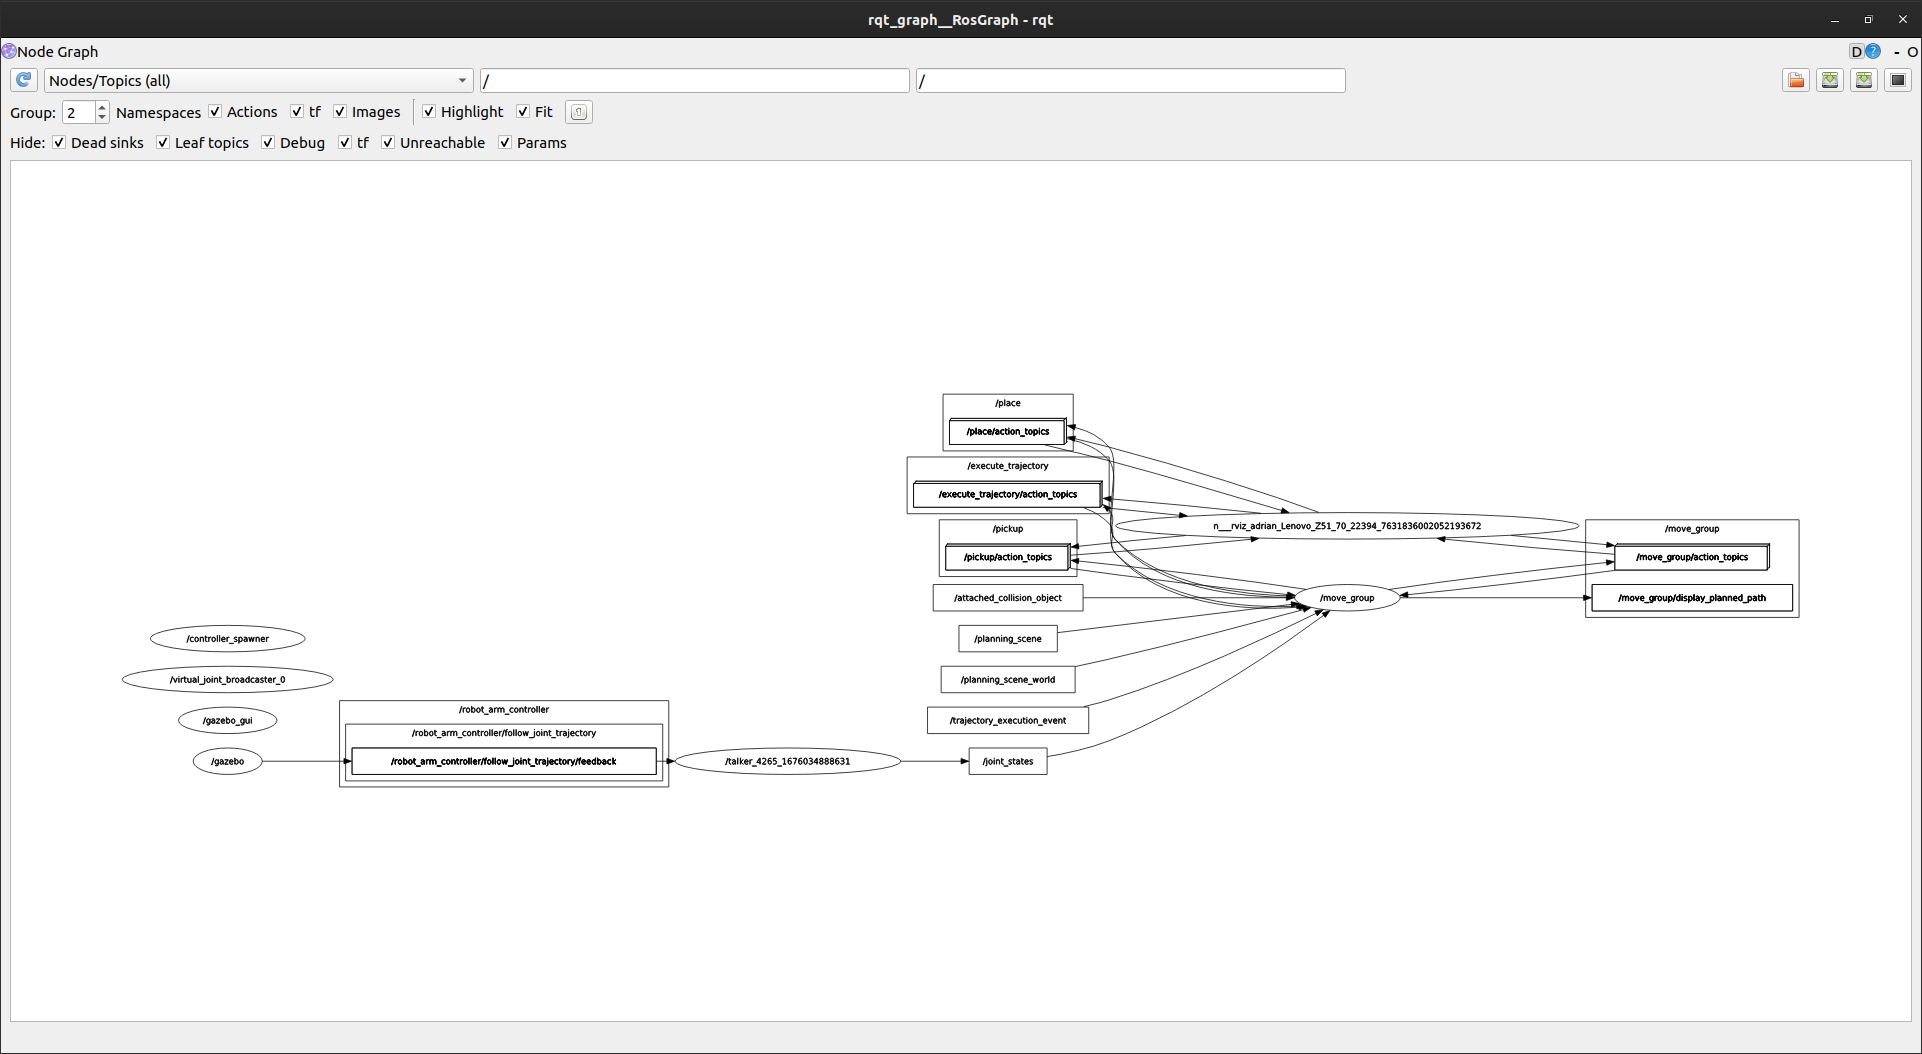
\includegraphics[width=0.9\linewidth]{{img/Bild_rqt.png}}
	\caption{Widok struktury węzłów i tematów ROS w RQR Graphie. \cite{own}}
	\label{fig:7}
\end{figure}

Wyżej wspomniano, iż węzły komunikują się ze sobą w sposób ciągły z wykorzystaniem tematów. Elementy te stanowią swoiste magistrale międzywęzłowe, pozwalające wymieniać wiadomości między nimi. Węzły, które publikują, generują informacje do tematów określane są mianem publisherów (ang. $publisher$), natomiast te które odbierają dane - subskrybentów (ang. $subscriber$). Tematy są zawsze jednokierunkowe, przy czym mogą mieć wielu zarówno publisherów jak i subkrybentów. Jak wspominano tematy służą do komunikacji ciągłej, realizowanej synchronicznie co ustalony kwant czasu, niemniej w przypadku informacji wysyłanych sporadycznie, od czasu do czasu - stosuje się serwisy (ang. $services$).\cite{Topics} 



W systemie rozproszonym, jaki stanowią węzły ROS czasami niezbędne jest wysłanie zapytań i odpowiedzi na nie. Taka jest zatem idea serwisów. Klient wzywa serwis poprzez wysłanie zapytania, a następnie oczekuje odpowiedzi od interesującego go węzła. Przykładowo serwis może dotyczyć wezwania węzła planującego trajektorię do rozpoczęcia tej procedury. \cite{Services}


Ostatnią z głównych składowych oprogramowania ROS są wiadomości (ang. $messages$). To na nich oparta jest komunikacja. W przypadku tematów, wiadomości stanowią struktury danych opakowujące podstawowe typy zmiennych, takie jak integer, double, boolean. Struktury te są często wielopoziomowe, zawierające nierzadko tablice zmiennych.
Natomiast rozpatrując przypadek serwisów, wówczas wiadomości przyjmują postać tak zwanych $request$ $and$ $response$ - zapytań i odpowiedzi, definiowanych w plikach $srv$ ROS. \cite{Msgs}

ROS udostępnia szereg komend, możliwych do uruchomienia z poziomu terminala komputera na którym został zainstalowany. Pozwala wywoływać pliki uruchomieniowe formatu $.launch$. Wtedy to włączane są ustalone zbiory węzłów. Umożliwia to instrukcja $roslaunch$. Możliwe jest jednak uruchomienie tylko jednego wybranego węzła z pomocą komendy $rosrun$. Obie te instrukcje cechuje identyczna składnia. Wpierw należy podać interesującą komendę - $roslaunch$ bądź $rosrun$ natomiast dalej paczkę (ang. $package$), zawierającą docelowy plik i na samym końcu właśnie nazwę pliku wykonawczego, który ma zostać uruchomiony. Istotne jest także by plikowi, który zamierza się uruchomić nadać należyte uprawnienia (instrukcja $chmod$ w Ubuntu), gdyż w przeciwnym wypadku ROS zwraca informację o nie wykrywaniu danego pliku.

Tym samym wspomniano o paczkach ROS. Programy napisane w ROS są pogrupowane w paczki, zawierające węzły, zbiory danych jak również pliki konfiguracyjne (w formcie $.yaml$) jak inne skrypty i pliki wykorzystywane przez dany zbiór. Takie paczki dostarczają konkretną funkcjonalność a jednocześnie są dosyć czytelne dla użytkowników. Ich sporą zaletą jest również duża uniwersalność, gdyż ta sama paczka może współpracować z innymi zbiorami - z czego też korzystano w realizowanym projekcie kontrolera. 

Chcąc stworzyć własny projekt w ROS, użytkownik potrzebuje przygotować opisaną wyżej paczkę. Tak też było w przypadku niniejszego projektu gdzie wygenerowana paczka stanowiła zbiór wszystkich plików zarówno symulujących jak i sterujących posiadanym robotem. 

Paczki można wygenerować automatycznie z pomocą Catkin - dedykowanego kompilatora dołączonego do ROS. Jest to istotne, gdyż każda paczka przed uruchomieniem musi zostać wpierw skompilowana z pomocą Catkina. Na tym etapie do projektu są dołączane także wykorzystywane zależności (ang. $dependencies$), czyli zbiory zewnętrznych bibliotek. Sam proces kompilacji może zająć nierzadko wiele minut, generując przy tym liczne błędy powodujące zatrzymanie się wykonywania procesu. 

\subsection{MoveIt}
MoveIt podobnie jak sam ROS jest otwartoźródłowym projektem przeznaczonym do kontrolowania robotów na poziomie planowania, manipulowania, nawigowania i percepcji trójwymiarowej. MoveIt jest swoistym rozszerzeniem, zbiorem opisywanych w poprzednim podrozdziale paczek, z którego możemy korzystać z poziomu Rviza. Struktura robota jest opisana z pomocą plików URDF. Plik ten uwzględnia geometryczne kształty urządzenia, kinematykę, punkty kolizyjne robota i inne. Dzięki temu po załadowaniu modelu, MoveIt jest w stanie dla ustalonych w pliku URDF grupy złącz robota zaplanować trajektorię ruchu. Tak by osiągnąć docelowy, zadany punkt. Realizuje on zatem zadanie liczenia kinematyki odwrotnej.  \cite{MoveitDoc},  \cite{OMPL_Mov}

\subsection{Rviz}
Rviz stanowi swoisty framework do ROS w postaci graficznego interfejsu użytkownika, w którym to wyświetlanych jest wiele przydatnych dla użytkownika informacji. Rviz pozwala na uruchamianie dodatkowych pluginów - pozwalających np. na ukazanie obrazu z zainstalowanej w robocie kamery bądź zwizualizowanie chmury punktów zwracanej przez lidar. Jak wspomniano Rviz opiera się na pluginach, które po załadowaniu zapewniają określoną przez nie funkcjonalność. Podstawowym pluginem jest $RobotModel$. Zapewnia on wizualizację posiadanego robota. Innym podstawowym pluginem jest $TF$. Zapewnia on wizualizację poszczególnych złącz w jakie zostało wyposażone posiadane urządzenie. Niemniej najistotniejszym pluginem dla rozpatrywanego projektu był właśnie MoveIt. To właśnie w interfejsie Rviz możliwe jest zadawanie pozycji robota, wybór ustawień związanych z planowaniem jak i samo planowanie i rozkazanie jego realizowania.
\cite{Rviz_rep}, \cite{Rviz}


\subsection{Gazebo}


Gazebo stanowi zaawansowane środowisko przeznaczone do symulowania zarówno samego robota jak i otoczenia w którym się znajduje. Pozwala na przetestowanie różnych scenariuszy i strategii poruszania się robota, zanim zostanie on wykorzystany w rzeczywistym projekcie. Wykorzystuje on w swoim działaniu między innymi pliki $URDF$ ($Unified$ $Robotics$ $Description$ $Format$), o których informowano już w poprzednim podroździale poświęconym narzędziu MoveIt. Mogą to być również pliki $XACRO$ bądź $SDF$, które w swojej strukturze są jednak bardzo podobne. 


Gazebo oprócz przestrzeni do symulowania zachowania się robota udostępnia również dwa dodatkowe edytory. Pierwszy z nich umożliwia tworzenie świata, przestrzeni w której użytkownik pragnąłby umieścić swoją maszynę. Natomiast drugi edytor pozwala na zbudowanie wirtualnego modelu urządzenia, a dalej wygenerować go do postaci plików $SDF$ i $config$. Dopiero na dalszym etapie z plików tych z pomocą dodatku MoveIt Setup Asisstant zostanie wygenerowany plik $URDF$. W tym miejscu należy wspomnieć, iż zdarza się, że Gazebo w czasie projektowania modelu robota zawiesza się i ostatecznie cały proces należy rozpocząć od początku. W teorii można zapisywać projekt wraz z kolejnymi etapami budowy modelu robota, niemniej w praktyce po zapisie Gazebo zmienia wszystkie dotychczasowe połączenia ramion. Dodanie kolejnego jest już wówczas bardzo utrudnione.  \cite{Gazebo}
%---------------------------------------------------------------------------

\section{Plannery}
\label{sec:kompilacja}

MoveIt zotał przystosowany do funkcjonowania z wieloma różnymi typami plannerów ścieżek i trajektorii ruchu. W poniższych podrozdziałach pokrótce opisano najważniejsze z nich. 

Pojęcie planowania stanowi kluczowy element robotyki. Jest związane z generowaniem sekwencji sterowań robota w taki sposób by uzyskać zadany ruch bądź przemieszczenie. Istnieje rozróżnienie pomiędzy zagadnieniem planowania ścieżek a planowaniem trajektorii. Czynnikiem rozróżniającym oba pojęcia jest czas. W przypadku trajektorii przemieszczenie robota uwzględnia zależność jego pozycji od konkretnej chwili ruchu. Jest zatem oparte na interpolacji funkcjami wielomianowymi. W przypadku planowania ścieżek istotne są jedynie punkty pierwotne i docelowe, bez uwzględniania pozycji urządzenia pomiędzy nimi. Ścieżki przyjmują kształty geometryczne, mogą również definiować punkty przez które ma przechodzić trasa.

\cite{Gasparetto2015}, \cite{Gasparetto2012}
\cite{MathWorks_planner}

\subsection{OMPL}

OMPL czyli The Open Motion Planning Librarry to swoisty otwartoźródłowy zbiór algorytmów planujących. Zatem biblioteka ta sama w sobie realizuje jedynie kwestie związane ze detekcją kolizji i wizualizacją. Została zaprojekotwana w taki sposób by móc zostać łatwo wykorzystana w innych programach, a jednym z nich jest właśnie wykorzystywany w projekcie MoveIt. Biblioteka OMPL w swoim zbiorze posiada sporo algorytmów planujących takich jak chociażby: PRM, RRT, EST, SBL, KPIECE, SyCLOP. \cite{OMPL}

Pierwszy z wymienionych PRM - $Probabilistic$ $Roadmap$ $Method$ jest plannerem wykorzystującym algorytm oparty na próbkowaniu. W przypadku biblioteki OMPL planner ten został zaimplementowany w oparciu o dwa wątki, gdzie jeden z nich konstruuje ścieżkę (ang. $roadmap$), natomiast drugi sprawdza czy punkty początkowe i końcowe należą do tej ścieżki. OMPL zawiera różne wariancje RPM, różniące się między sobą weryfikacją poszczególnych punktów, wierzchołków roadmapy.

RRT - $Rapidly-exploring$ $Random$ $Trees$ - kolejny dobrze znany planner oparty o algorytm próbkujący. W planerze tym każdy węzeł struktury drzewiastej (ang. $tree$ $ data$ $ structure$) generowany jest w procesie próbkowania losowego. Jak wcześniejszy posiada różne modyfikacje, z których jak najbardziej można korzystać w MoveIt. \cite{8675925}

Natomiast KPIECE - ($Kinematic$ $Planning$ $by$ $Interior-Exterior$ $Cell$ $Exploration$) jest plannerem również opartym o struktury drzewiaste, który wykorzystuje dyskretyzację wielopoziomową do prowadzenia ciągłej eksploracji przestrzeni stanów. 

\cite{MoIt_plan}

\subsection{CHOMP}

Covariant Hamiltonian optimization for motion planning (CHOMP), czyli jak wskazuje angielska definicja jest to procedura służaca planowaniu trajektorii poruszania się łańcucha kinematyczego oparta o optymalizację gradientową. Algorytm ten wykorzystuje podejście gradientowe w celu ustalenia optymalnej trajektorii. \cite{CHOMP}

\subsection{Pilz Industrial Motion Planner}

Planner ten pozwala na generowanie podstawowych trajektorii robota takich jak PTP (ang. $Point-to-Point$), LIN (ang. $Linear$) oraz CIRC (ang. $Circular$). Planner ten cechuje prostota. W zastosowaniach przemysłowych czasami konieczne jest zwykłe przemieszczenie robota w linii prostej. Takie też, bez zbędnych udziwnień dostarcza tenże planner. Nazwa algorytmu tego pochodzi od niemieckiej firmy, która jest odpowiedzialna za stworzenie tego plannera. Poprzez swą prostotę algorytm ten nie potrafi omijać przeszkód. Fakt ten został również zaobserwowany w czasie późniejszych testów. Planner ten jest jedynie generatorem ruchu, przez co właśnie po wyznaczeniu trajektorii, algorytm sprawdza czy nie występuje nigdzie kolizja. Jeżeli takowa występuje, wówczas zwraca informację o nieudanej próbie wyznaczenia trajektorii.  \cite{Pilz_AG}

%---------------------------------------------------------------------------

\section{Mikrokontrolery}
\label{sec:narzedzia}

Mikrokontrolery, których w projekcie sumarycznie wykorzystano aż cztery, są układami cyfrowymi zawartymi w jednym układzie scalonym, składającymi się z mikroprocesora i dedykowanych peryferiów. Całość pozwala na autonomiczną pracę, czyli w skrajnym przypadku do jego funkcjonowania nie jest wymagany żaden dodatkowy układ pomocniczy. Mikrokontrolery są przystosowane do pracy jako elementy sterujące bądź kontrolno-pomiarowe.

Poniżej przytoczono kilka najważniejszych informacji na temat dwóch układów o jakie rozbudowano robota na potrzeby implementacji kontrolera ROS. \cite{MiM_wyk} 

\subsection{ESP8266}

ESP8266 stanowi wysoce zintegrowany mikrokontroler wyposażony w moduł Wi-Fi, z przeznaczeniem głównie do wykorzystania w urządzeniach internetu rzeczy (ang. $Interenet$ $of$ $Things$). Głównymi zaletami są również kompaktowa budowa, niskie zużycie energii oraz wysoką efektywność.\cite{ESP_doc}


Mikrokontroler ESP8266 na potrzeby projektu programowano w języku C. Wykorzystywano w tym celu $toolchain$ do budowania aplikacji oraz $ESP8266\_RTOS\_SDK$ czyli oprogramowanie udostępniające API do ESP, a także skrypty pozwalające obsługiwać $toolchain$. Zatem sam mikrokontroler działał w oparciu o pseudosystem operacyjny FreeRTOS. Pozwalało to na napisanie w prosty sposób aplikacji wielowątkowej, co okazało się bardzo przydatne dla realizowanego zadania odczytu enkoderów. \cite{ESP_prog}

%W poniższej tabeli zamieszczono najważniejsze parametry mikrokontrolera ESP8266.


W przypadku omawianego mikrokontrolera należy również wspomnieć o konieczności dodawania do przynajmniej jednego wątku instrukcji kasującej licznik $watchdoga$. Zatem nie jest to realizowane domyślnie przez FreeRTOS, spoczywa to na barkach osoby piszącej program. Bez komendy tej urządzenie będzie się regularnie resetowało. 

Natomiast drugą kwestią jest wykorzystanie niektórych pinów GPIO. W momencie restartu mikrokontrolera, pewne wybrane piny nie mogą posiadać określonych stanów logicznych - wysokich bądź niskich, gdyż to powoduje zmianę trybu bootowania urządzenia, a przez procesor może nie chcieć się uruchomić. O ile funkcjonalność ta w pewnych przypadkach może być jak najbardziej porządna, niemniej należy mieć na uwadze takie, a nie inne zachowanie się ESP8266.

Należy również podkreślić, iż wykorzystywany w projekcie mikrokontroler ESP był w postaci płytki rozwojowej NodeMCU w wersji V3. Najważniejsze jej specyfikacje umieszczono poniżej - tabela \ref{tab:1}.

% Please add the following required packages to your document preamble:
% \usepackage[table,xcdraw]{xcolor}
% If you use beamer only pass "xcolor=table" option, i.e. \documentclass[xcolor=table]{beamer}
\begin{table}[H]
\centering
\caption{Najważniejsza specyfikacja płytki rozwojowej NodeMCU V3 \cite{ESP_param}}
\label{tab:1}
\begin{tabular}{|c|c|c|c|ll}
\cline{1-4}
\cellcolor[HTML]{C0C0C0}L.p. & \cellcolor[HTML]{C0C0C0}Parametr          & \cellcolor[HTML]{C0C0C0}Opis, wartość                          & \cellcolor[HTML]{C0C0C0}Jednostka &  &  \\ \cline{1-4}
\cellcolor[HTML]{EFEFEF}1.   & \cellcolor[HTML]{EFEFEF}Mikrokontroler    & \cellcolor[HTML]{EFEFEF}Tensilica 32-bit RISC CPU Xtensa LX106 & \cellcolor[HTML]{EFEFEF}-         &  &  \\ \cline{1-4}
\cellcolor[HTML]{C0C0C0}2.   & \cellcolor[HTML]{C0C0C0}Taktowanie zegara & \cellcolor[HTML]{C0C0C0}80                                     & \cellcolor[HTML]{C0C0C0}MHz       &  &  \\ \cline{1-4}
\cellcolor[HTML]{EFEFEF}3.   & \cellcolor[HTML]{EFEFEF}Napięcie pracy    & \cellcolor[HTML]{EFEFEF}3.3                                    & \cellcolor[HTML]{EFEFEF}V         &  &  \\ \cline{1-4}
\cellcolor[HTML]{C0C0C0}4.   & \cellcolor[HTML]{C0C0C0}Pamięć Flash      & \cellcolor[HTML]{C0C0C0}4                                      & \cellcolor[HTML]{C0C0C0}MB        &  &  \\ \cline{1-4}
\cellcolor[HTML]{EFEFEF}5.   & \cellcolor[HTML]{EFEFEF}Pamięć SRAM       & \cellcolor[HTML]{EFEFEF}128                                    & \cellcolor[HTML]{EFEFEF}KB        &  &  \\ \cline{1-4}
\cellcolor[HTML]{C0C0C0}6.   & \cellcolor[HTML]{C0C0C0}Ilość pinów GPIO  & \cellcolor[HTML]{C0C0C0}17                                     & \cellcolor[HTML]{C0C0C0}-         &  &  \\ \cline{1-4}
\cellcolor[HTML]{EFEFEF}7.   & \cellcolor[HTML]{EFEFEF}Wbudowane WiFi    & \cellcolor[HTML]{EFEFEF}802.11 b/g/n                           & \cellcolor[HTML]{EFEFEF}-         &  &  \\ \cline{1-4}
\cellcolor[HTML]{C0C0C0}8.   & \cellcolor[HTML]{C0C0C0}Magistrale        & \cellcolor[HTML]{C0C0C0}UART/I2C/SPI                           & \cellcolor[HTML]{C0C0C0}-         &  &  \\ \cline{1-4}
\cellcolor[HTML]{EFEFEF}9.   & \cellcolor[HTML]{EFEFEF}Przetworniki      & \cellcolor[HTML]{EFEFEF}Jeden ADC                              & \cellcolor[HTML]{EFEFEF}-         &  &  \\ \cline{1-4}
\end{tabular}
\end{table}

\subsection{Raspberry Pi4B}

Raspberry Pi 4B stanowił w momencie pisania niniejszej pracy najnowsze wydanie popularnej serii mikrokomputerów brytyjskiej organizacji Raspberry Pi Foundation. Urządzenie to oprócz dostarczania podstawowej funkcjonalności spotykanej w komputerach klasy PC, udostępnia użytkownikowi również 28 pinów GPIO (ang. $General$ $Purpose$ $Input$ $Output$) - podobnie jak klasyczny mikrokontroler. Najważniejsze parametry mikrokomputera RPI4B wymieniono w poniższej tabeli \ref{tab:2}.


\begin{table}[H]
\centering
\caption{Najważniejsza specyfikacja mikrokomputera Raspberry Pi4B \cite{RPI_par}}
\label{tab:2}
\begin{tabular}{|c|c|c|c|ll}
\cline{1-4}
\cellcolor[HTML]{C0C0C0}L.p. & \cellcolor[HTML]{C0C0C0}Parametr          & \cellcolor[HTML]{C0C0C0}Opis, wartość                   & \cellcolor[HTML]{C0C0C0}Jednostka &  &  \\ \cline{1-4}
\cellcolor[HTML]{EFEFEF}1.   & \cellcolor[HTML]{EFEFEF}Procesor          & \cellcolor[HTML]{EFEFEF}Quad core 64-bit ARM-Cortex A72 & \cellcolor[HTML]{EFEFEF}-         &  &  \\ \cline{1-4}
\cellcolor[HTML]{C0C0C0}2.   & \cellcolor[HTML]{C0C0C0}Taktowanie zegara & \cellcolor[HTML]{C0C0C0}1.5                             & \cellcolor[HTML]{C0C0C0}GHz       &  &  \\ \cline{1-4}
\cellcolor[HTML]{EFEFEF}3.   & \cellcolor[HTML]{EFEFEF}Pamięć RAM        & \cellcolor[HTML]{EFEFEF}2, 4, 8 (w projekcie użyto 8)   & \cellcolor[HTML]{EFEFEF}GB        &  &  \\ \cline{1-4}
\cellcolor[HTML]{C0C0C0}4.   & \cellcolor[HTML]{C0C0C0}Bluetooth         & \cellcolor[HTML]{C0C0C0}5.0 z Bluetooth Low Energy      & \cellcolor[HTML]{C0C0C0}-         &  &  \\ \cline{1-4}
\cellcolor[HTML]{EFEFEF}5.   & \cellcolor[HTML]{EFEFEF}Wbudowane WiFi    & \cellcolor[HTML]{EFEFEF}802.11 b/g/n/ac                 & \cellcolor[HTML]{EFEFEF}-         &  &  \\ \cline{1-4}
\cellcolor[HTML]{C0C0C0}6.   & \cellcolor[HTML]{C0C0C0}Ilość pinów GPIO  & \cellcolor[HTML]{C0C0C0}28 (w tym PWM i GPCLK)          & \cellcolor[HTML]{C0C0C0}sztuk     &  &  \\ \cline{1-4}
\cellcolor[HTML]{EFEFEF}7.   & \cellcolor[HTML]{EFEFEF}Porty USB         & \cellcolor[HTML]{EFEFEF}2 x 2.0 i 2 x 3.0               & \cellcolor[HTML]{EFEFEF}sztuki    &  &  \\ \cline{1-4}
\cellcolor[HTML]{C0C0C0}8.   & \cellcolor[HTML]{C0C0C0}Magistrale        & \cellcolor[HTML]{C0C0C0}UART/I2C/SPI/SDIO/DPI/PCM       & \cellcolor[HTML]{C0C0C0}-         &  &  \\ \cline{1-4}
\cellcolor[HTML]{EFEFEF}9.   & \cellcolor[HTML]{EFEFEF}Porty micro-HDMI  & \cellcolor[HTML]{EFEFEF}2                               & \cellcolor[HTML]{EFEFEF}sztuki    &  &  \\ \cline{1-4}
\cellcolor[HTML]{C0C0C0}10.  & \cellcolor[HTML]{C0C0C0}Port SD Card      & \cellcolor[HTML]{C0C0C0}1                               & \cellcolor[HTML]{C0C0C0}sztuka    &  &  \\ \cline{1-4}
\end{tabular}
\end{table}

 Wszystkie te parametry sprawiają, iż układ w pewnym stopniu może nawet zastąpić komputer osobisty. O ile użytkowanie go jako urządzenie multimedialne, mimo iż jest to możliwe, to jest to raczej mało praktyczne, o tyle wykorzystanie w projektach podobnych do opisywanego w niniejszej pracy jest jak najbardziej wskazane. W takich sytuacja oferowana moc obliczeniowa jest wystarczająca.

Jako iż Raspberry posiada w swojej budowie piny GPIO, toteż teoretycznie, sam ten mikrokomputer mógłby być wykorzystywany do obsługi zarówno enkoderów, czujników jak i do sterowania silnikami krokowymi robota. Zatem dwa dodatkowe mikrokontrolery STM oraz ESP mogą wydawać się naddatkowe. Niemniej realizując projekt zamierzano rozszerzyć obecną funkcjonalność a nie ją zastępować. Toteż nie chciano porzucać już wypracowanych rozwiązań. Natomiast drugą kwestią, możliwe że nawet istotniejszą jest kwestia zabezpieczenia mikrokomputera Raspberry Pi przed uszkodzeniem. W czasie realizacji projektu inżynierskiego, w czasie prób, uszkodzono pierwotny mikrokontroler STM32 (doprowadzając przez przypadek do zwarcia), toteż chcąc nie dopuścić do podobnej sytuacji w przypadku RPI4B postanowiono nie instalować go w miejsce STM32, tylko połączyć z nim poprzez przewód USB.


%---------------------------------------------------------------------------

\section{Podsumowanie rozdziału}

Podsumowując niniejszy rozdział, można napisać, iż co prawda projekt łączy w sobie wiele różnych zagadnień, niemniej starano się je w sposób zwięzły i zrozumiały przytoczyć. Wiele kwestii zostało znacznie spłyconych i przez to okrojonych, niemniej np. tematyka plannerów jest tak złożona, iż prawdopodobnie zagłębianie się w szczegóły mogłoby mijać się z celem. Są to tematy poruszane przez wiele artykułów naukowych, planowanie optymalnej ścieżki, w możliwie najkrótszym czasie, z uwzględnieniem towarzyszących robotowi przeszkód stanowi problem badawczy, którym zajmują się naukowcy z całego świata. Celem projektu było między innymi porównanie tychże plannerów w swoim działaniu pomiędzy sobą, natomiast mniej analizowanie dokładnie mechaniki na której się opierają.

W rozdziale tym starano się też wspominać o pewnych kwestiach, które okazują się przydatne przy bezpośredniej implementacji zadań, tak jak to miało chociażby miejsce w przypadku ESP8266 - wspominając o jego zachowaniu przy restarcie. Wiedza taka może zaoszczędzić sporo czasu.

\label{sec:przygotowanieDokumentu}


	\chapter{Realizacja projektu}

Praktyczną realizację projektu podzielono na dwie części. Pierwsza z nich dotyczyła zmian sprzętowych, koniecznych do zaimplementowania w robocie, natomiast druga część związana była z pracami programistycznymi jakie należało przeprowadzić. Poniżej dokładnie opisano cały proces.

\section{Prace sprzętowe}

W niniejszej sekcji przybliżono prace sprzętowe jakie wykonano nad robotem by móc go przystosować do tworzonego kontrolera. Manipulator, którym dysponowano po projekcie inżynierskim rozbudowano o dodatkowe mikrokontrolery oraz enkodery, tak by móc zaimplementować na nim docelowy kontroler ROS. 

\subsection{Montaż enkoderów}
Pierwszą kwestią jaką się zajęto związana była z zainstalowaniem enkoderów każdej osi.

Silniki krokowe wykorzystywane w robocie, w czasie swojej pracy wykonują jednostkowe kroki, przez co teoretycznie możliwe jest na tej podstawie stwierdzanie w jakim położeniu znajduje się dana oś robota. Można po prostu liczyć wykonane kroki. Teoretycznie takie rozwiązanie mogłoby być wystarczające w zbudowanym robocie, niemniej w zastosowaniach praktycznych raczej zawsze wykorzystuje się dodatkowe czujniki - enkodery. Pozwala to na mierzenie faktycznych ruchów poszczególnych osi. Oczywistym jest przecież, iż oś może być zablokowana bądź silnik po prostu zgubi kroki i przez to nie wykona żądanego odchylenia danego złącza. Tym samym informując kontroler o wykonaniu kroków, których tak naprawdę robot nie podjął, prowadzi to do sytuacji, kiedy to sterownik wykona planowanie w oparciu o błędne wskazania, a to przełoży się na dalsze przekłamania. Dysponując enkoderami kontroler będzie w stanie zgłosić błąd, jeśli ruch osi się nie odbył.


Zatem by sterownik robota mógł operować na faktycznych pomiarach przemieszczeń poszczególnych osi, postanowiono doposażyć robota w enkodery. Ze względu na różną specyfikę każdych złącz, w zależności od możliwości, montowano inne czujniki. Tak więc na części osi robota zamontowano enkodery REM5, natomiast na pozostałych posłużono się czujnikami szczelinowymi wraz z odpowiednio zamodelowanymi tarczami przysłonowymi. Pierwsze rozwiązanie jest znacznie dokładniejsze aniżeli to drugie, niemniej w żadnym przypadku rozdzielczość enkoderów nie jest mniejsza niż luz występujący na danym złączu (pomijając ramię główne, gdzie luz nie występuje). Jak wiadomo robot powstał w oparciu o metodę wydruku 3D, przez co przejawia pewne niedoskonałości, objawiające się chociażby wspomnianym luzem. 

O ile co do stosowania impulsatorów REM5 w odniesieniu do osi ramienia głównego, ramienia drugiego oraz trzeciego, nie było większych wątpliwości i trudności ich implementacji, o tyle długo zastosowano się nad obrotową wieżą. Ze względu na brak miejsca, nie było możliwości zamontowania enkodera na wale silnika, toteż zaproponowano poniższe rozwiązanie - rysunek \ref{fig:5}.

 \begin{figure}[H]
	\centering
	\includegraphics[width=0.9\linewidth]{{img/Bild_enkoder.jpg}}
	\caption{\centering Widok stworzonego enkodera obrotowej wieży oraz ramienia trzeciego. \cite{own}}
	\label{fig:5}
\end{figure}



Jak można zauważyć, do zliczania kątów odchyleń wieży, posłużono się dwoma czujnikami optycznymi umieszczonymi w specjalnie tym celu zamodelowanym mocowaniu. Przez szczeliny wspomnianych czujników przebiega swoista drabinka. Jest ona na stałe przymocowana do obrotowej wieży, natomiast czujniki optyczne do podstawy. Przez fakt, iż z punktu widzenia szczebli drabinki, czujniki są przesunięte względem siebie geometrycznie o kąt 90 stopni, sygnały jakie zwracają wraz z obracaniem wieży, to dwie przesunięte fale prostokątne. Uzyskano zatem klasyczny enkoder. W ten sposób możliwe jest zarówno zliczanie kątów jak i wyznaczanie kierunku ruchu.
Rozwiązanie to, mimo iż jego rozdzielczość jest mniejsza niż w przypadku pozostałych osi, to nadal jest bardziej precyzyjne, niż obecny na złączu naturalny luz.

Na rysunku \ref{fig:5} możliwe jest do zaobserwowania także mocowanie impulsatora REM5 do jednego z silników napędowych. We wszystkich pozostałych osiach, w których stosowano te enkodery wyglądało to podobnie, toteż już tego nie ilustrowano. Jako, iż enkodery te posiadają rozdzielczość 80 impulsów na obrót, to po uwzględnieniu przekładni napędzających je, otrzymywana dokładność jest znaczna. Dokładne zestawienie liczbowe zaprezentowano w  tabeli \ref{tab:3}.

Problematyczna okazała się także ostatnia z osi robota - obrót chwytaka. W tej sytuacji również nie było miejsca na zamontowanie enkodera REM5. Stwierdzono, iż ze względu na zastosowanie przekładni ślimakowej do jej napędzania - jej ruch możliwy jest jedynie włączając silnik napędowy. Z tego powodu zaproponowano poniższe rozwiązanie - rysunek \ref{fig:55}. 

 \begin{figure}[H]
	\centering
	\includegraphics[width=0.9\linewidth]{{img/Bild_enkoder_chwytak.jpg}}
	\caption{Widok enkodera osi obracającej chwytak. \cite{own}}
	\label{fig:55}
\end{figure}

Zainstalowany czujnik szczelinowy wraz z obrotem wału silnika wykrywa ruch tarczy przesłonowej, w wyniku czego możliwe jest liczenie impulsów przez mikrokontroler ESP8266. Natomiast kierunek ruchu ustalany jest na podstawie kierunku obrotu silnika. Jak wspominano nie ma innej możliwości poruszenia tąże osią, jak tylko włączając silnik. Samohamowność przekładni ślimakowej oraz miejsce umieszczenia wału silnika wewnątrz ramienia drugiego, niwelują możliwy wpływ czynników grawitacji i ingerencji użytkownika w ruch złącza.

Należy również nadmienić, iż podobnie jak to miało miejsce w przypadku projektowania całego manipulatora, tak i obecnie, w odniesieniu do wszelkich mocowań enkoderów, tarcz i drabinek przesłonowych - modelowanie tych elementów realizowano w programie Autodesk Inventor Professional 2021. Modele po wyeksportowaniu do formatu plików $.stl$ zamieniano na ciąg $.gcode$ w oprogramowaniu KISSlicer, a ostatecznie drukowano na drukarce Prusa i3 wyposażonej w otwartoźródłowe oprogramowanie Marlin. Stosowano filament PLA.

Poniżej w jednej tabeli zestawiono parametry wszystkich zainstalowanych enkoderów - tabela \ref{tab:3}

% Please add the following required packages to your document preamble:
% \usepackage[table,xcdraw]{xcolor}
% If you use beamer only pass "xcolor=table" option, i.e. \documentclass[xcolor=table]{beamer}
\begin{table}[H]
\caption{Zestawienie rozdzielczości poszczególnych enkoderów}
\label{tab:3}
\begin{tabular}{|c|c|c|
>{\columncolor[HTML]{C0C0C0}}c |c|
>{\columncolor[HTML]{C0C0C0}}c |ll}
\cline{1-6}
\cellcolor[HTML]{C0C0C0}L.p. & \cellcolor[HTML]{C0C0C0}Złącze         & \cellcolor[HTML]{C0C0C0}\begin{tabular}[c]{@{}c@{}}Rozdzielczość \\ enkodera {[}imp./obrót{]}\end{tabular} & \begin{tabular}[c]{@{}c@{}}Przekładnia\\ złącza\end{tabular} & \cellcolor[HTML]{C0C0C0}\begin{tabular}[c]{@{}c@{}}Rozdzielczość kątowa\\  złącza {[}°/obrót{]}\end{tabular} & \begin{tabular}[c]{@{}c@{}}Luz \\ złącza {[}st{]}\end{tabular} &  &  \\ \cline{1-6}
\cellcolor[HTML]{EFEFEF}1.   & \cellcolor[HTML]{EFEFEF}Obrót wieży    & \cellcolor[HTML]{EFEFEF}256                                                                                & \cellcolor[HTML]{EFEFEF}1                                    & \cellcolor[HTML]{EFEFEF}1° 24'                                                                               & \cellcolor[HTML]{EFEFEF}2° 50’                                 &  &  \\ \cline{1-6}
\cellcolor[HTML]{C0C0C0}2.   & \cellcolor[HTML]{C0C0C0}Ramię główne   & \cellcolor[HTML]{C0C0C0}80                                                                                 & 72                                                           & \cellcolor[HTML]{C0C0C0}0° 3' 45''                                                                           & Brak                                                           &  &  \\ \cline{1-6}
\cellcolor[HTML]{EFEFEF}3.   & \cellcolor[HTML]{EFEFEF}Ramię drugie   & \cellcolor[HTML]{EFEFEF}80                                                                                 & \cellcolor[HTML]{EFEFEF}14.0625                              & \cellcolor[HTML]{EFEFEF}0° 19' 12''                                                                          & \cellcolor[HTML]{EFEFEF}3° 05’                                 &  &  \\ \cline{1-6}
\cellcolor[HTML]{C0C0C0}4.   & \cellcolor[HTML]{C0C0C0}Ramię trzecie  & \cellcolor[HTML]{C0C0C0}80                                                                                 & 15                                                           & \cellcolor[HTML]{C0C0C0}0° 18' 0''                                                                           & 2° 41’                                                         &  &  \\ \cline{1-6}
\cellcolor[HTML]{EFEFEF}5.   & \cellcolor[HTML]{EFEFEF}Obrót chwytaka & \cellcolor[HTML]{EFEFEF}36                                                                                 & \cellcolor[HTML]{EFEFEF}25                                   & \cellcolor[HTML]{EFEFEF}0°  24' 0''                                                                          & \cellcolor[HTML]{EFEFEF}4° 3’                                  &  &  \\ \cline{1-6}
\end{tabular}
\end{table}

\subsection{Implementacja mikrokontrolera Raspberry Pi i ESP}

Enkodery należało oczywiście należycie podłączyć do mikrokontrolera, z którym współpracowały. W tym celu wykorzystano cienkie przewody pochodzące od przewodu Ethernetowego. Zasadniczo wszystkie czujniki robota łączono w ten sposób. Na końcach dolutowywano jeszcze wymagane zakończenia typu $goldpin$ - w zależności od potrzeb męskie bądź żeńskie.

Natomiast mikrokontroler STM32 był podłączony do sterowników silników krokowych jeszcze w ramach projektu inżynierskiego. Podobnie czujniki do bazowania, toteż nie było konieczności ingerencji w te elementy. Wystarczyło zatem sprząc STM32 z mikrokomputerem RPi4B z pomocą przewodu USB. 

Poniżej widok robota z profilu, przysposobionego w enkodery - rysunek \ref{fig:8}

 \begin{figure}[H]
	\centering
	\includegraphics[width=0.9\linewidth]{{img/Bild_unface.jpg}}
	\caption{\centering Widok robota z profilu. \cite{own}}
	\label{fig:8}
\end{figure}

Jak już możliwe jest do zaobserwowania - ilość przewodów biegnąca do roota jest znaczna. Jest to jeden z problemów jaki należałoby ewentualnie w przyszłości rozwiązać, gdyż przewody te stanowią utrudnienie w poruszaniu się manipulatora. Szczególnie niekorzystnie wpływają na możliwość jego obracania.

\section{Prace programistyczne}




\subsection{Oprogramowanie ESP - odczyt enkoderów}

Enkodery sprzężono z mikrokontrolerem ESP8266. Urządzenie to zaprogramowano napisanym kodem w języku C. Program wykorzystuje pseudosystem operacyjny FreeRTOS, na którym uruchomionych jest pięć osobnych wątków. Każdy wątek odpowiada za obsługę osobnego enkodera.

Pisanie oprogramowania na mikrokontroler ESP z wykorzystaniem $ESP8266\_RTOS\_SDK$ cechuje pewien narzucony schemat. Zatem w pierwszej kolejności niezbędne było określenie funkcji poszczególnych pinów. Wybrano toteż 9 możliwych do wykorzystania portów GPIO i określono ich funkcję jako piny wejściowe. Niestety 2 z używanych pinów pełnią istotną rolę przy starcie mikrokontrolera, przez co nie mogą przyjmować określonych stanów. Uwzględniając ten fakt, koniecznym jest odłączanie ich w momencie podłączania ESP do zasilania (podłączania przewodu USB do Raspberry Pi). 
W dalszej kolejności program inicjalizował wątki. Całość nie wykorzystuje systemu przerwań, jednak cyklicznie odczytuje stan każdego z podłączonych pinów. Każdy odczyt działa z okresem 10 milisekund.

Niestety enkodery nie są urządzeniami idealnymi. W związku z tym moment ich przełączania wiąże się z generacją swoistych drgań. Przejściu z jednego stanu do drugiego towarzyszą wielokrotne przełączenia wartości między tymi dwoma stanami. Jest to tak zwany $bouncing$. By program błędnie nie naliczał dodatkowych kroków wywołanych powyższym zjawiskiem zaimplementowano w programie prostą maszynę stanów zrealizowaną na instrukcji $switch$ języka C. Rozwiązanie to zupełnie rozwiązuje opisany problem. \cite{ESP_enc_file} 

Ostatnią kwestią było wysyłanie pomiarów przez port USB do mikrokomputera Raspberry Pi. Pierwotnie zakładano wysyłanie danych każdorazowo, po odnotowanej zmianie stanu danego enkodera. Niemniej później zrezygnowano z tego pomysłu, na rzecz stałej, synchronicznej wysyłki co 0.1 sekundy, bez względu na wystąpienie ruchu osi czy też nie. 

Poniżej widok  mikrokontrolera ESP8266 wraz z podpiętymi przewodami enkoderów - rysunek \ref{fig:6}. Poszczególne przewody zostały podpisane co ułatwiało późniejsze rozróżnienie ich.

 \begin{figure}[H]
	\centering
	\includegraphics[width=0.8\linewidth]{{img/Bild_ESP.jpg}}
	\caption{\centering Mikrokontroler ESP8266 wraz z podpiętymi przewodami enkoderów. \cite{ESP_enc_file}, \cite{own}}
	\label{fig:6}
\end{figure}

\subsection{Oprogramowanie Raspberry Pi}

Stworzony kontroler robota, tak jak to ukazano na poniższym rysunku \ref{fig:4}, zrealizowano w taki sposób, iż wszystkie najważniejsze obliczenia związane z planowaniem trasy realizowane są na laptopie, na którym też uruchomiony jest rdzeń ROSa (laptop pełni rolę mastera). Natomiast na mikrokontrolerze Raspberry Pi uruchamiano dwa węzły (node'y) ROSa. Jeden związany był z subskrybowaniem sygnałów sterujących pochodzących od plannera trajektorii. Węzeł ten wysyłał przeliczone ruchy poszczególnych złącz na ilości kroków do wykonania do mikrokontrolera STM, który to już sterował silnikami. Natomiast drugi węzeł - publisher wysyłał aktualne pozycje poszczególnych złącz z enkoderów. Informacje te otrzymywał z podłączonego poprzez port USB mikrokontrolera ESP8266. Subkryber i publisher uruchomione są jako dwa osobne wątki w programie napisanym w języku Python. Przy czym wątki te komunikują się ze sobą. \cite{Rasp_node_file}

%Realizując projekt zaproponowano niniejszą koncepcję połączenia poszczególnych elementów ze sobą - rysunek \ref{fig:4}

 \begin{figure}[H]
	\centering
	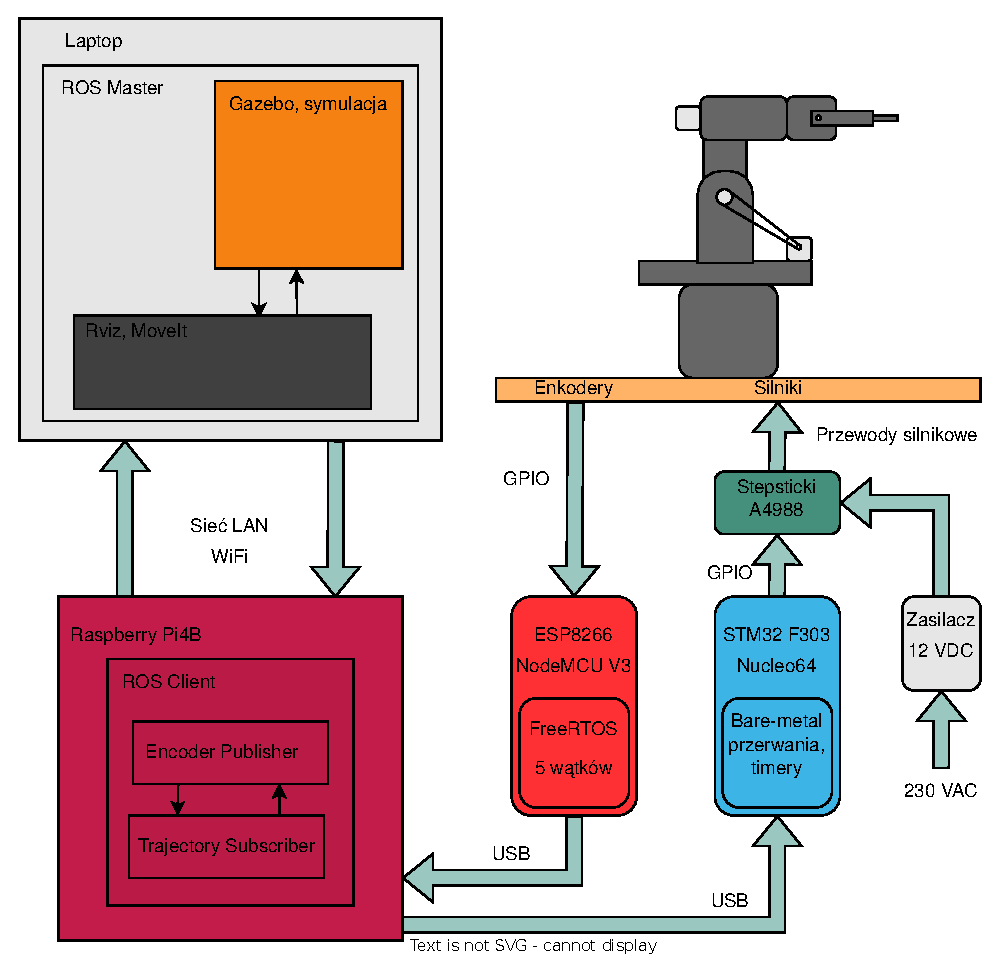
\includegraphics[width=0.9\linewidth]{{img/Bild_schemat.eps}}
	\caption{\centering Schemat połączeń poszczególnych elementów ze sobą. \cite{own}}
	\label{fig:4}
\end{figure}

Węzeł publikujący zrealizowano w taki sposób, iż w nieskończonej pętli "nasłuchuje" on wiadomości nadchodzących z ESP. Informacje te składają się z litery oraz liczby. Pierwsza litera informuje Raspberry Pi jakiego złącza dotyczy otrzymana wiadomość, natomiast liczba - o pozycji osi odczytanej z enkoderów. Węzeł ten synchronicznie publikuje wiadomości. Czyni to z częstotliwością 10 Hz do tematu $/joint\_state$.

Natomiast węzeł subskrybujący nasłuchuje wiadomości otrzymywanych od Mastera ROS (od laptopa). Dotyczy on tematu $/execute\_trajectory/goal$. Zatem w momencie otrzymania wiadomości wyciąga on z niej pozycje wszystkich złącz oraz ich prędkości. Następnie tłumaczy je na konkretne ilości kroków poszczególnych silników. Podobnie uwzględnia ich prędkość oraz kierunek ruchu. Ostatecznie formuje 32 znakową wiadomość, którą wysyła portem szeregowym do mikrokontrolera STM32. W niej zapisane są kierunki, prędkości oraz kroki do wykonania każdej osi. 

Przy czym istotne jest także, iż opisywany subskrybent rozróżnia sterowania dotyczące ramienia robota oraz samego chwytaka. Jeżeli kontroler ROS wysłał informację o ruchu chwytaka, wówczas wszystkie pola 32 znakowej ramki są zerami, z wyjątkiem dwóch ostatnich, gdzie subskrybent koduje informacje o nowej pozycji członu chwytającego.

iż w zależności czy sterowanie dotyczy ramienia robota czy samego chwytaka to subskrybent ten jest w stanie

Pisanie węzłów ROSa w języku Python dawało pewne ułatwienie aniżeli wykorzystując w tym celu język C++. Python nie wymaga kompilacji, jest językiem interpretowanym. W związku z tym napisany kod mógł być od razu uruchomiony instrukcją $rosrun$. Wszelkie publishery oraz subscribery napisane w C++ wymagałyby instrukcji $catkin$ $build$. Z kolei proces budowania, w momencie gdy aplikacja wykorzystywała liczne dodatkowe paczki ROSa, może być bardzo problematyczny do przeprowadzenia. Nierzadko pojawiają się liczne błędy związane z linkowaniem bibliotek, o których częściowo napisano w rozdziale 3.2.4. Dodatkowo gdy proces odbywa się na mikrokomputerze Raspberry Pi problemy te jedynie się nasilają.

Istotną kwestią, która zajęła sporo czasu był sam wybór systemu operacyjnego dla mikrokomputera Raspberry Pi. Sumarycznie przetestowano około 5 różnych systemów i dopiero ostatni spełniał wszystkie pożądane cechy - możliwe było na nim zainstalowanie ROSa Noetic oraz posiadał interfejs graficzny. Systemem tym okazał się Ubuntu Mate 20.04 przeznaczonym pod procesory ARM. Klasyczny Raspberry Pi OS nie posiadał w swoim repozytorium ROSa do zainstalowania, Ubuntu 22.04 pozwalało na zainstalowanie ROS, natomiast nie w dystrybucji Noetic, Ubuntu Server 20.04 pozwalał na zainstalowanie ROS Noetic, niemniej ze względu na brak interfejsu graficznego postanowiono go porzucić. Najprostsze podłączenie do sieci WiFi wiązało się wówczas z mozolnym wpisywaniem instrukcji do terminala. Pisanie jakiegokolwiek kodu w notatniku typu VIM nie jest optymalnym rozwiązaniem.


Jako iż robot posiada konstrukcję, w której silniki napędowe umieszczono w większości przy podstawie, toteż warunkuje to sposób zachowania się poszczególnych złącz urządzenia. Przede wszystkim poruszając ramieniem drugim manipulatora, porusza się jednocześnie obrotowa końcówka robota. Toteż chcąc utrzymać ją w niezmienionej pozycji, niezbędne jest kompensowanie ruchu ramienia drugiego, sterując również złączem ramienia trzeciego. Kompensację tę zrealizowano w sposób programowy i dlatego też oba węzły uruchamiane na mikrokomputerze Raspberry Pi komunikują się - tak by możliwe było kompensowanie wskazań enkoderów o ruchy związane z korektą pozycji niezbędną do utrzymania ramion zależnych od siebie w niezmienionej pozycji. Okazuje się iż znając między innymi przekładnie poszczególnych napędów osi można w precyzyjny sposób wyznaczyć tę kompensację.

Komunikacja między masterem uruchomionym na laptopie a ROSem pracującym na Rapberry Pi odbywała się przez Internet. Przy czym oba urządzenia musiały znajdować się w tej samej sieci lokalnej. W innym wypadku niezbędny musiałby być VPN, jednak rozwiązania tego nie testowano, gdyż nie było nawet takiej potrzeby. Niemniej możliwość taka istniała.

By komunikacja między urządzeniami zachodziła poprawnie niezbędne okazało się uruchomienie między nimi synchronizacji czasu, gdyż w przeciwnym wypadku ROS zgłaszał uwagi, iż pozycje poszczególnych złącz jakie otrzymuje są nieaktualne (różnią się stemplem czasowym). Dokładnie opisano to w kolejnych sekcjach.
\newpage

\subsection{Model robota w Gazebo}
\label{sub:ModelGazebo}

Jedną z wytycznych realizowanej pracy było przygotowanie wirtualnego modelu symulacyjnego z wykorzystaniem środowiska Gazebo. Model ten stworzono, w specjalnie w tym celu przygotowanym edytorze (będącego częścią pakietu Gazebo), do którego możliwe było załadowanie plików w formacie $.obj$ zawierających poszczególne osie robota. W ten sposób, kolejno dokładając następne fragmenty manipulatora zbudowano całe urządzenie. Dalej wyznaczono ruchome złącza dla każdej z osi i tym samym uzyskano gotowy model. Cały proces był dosyć intuicyjny, należało jedynie znać dobrze wymiary budowanego urządzenia, gdyż to w oparciu o nie dołączano kolejne fragmenty. Model ten wyeksportowano w dalszym kroku do pliku formatu $.sdf$ oraz $.config$, które posłużą dalej do wygenerowania pliku docelowego $.urdf$, wykorzystywanego przez ROSa, a dokładnie przez symulator Gazebo, jak i Rviz. \cite{URDF_file}

Gazebo również udostępnia możliwość tworzenia własnego świata, w którym zamierza się zainstalować posiadane urządzenie, niemniej z opcji tej nie korzystano. Postanowiono miast tego ręcznie zedytować model robota dokładając do niego jeszcze widniejące na poniższym rysunku \ref{fig:2} podstawę i stoliki. Elementy te są oczywiście uwzględniane przez plannery jako obiekty kolizyjne.

 \begin{figure}[H]
	\centering
	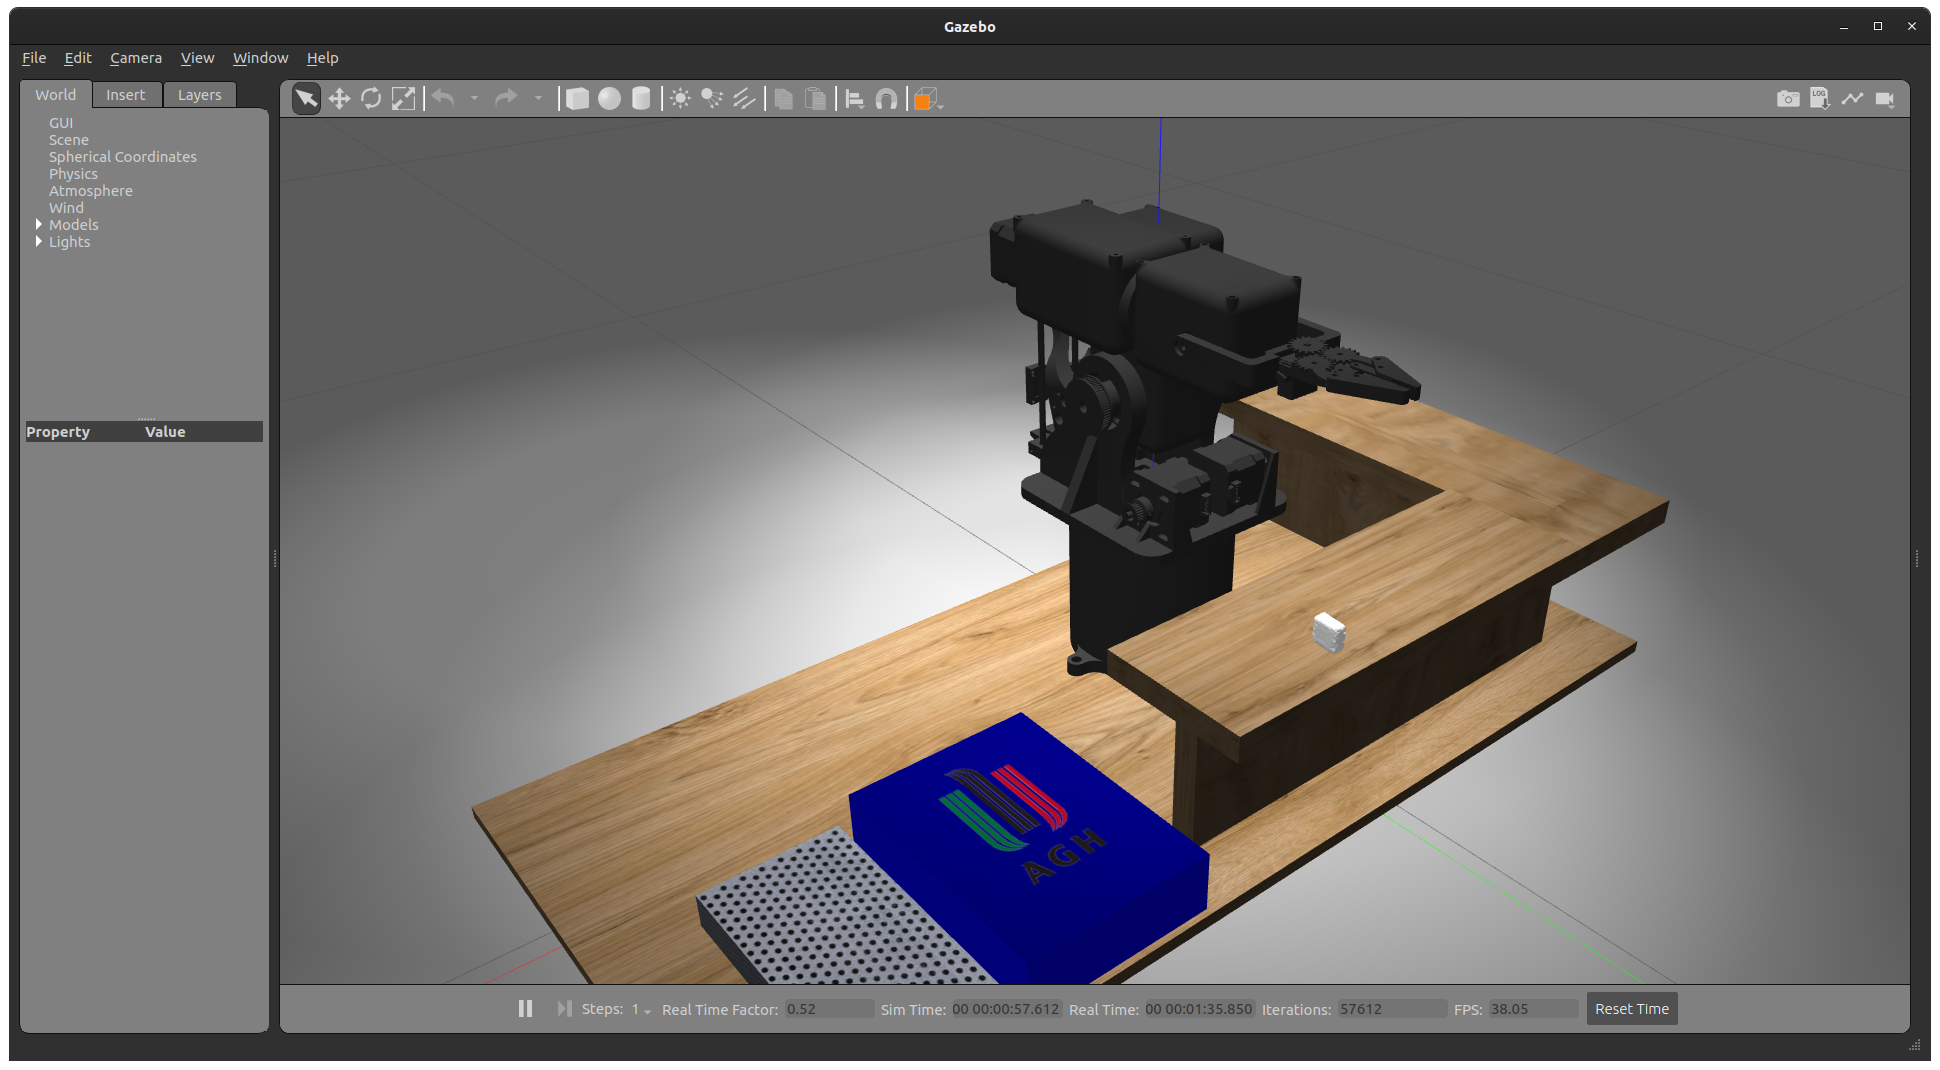
\includegraphics[width=0.9\linewidth]{{img/Bild_gazebo_2.png}}
	\caption{\centering Wirtualny model robota symulowany w środowisku Gazebo. \cite{own}, \cite{oak}, \cite{logo}}
	\label{fig:2}
\end{figure}

Plikiem opisującym importowane środowisko pracy robota, jest format $.world$. Zasadniczo korzystano z domyślnego pustego świata, niemniej na potrzeby późniejszych testów zmodyfikowano go nieco. Dodano niewielki obiekt - kostkę mydła na stoliku przed robotem. Jest ono widoczne na fotografii powyżej - rysunek \ref{fig:2}. \cite{seife_code}

W celu skonfigurowania modelu robota w ROSie posłużono się oprogramowaniem Setup Assistant. Jest to samodzielnie działający pakiet ROSa umożliwiający skonfigurowanie własnego robota i wygenerowanie wszystkich niezbędnych plików do symulowania oraz planowania trajektorii poruszania się manipulatora. Poniższe zdjęcie obrazuje omawiany program - rysunek \ref{fig:9}.

 \begin{figure}[H]
	\centering
	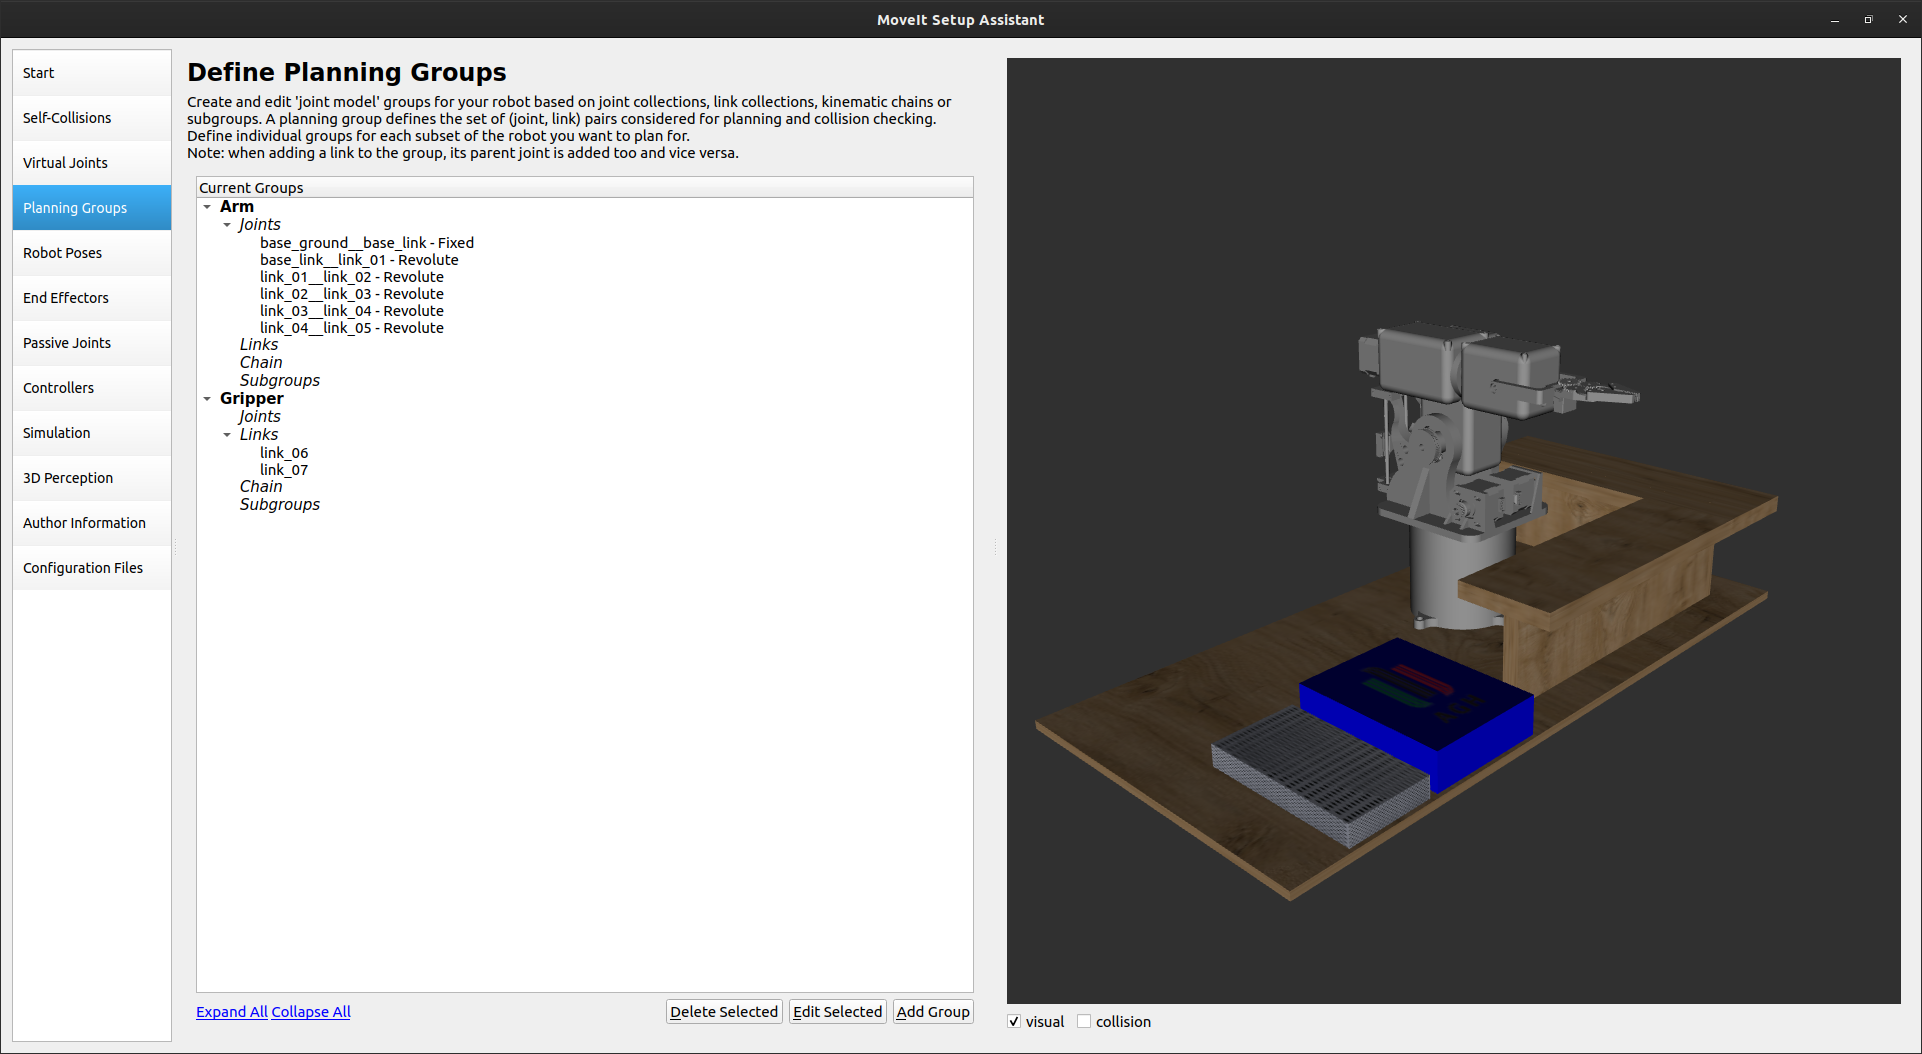
\includegraphics[width=0.9\linewidth]{{img/Bild_SA.png}}
	\caption{\centering Proces konfiguracji robota w programie MoveIt Setup Assistant. \cite{own}, \cite{oak}, \cite{logo}}
	\label{fig:9}
\end{figure}

Jak można zaobserwować z lewej strony powyższego rysunku \ref{fig:9} program ten pozwala na ustawienie wielu parametrów manipulatora. Ustawiono zatem kwestie wzajemnych kolizji jednych elementów robota z innymi. Całą konstrukcję podzielono na dwie grupy złącz. Pierwsza dotyczyła samego ramienia robota, natomiast druga - chwytaka. W dalszej kolejności ustalono charakterystyczne pozycje urządzenia. W tym przypadku pozycja określana jako $home$, to ta w której urządzenie znajduje się po bazowaniu. Zakładka $End$ $Effectors$ związana była z ustawieniami chwytaka - jakie złącza wchodzą w jego skład oraz które jest tak zwanym rodzicem chwytaka, czyli do którego członu jest on przymocowany.

Jedną z najistotniejszych zakładek stanowiła ta odpowiedzialna za konfigurację kontrolerów. To tutaj ustalono jaki planner wykorzystać i jakimi złączami ma sterować. Stworzono dwa kontrolery - jeden dla ramienia oraz drugi dla chwytaka.

Bardzo istotna była także zakładka kolejna, w której możliwe było wygenerowanie pliku $.urdf$ dla symulatora Gazebo.  Plik ten później jeszcze modyfikowano, gdyż dodano do niego fragmenty odpowiedzialne za określanie tekstur obiektów. Ważny jest tutaj fakt, iż Gazebo wymaga osobnych instrukcji opisujących tekstury obiektów aniżeli sam Rviz, który również wczytuje model robota. Toteż konieczne było dodanie fragmentów, które pozwoliły na ich uwzględnienie przez Gazebo. Na koniec wpisywano jeszcze informacje o autorze pracy i ostatecznie generowano automatycznie pliki.

Oczywiście wszystkie skrypty można pisać osobiście, jednak Setup Assistant czyni to znacznie szybciej i przede wszystkim zgodnie ze sztuką. Zatem generuje on niezbędne pliki uruchomieniowe (o rozszerzeniu $.launch$) oraz konfiguracyjne ($.yaml$).

\subsection{Uruchomienie i konfiguracja ROS i MoveIt}

Realizację całego projektu rozpoczęto od pobrania i zainstalowania ROSa. Proces ten należy przeprowadzi w zgodzie z oficjalną instrukcją. Jednak zanim to nastąpiło konieczne było zdecydowanie się na konkretną dystrybucję. W programie wykorzystano ROS Noetic, która jest rekomendowana. Decyzja wyboru dystrybucji nie mogła być bez znaczenia, gdyż występują paczki (specyficzne funkcjonalności), dostępne jedynie pod konkretne dystrybucje. Podobnie nie każda dystrybucja jest dostępna na każdy system operacyjny - było to szczególnie istotne w przypadku Raspberry Pi. Podobnie nie wszystkie dystrybucje wspierają MoveIt. 

Na laptopie, który miał z założenia pełnić role Mastera zainstalowano ROSa w pełnej wersji wraz ze wszystkimi pomocami graficznymi, takimi jak Rviz oraz RQT.


W pierwszej kolejności należało pobrać zawartość repozytorium oprogramowania ROS a następnie odpowiednio go zainstalować. Niezbędne było również dodanie do pliku $~/.bashrc$ informacji o lokalizacji ROSa, tak by otwierając nowe okno terminala, ROS był od razu widoczny.

Dodatek MoveIt zainstalowano z pomocą instrukcji $apt$ $install$, niemniej próbowano także zrealizować to przez tak zwaną instalację ze źródła. W momencie gdy docierano do procesu kompilowania paczek MoveIt pojawiały się liczne błędy. Budowanie udało się dokończyć dopiero na maszynie wirtualnej symulującej Ubuntu 20.04 z zainstalowanym ROSem Noetic. Problemy przy kompilacji jakichkolwiek paczek ROS wynikały z brakujących bibliotek w czasie linkowania, mimo iż biblioteki te były na komputerze zainstalowane. Powodem części niepowodzeń był jednak fakt, że niektórych z bibliotek było więcej (w różnych wersjach) i przez to linker zwracał błędy, nie wiedząc której z nich użyć. Mimo wszystko do końca realizowanego projektu nie udało się w pełni rozwiązać tych problemów, przez co wszystkie kompilacje prowadzono z poziomu dodatkowej maszyny wirtualnej. Jest to o tyle istotne, iż opisywane w poprzednim podrozdziale tworzenie modelu robota w programie Setup Asisstant po wygenerowaniu plików wymagało właśnie kompilacji.

%Tutaj również pojawiały się spore problemy, ze względu na fakt, iż oprogramowanie nie chciało się skompilować. Rzecz ta udała się dopiero na maszynie wirtualnej. W przypadku natywnie zainstalowanego ROS na komputerze osobistym kompilacja kończyła się niepowodzeniem, ze względu na obecne w systemie dwie biblioteki boost w różnych wersjach. Jako iż, biblioteki te były dwie, toteż kompilator 'nie wiedział', którą wybrać przez co zwracał błędy. 

Dysponując już całością koniecznego oprogramowania i stworzonym modelem, możliwe było uruchomienie programu Rviz wraz z dodatkiem MoveIt. Rezultat zaprezentowano poniżej - rysunek \ref{fig:3}.

Oczywiście Rviz nie jest wymagany do planowania i wykonywania trajektorii ruchu robota, gdyż jak to później zostanie przedstawione w rozdziale poświęconym testom, możliwe jest napisanie odpowiedniego skryptu, który zrealizuje to automatycznie. Niemniej wizualizuje on cały proces, co bardzo ułatwia jego zrozumienie. 

Wszystkie funkcje pakietu MoveIt, które można modyfikować z poziomu Rviza, obecne są w lewym dolnym rogu rysunku \ref{fig:3}.

 \begin{figure}[H]
	\centering
	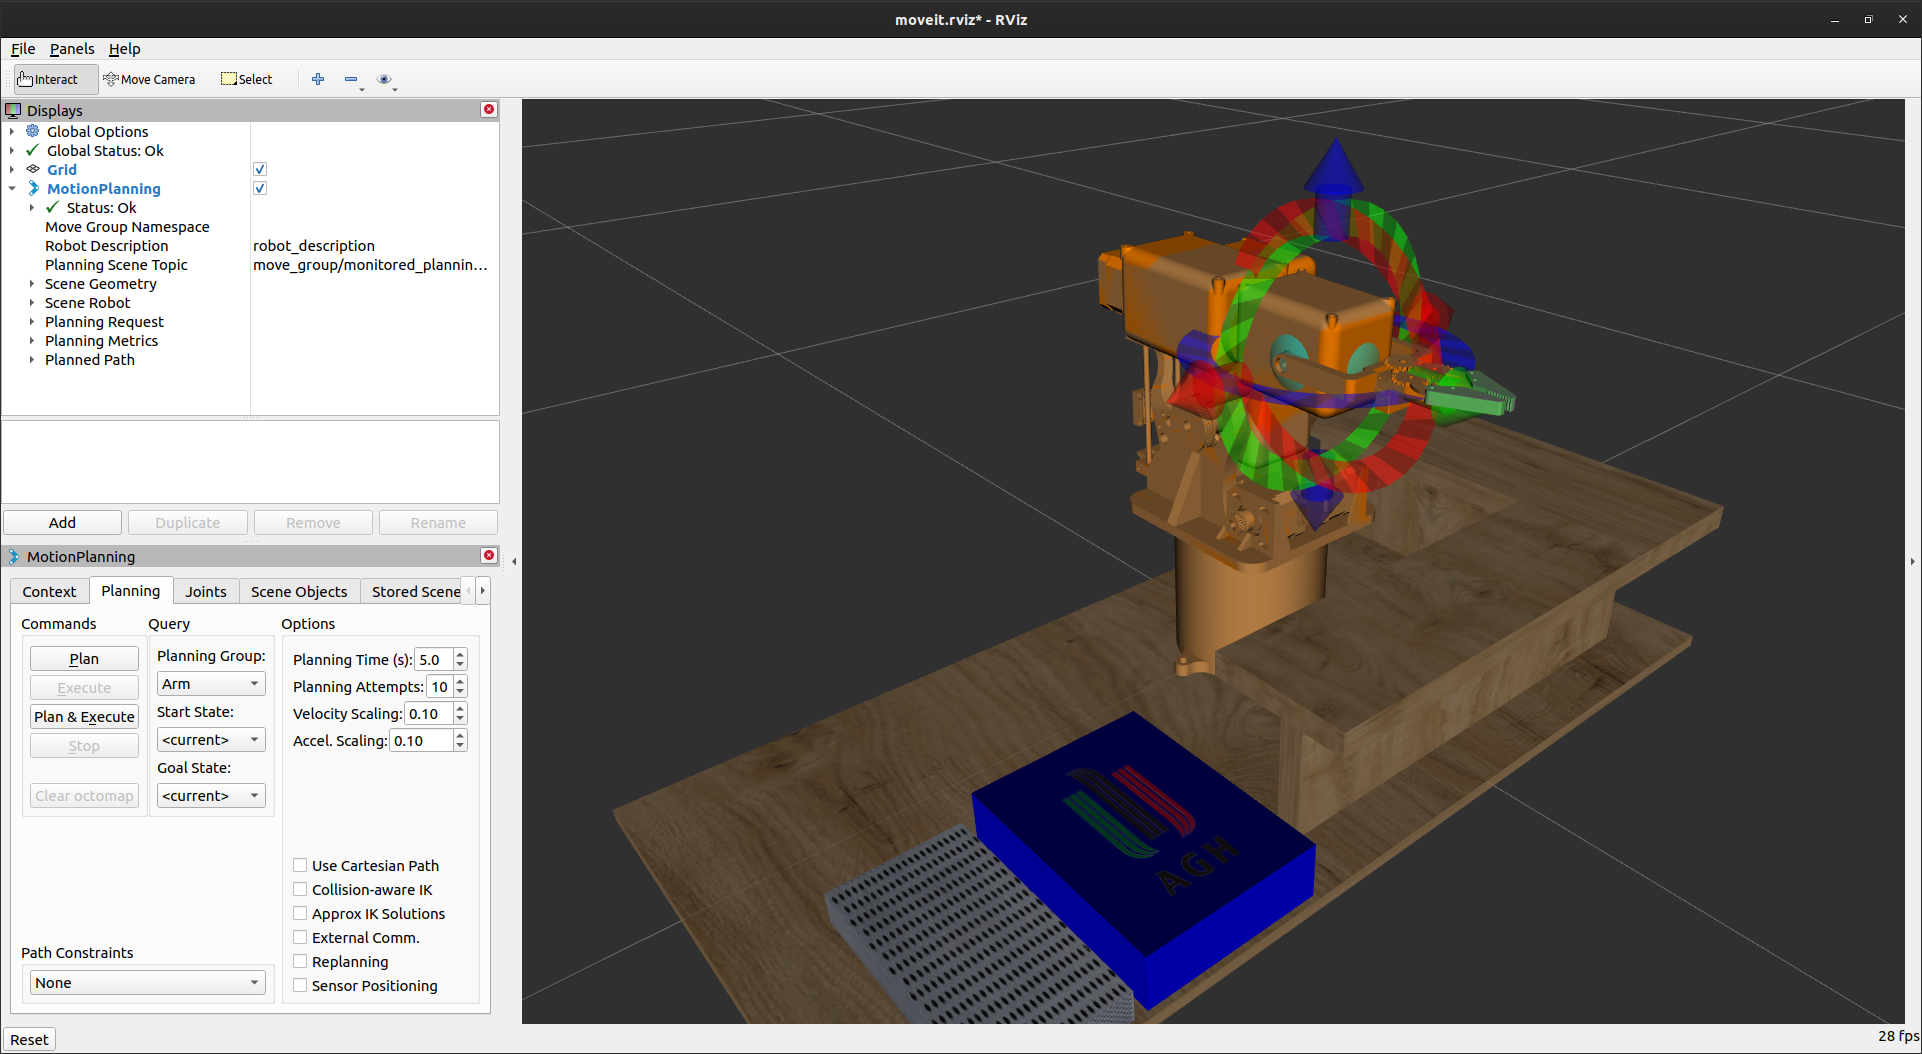
\includegraphics[width=0.9\linewidth]{{img/Bild_rviz.png}}
	\caption{\centering Wirtualny model robota symulowany w środowisku Gazebo. \cite{own}, \cite{oak}, \cite{logo}}
	\label{fig:3}
\end{figure}

Ustalenie nowej pozycji, jaką żądano by robot osiągnął, można było dokonać na dwa sposoby. Pierwszym było poruszanie samym manipulatorem z pomocą widocznych na ramieniu trzecim kolorowych strzałek i pierścieni. Natomiast drugi sposób to ustalenie konkretnych pozycji złącz suwakami w zakładce $joints$.

Istotne jest w przypadku planowania trasy z pomocą MoveIt w programie Rviz zwracanie uwagi na punkt od którego trasa została wyznaczona. Za każdym razem należy wybierać opcję $current$, gdyż w przeciwnym wypadku planowanie nie odbędzie się od obecnej pozycji, tylko poprzedniej, co prowadzi później do niepożądanych sterowań. \cite{ROS_controller_file}

\subsection{Komunikacja zdalna i synchronizacja czasu}

Środowisko ROS umożliwia komunikację ze sobą i współpracę kilku urządzeń - znajdujących się w tej samej sieci lokalnej. Jest to szczególnie przydatne, gdyż moc obliczeniowa jednego komputera może nie być wystarczająca do uruchomienia symulacji np. Gazebo oraz pozostałej funkcjonalności. Stąd też powyższa funkcjonalność.

Autorowi projektu zależało by to komputer na którym jest uruchamiany rdzeń ROS-a, tzw. Master przejmował na siebie większość najważniejszych kwestii związanych chociażby z planowaniem oraz symulacją. Natomiast mikrokontroler Raspberry Pi4B stanowił jedynie łącznik, na który odbierał sygnały z Mastera i z pomocą portów USB komunikował się mikrokontrolerami wykonawczymi STM i ESP. Istniała co prawda możliwość sterowania stepstickami robota bezpośrednio z poziomu Raspberry, niemniej dla zabezpieczenia się przed ewentualnymi uszkodzeniami, pozostawiono STM32.

Przy czym kod źródłowy mikrokontrolera STM32 również wymagał wprowadzenia zmian, w związku z koniecznością odbierania wiadomości od RPi4B. Zatem jego oprogramowanie zmodyfikowano o odczyt z pomocą DMA informacji przychodzących z USB, po czym wyciąganie z nich zarówno prędkości każdego z silnika, jak i ilości kroków do wykonania. 

W celu uruchomienia ROSa na różnych urządzeniach wystarczy dokonać wpisu do pliku konfiguracyjnego $~/.bashrc$. Wystarczy dodać niniejszą instrukcję na komputerze Mastera:

\begin{minted}{bash}
# ~/.bashrc: executed by bash(1) for non-login shells.
# [...]
export ROS_MASTER_URI=http://192.168.0.103:11311 # IP laptopa
export ROS_IP=192.168.0.103 # IP laptopa
# [...]
\end{minted}

Oraz na pozostałych urządzeniach:

\begin{minted}{bash}
# ~/.bashrc: executed by bash(1) for non-login shells.
# [...]
export ROS_MASTER_URI=http://192.168.0.103:11311 # IP laptopa
export ROS_IP=192.168.0.101 # IP Raspberry Pi
# [...]
\end{minted}

Po sprzężeniu ze sobą komputera i Rasberry okazało się, iż niezbędne jest jeszcze uruchomienie synchronizacji między dwoma urządzeniami. W przeciwnym wypadku ROS zwracał ostrzeżenia o nieaktualnych pozycjach złącz. W tym celu uruchomiono na laptopie serwer czasu NTP, a na mikrokomputerze jego klienta. Skorzystano z protokołu Chrony. Po zainstalowaniu programu Chronyd na obu urządzeniach, niezbędne było przeprowadzenie konfiguracji systemu w plikach ustawieniowych ($/etc/chrony.conf $). W laptopie należało podać adres IP urządzeń, którym zezwala się podłączyć do synchronizatora czasu (wpis $allow$ $192.168.0.103$). Natomiast w RPi4B adres serwera (wpis $server$ $192.168.0.101$).

 \begin{figure}[H]
	\centering
	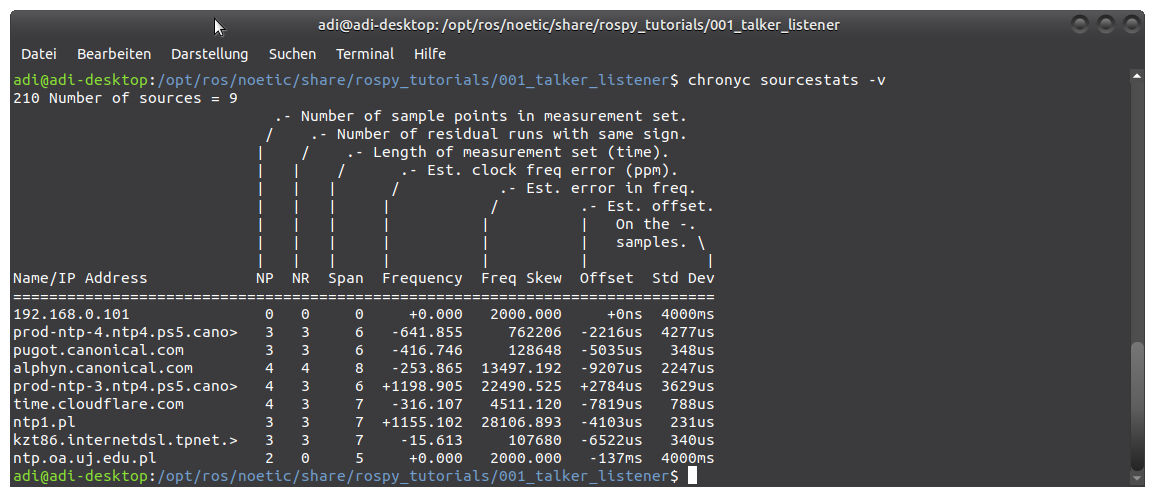
\includegraphics[width=1\linewidth]{{img/Bild_chrony.png}}
	\caption{ \centering Włączona synchronizacja czasu na Raspberry Pi. \cite{own}}
	\label{fig:46}
\end{figure}

Na obrazie powyżej ukazano terminal mikrokomputera Raspberry Pi z wywołaną komendą odpowiedzialną za wyświetlenie informacji na temat aktywnej synchronizacji czasu. Na pierwszej pozycji od góry tabeli widoczny jest adres laptopa, czyli przypisanego serwera. Podobnie laptop rozpoznaje podpiętych klientów - rysunek \ref{fig:47}{}

 \begin{figure}[H]
	\centering
	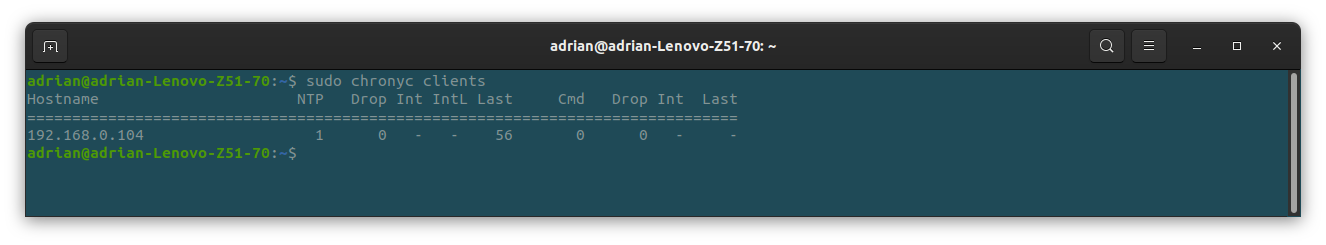
\includegraphics[width=1\linewidth]{{img/Bild_chrony_laptop.png}}
	\caption{ \centering Włączona synchronizacja czasu na laptopie. \cite{own}}
	\label{fig:47}
\end{figure}

Jak widać adres IP na obrazie ma końcówkę 104, co wynika z faktu, iż nie przypisywano temu Raspberry Pi stałego adresu, toteż czasami zmienia się on w zależności od ilości podpiętych do domowej sieci urządzeń.

Poniżej zaprezentowano (obraz \ref{fig:44}) proces testowania działania komunikacji między laptopem oraz Raspberry Pi. Na zdjęciu widoczny jest ekran laptopa na którym uruchomiono rdzeń ROS wraz z MoveItem w programie Rviz. Natomiast monitor wyświetla obraz z Raspberry Pi (widniejący ekran powitalny systemu Ubuntu Mate 20.04). W terminalach obu maszyn wywołano instrukcję $rostopic$ $list$, dzięki temu uzyskano potwierdzenie, iż komunikacja sieciowa działa. Dodatkowo na mikrokomputerze uruchomiono także program odpowiedzialny za wysyłanie stanu enkoderów, toteż widoczne jest, iż wirtualna pozycja robota odpowiada tej rzeczywistej.

 \begin{figure}[H]
	\centering
	\includegraphics[width=0.9\linewidth]{{img/Bild_all_robot.jpg}}
	\caption{ \centering Testy komunikacji między systemami i poprawności funkcjonowania enkoderów. \cite{own}, \cite{oak}}
	\label{fig:44}
\end{figure}

Na obrazie widoczny jest także sam mikrokomputer Raspberry Pi, w charakterystycznej, wydrukowanej czarnej obudowie z wentylatorem.

\section{Podsumowanie rozdziału}

Podsumowując zaprezentowane w niniejszym rozdziale prace można stwierdzić, iż realizowany projekt kontrolera był dosyć złożony. Wymagane były umiejętności w różnych dziedzinach. Wiele rzeczy realizowano po raz pierwszy przez co konieczne było zmaganie się z licznymi błędami. W czasie realizacji projektu uszkodzono także serwomotor odpowiedzialny za chwytak. Konieczna była jego wymiana. Podobnie awarii uległa karta pamięci w mikrokomputerze Raspberry Pi. Gdyby nie kopia projektu na repozytorium, wówczas cały program należałoby pisać od początku. Podobnie też wiele połączeń lutowanych musiano poprawiać, gdyż często się łamały pod wpływem ruchu robota bądź nie stykały jak powinny. Zatem wnioski jakie się nasuwają od strony technicznej to konieczność zabezpieczania swoich prac i bycia świadomym licznych niepowodzeń, a także zniszczeń.

Podobnie materiał z jakiego wydrukowano robota - PLA, źle znosi promieniowanie UV. Elementy robota, które w czasie realizacji projektu inżynierskiego pasowano ciasno na wcisk, okazywały się po czasie być luźne. Elementy minimalnie zmieniły swoje wymiary.

Realizacja projektu okraszona była także licznymi dodatkowymi zmianami i modyfikacjami, których jednak nie wymieniono w powyższym opisie. Często chęć zaimplementowania najprostszej funkcji wiązała się z wielogodzinnym poszukiwaniem rozwiązania, a zdarzały się sytuacje kiedy to po całym dniu okazywało się, iż dana funkcjonalność nie występuje.  

	\chapter{Testowanie i eksperymenty}

Testowanie, porównywanie sposobu działania poszczególnych plannerów a także tworzenie różnych próbnych scenariuszy stanowiło najważniejszy cel realizowanego projektu. To wszystko miało służyć wykreowaniu swoistego oglądu sytuacji jakie sposoby kontroli są najoptymalniejsze, jakie nadają się do konkretnych zastosowań, a także co składa się na ich słabe strony. Przeprowadzone testy miały służyć również zobrazowaniu możliwości MoveIta. W tym celu zaproponowano szereg eksperymentów, których wyniki zestawiono w poniższych podrozdziałach. By móc zbierać konkretne pomiary napisano w tym celu kilka skryptów w języku Python. Byli to klasyczni subskrybenci ROS, którzy zapisywali pożądane wartości do plików csv. W dalszej kolejności na ich podstawie generowano wykresy, tabele itp.

\section{Porównanie planerów}

\subsection{Czas planowania}
Jednym z pierwszych testów jakie przeprowadzono było porównanie czasów planowania trasy przez poszczególne plannery. W tym celu przygotowano dwa osobne scenariusze. W pierwszym z nich trasa do pokonania była bardzo prosta. Robot musiał poruszyć jedynie jednym złączem. Planowanie trasy dla każdego algorytmu powtarzano 10 krotnie, tak by na końcu móc policzyć średni czas procesu. Wielokrotne pomiary miały na celu pominięcie kwestii możliwego chwilowego obciążenia komputera wskutek wykonywania np. obsługiwanego przerwania. Kolejną rzeczą jest, iż czas planowania będzie różny przy wykorzystaniu innego komputera do obliczeń, niemniej różnice między plannerami pozostaną.

Poniższa tabela \ref{tab:10} prezentuje zebrane dane. Każdy algorytm miał do wyznaczenia trasę od pozycji pobazowej (wszystkie złącza 0$^\circ$) do pozycji w której ramię drugie opuszczone było o 35$^\circ$. Pozostałe złącza bez zmian.
 Należy podkreślić, iż eksperymenty te były prowadzone na domyślnych ustawieniach plannerów wygenerowanych przez program Setup Assistant. Dozwolona ilość podejść algorytmu do wyznaczenia trasy wynosiła 10. Pomiary wykonano na laptopie Lenovo Z51 z procesorem Intel i7 5500U, 8GB RAM DDR3, dyskiem SSD 1 TB Samsung QVO 870. Zainstalowany system jak wcześniej informowano to Ubuntu 20.04. W czasie testów nie były uruchomione inne zasobożerne procesy - jedynie notatnik do zapisywania pomiarów.   
% Please add the following required packages to your document preamble:
% \usepackage{multirow}
% \usepackage[table,xcdraw]{xcolor}
% If you use beamer only pass "xcolor=table" option, i.e. \documentclass[xcolor=table]{beamer}
\begin{table}[H]
\centering
\caption{Zestawienie czasów planowania ruchu ramienia drugiego przez poszczególne algorytmy}
\label{tab:10}
\begin{tabular}{|c|c|c|c|c|c|ll}
\cline{1-6}
\cellcolor[HTML]{C0C0C0}L.p. & \multicolumn{1}{l|}{\cellcolor[HTML]{C0C0C0}{\color[HTML]{000000} \begin{tabular}[c]{@{}l@{}}Grupa \\ plannerów\end{tabular}}} & \cellcolor[HTML]{C0C0C0}Planner     & \cellcolor[HTML]{C0C0C0}\begin{tabular}[c]{@{}c@{}}Min. czas\\ planowania {[}s{]}\end{tabular} & \cellcolor[HTML]{C0C0C0}\begin{tabular}[c]{@{}c@{}}Max. czas\\ planowania {[}s{]}\end{tabular} & \cellcolor[HTML]{C0C0C0}\begin{tabular}[c]{@{}c@{}}Średni czas \\ 10 prób {[}s{]}\end{tabular} &  &  \\ \cline{1-6}
\cellcolor[HTML]{EFEFEF}1.   & CHOMP                                                                                                                          & \cellcolor[HTML]{EFEFEF}CHOMP       & \cellcolor[HTML]{EFEFEF}0.253                                                                  & \cellcolor[HTML]{EFEFEF}0.313                                                                  & \cellcolor[HTML]{EFEFEF}0.267                                                                  &  &  \\ \cline{1-6}
\cellcolor[HTML]{C0C0C0}2.   &                                                                                                                                & \cellcolor[HTML]{C0C0C0}BFMT        & \cellcolor[HTML]{C0C0C0}1.164                                                                  & \cellcolor[HTML]{C0C0C0}0.959                                                                  & \cellcolor[HTML]{C0C0C0}1.027                                                                  &  &  \\ \cline{1-1} \cline{3-6}
\cellcolor[HTML]{FFCCC9}3.   &                                                                                                                                & \cellcolor[HTML]{FFCCC9}BKPIECE     & \cellcolor[HTML]{FFCCC9}2.565                                                                  & \cellcolor[HTML]{FFCCC9}-                                                                      & \cellcolor[HTML]{FFCCC9}2.565                                                                  &  &  \\ \cline{1-1} \cline{3-6}
\cellcolor[HTML]{9AFF99}4.   &                                                                                                                                & \cellcolor[HTML]{9AFF99}BiEST       & \cellcolor[HTML]{9AFF99}0.037                                                                  & \cellcolor[HTML]{9AFF99}0.048                                                                  & \cellcolor[HTML]{9AFF99}0.042                                                                  &  &  \\ \cline{1-1} \cline{3-6}
\cellcolor[HTML]{9AFF99}5.   &                                                                                                                                & \cellcolor[HTML]{9AFF99}BiTRRT      & \cellcolor[HTML]{9AFF99}0.020                                                                  & \cellcolor[HTML]{9AFF99}0.029                                                                  & \cellcolor[HTML]{9AFF99}0.023                                                                  &  &  \\ \cline{1-1} \cline{3-6}
\cellcolor[HTML]{C0C0C0}6.   &                                                                                                                                & \cellcolor[HTML]{C0C0C0}EST         & \cellcolor[HTML]{C0C0C0}0.070                                                                  & \cellcolor[HTML]{C0C0C0}0.185                                                                  & \cellcolor[HTML]{C0C0C0}0.121                                                                  &  &  \\ \cline{1-1} \cline{3-6}
\cellcolor[HTML]{EFEFEF}7.   &                                                                                                                                & \cellcolor[HTML]{EFEFEF}FMT         & \cellcolor[HTML]{EFEFEF}0.892                                                                  & \cellcolor[HTML]{EFEFEF}0.965                                                                  & \cellcolor[HTML]{EFEFEF}0.925                                                                  &  &  \\ \cline{1-1} \cline{3-6}
\cellcolor[HTML]{C0C0C0}8.   &                                                                                                                                & \cellcolor[HTML]{C0C0C0}KPIECE      & \cellcolor[HTML]{C0C0C0}0.109                                                                  & \cellcolor[HTML]{C0C0C0}0.270                                                                  & \cellcolor[HTML]{C0C0C0}0.155                                                                  &  &  \\ \cline{1-1} \cline{3-6}
\cellcolor[HTML]{FFCCC9}9.   &                                                                                                                                & \cellcolor[HTML]{FFCCC9}LBKPIECE    & \cellcolor[HTML]{FFCCC9}X                                                                      & \cellcolor[HTML]{FFCCC9}X                                                                      & \cellcolor[HTML]{FFCCC9}X                                                                      &  &  \\ \cline{1-1} \cline{3-6}
\cellcolor[HTML]{C0C0C0}10.  &                                                                                                                                & \cellcolor[HTML]{C0C0C0}LBTRRT      & \cellcolor[HTML]{C0C0C0}0.102                                                                  & \cellcolor[HTML]{C0C0C0}-                                                                      & \cellcolor[HTML]{C0C0C0}0.102                                                                  &  &  \\ \cline{1-1} \cline{3-6}
\cellcolor[HTML]{FFCCC9}11.  &                                                                                                                                & \cellcolor[HTML]{FFCCC9}LazyPRM     & \cellcolor[HTML]{FFCCC9}X                                                                      & \cellcolor[HTML]{FFCCC9}X                                                                      & \cellcolor[HTML]{FFCCC9}X                                                                      &  &  \\ \cline{1-1} \cline{3-6}
\cellcolor[HTML]{C0C0C0}12.  &                                                                                                                                & \cellcolor[HTML]{C0C0C0}LazyPRMstar & \cellcolor[HTML]{C0C0C0}0.101                                                                  & \cellcolor[HTML]{C0C0C0}-                                                                      & \cellcolor[HTML]{C0C0C0}0.101                                                                  &  &  \\ \cline{1-1} \cline{3-6}
\cellcolor[HTML]{EFEFEF}13.  &                                                                                                                                & \cellcolor[HTML]{EFEFEF}PDST        & \cellcolor[HTML]{EFEFEF}0.071                                                                  & \cellcolor[HTML]{EFEFEF}0.228                                                                  & \cellcolor[HTML]{EFEFEF}0.138                                                                  &  &  \\ \cline{1-1} \cline{3-6}
\cellcolor[HTML]{C0C0C0}14.  &                                                                                                                                & \cellcolor[HTML]{C0C0C0}PRM         & \cellcolor[HTML]{C0C0C0}0.057                                                                  & \cellcolor[HTML]{C0C0C0}0.119                                                                  & \cellcolor[HTML]{C0C0C0}0.085                                                                  &  &  \\ \cline{1-1} \cline{3-6}
\cellcolor[HTML]{EFEFEF}15.  &                                                                                                                                & \cellcolor[HTML]{EFEFEF}PRMstar     & \cellcolor[HTML]{EFEFEF}0.101                                                                  & \cellcolor[HTML]{EFEFEF}-                                                                      & \cellcolor[HTML]{EFEFEF}0.101                                                                  &  &  \\ \cline{1-1} \cline{3-6}
\cellcolor[HTML]{C0C0C0}16.  &                                                                                                                                & \cellcolor[HTML]{C0C0C0}ProjEST     & \cellcolor[HTML]{C0C0C0}0.064                                                                  & \cellcolor[HTML]{C0C0C0}0.197                                                                  & \cellcolor[HTML]{C0C0C0}0.139                                                                  &  &  \\ \cline{1-1} \cline{3-6}
\cellcolor[HTML]{9AFF99}11.  &                                                                                                                                & \cellcolor[HTML]{9AFF99}RRTConnect  & \cellcolor[HTML]{9AFF99}0.22                                                                   & \cellcolor[HTML]{9AFF99}0.046                                                                  & \cellcolor[HTML]{9AFF99}0.036                                                                  &  &  \\ \cline{1-1} \cline{3-6}
\cellcolor[HTML]{C0C0C0}12.  &                                                                                                                                & \cellcolor[HTML]{C0C0C0}RRT         & \cellcolor[HTML]{C0C0C0}0.032                                                                  & \cellcolor[HTML]{C0C0C0}0.080                                                                  & \cellcolor[HTML]{C0C0C0}0.516                                                                  &  &  \\ \cline{1-1} \cline{3-6}
\cellcolor[HTML]{EFEFEF}13.  &                                                                                                                                & \cellcolor[HTML]{EFEFEF}RRTstar     & \cellcolor[HTML]{EFEFEF}0.101                                                                  & \cellcolor[HTML]{EFEFEF}-                                                                      & \cellcolor[HTML]{EFEFEF}0.101                                                                  &  &  \\ \cline{1-1} \cline{3-6}
\cellcolor[HTML]{FFCCC9}14.  &                                                                                                                                & \cellcolor[HTML]{FFCCC9}SBL         & \cellcolor[HTML]{FFCCC9}2.011                                                                  & \cellcolor[HTML]{FFCCC9}-                                                                      & \cellcolor[HTML]{FFCCC9}2.011                                                                  &  &  \\ \cline{1-1} \cline{3-6}
\cellcolor[HTML]{EFEFEF}15.  &                                                                                                                                & \cellcolor[HTML]{EFEFEF}SPARS       & \cellcolor[HTML]{EFEFEF}0.183                                                                  & \cellcolor[HTML]{EFEFEF}-                                                                      & \cellcolor[HTML]{EFEFEF}0.183                                                                  &  &  \\ \cline{1-1} \cline{3-6}
\cellcolor[HTML]{C0C0C0}16.  &                                                                                                                                & \cellcolor[HTML]{C0C0C0}SPARStwo    & \cellcolor[HTML]{C0C0C0}0.101                                                                  & \cellcolor[HTML]{C0C0C0}-                                                                      & \cellcolor[HTML]{C0C0C0}0.101                                                                  &  &  \\ \cline{1-1} \cline{3-6}
\cellcolor[HTML]{EFEFEF}17.  &                                                                                                                                & \cellcolor[HTML]{EFEFEF}STRIDE      & \cellcolor[HTML]{EFEFEF}0.081                                                                  & \cellcolor[HTML]{EFEFEF}0.175                                                                  & \cellcolor[HTML]{EFEFEF}0.118                                                                  &  &  \\ \cline{1-1} \cline{3-6}
\cellcolor[HTML]{9AFF99}18.  & \multirow{-23}{*}{OMPL}                                                                                                        & \cellcolor[HTML]{9AFF99}TRRT        & \cellcolor[HTML]{9AFF99}0.022                                                                  & \cellcolor[HTML]{9AFF99}0.047                                                                  & \cellcolor[HTML]{9AFF99}0.033                                                                  &  &  \\ \cline{1-6}
\cellcolor[HTML]{9AFF99}19.  &                                                                                                                                & \cellcolor[HTML]{9AFF99}PTP         & \cellcolor[HTML]{9AFF99}0.000                                                                  & \cellcolor[HTML]{9AFF99}0.001                                                                  & \cellcolor[HTML]{9AFF99}0.001                                                                  &  &  \\ \cline{1-1} \cline{3-6}
\cellcolor[HTML]{9AFF99}20.  & \multirow{-2}{*}{\begin{tabular}[c]{@{}c@{}}Pilz Industrial \\ Motion Planner\end{tabular}}                                    & \cellcolor[HTML]{9AFF99}LIN         & \cellcolor[HTML]{9AFF99}0.004                                                                  & \cellcolor[HTML]{9AFF99}0.007                                                                  & \cellcolor[HTML]{9AFF99}0.005                                                                  &  &  \\ \cline{1-6}
\end{tabular}
\end{table}
Wnioski jakie nasuwają się po przeanalizowaniu powyższego zestawienia to fakt, iż różnice w czasach planowania istotnie występują. Wiele plannerów osiąga zbliżone czasy, natomiast część znacząco odbiega od pozostałych. 

Dla prostego zadania, jakim było poruszenie jednym złączem grupa plannerów wchodzących w skład Pilz Industrial Motion Planner wydaje się być bezkonkurencyjna. Ścieżkę otrzymywano praktycznie natychmiast. Ze względu na opisywaną w rozdziale drugim prostotę tych algorytmów świetnie nadają się one do takowych zastosowań. 

Najlepsze z algorytmów wchodzących w skład grupy OMPL również okazały się całkiem szybkie. Planowanie trasy zajmowało średnio od dwóch do czterech setnych sekundy. 

Dziwi natomiast fakt, iż plannery takie jak LBKPIECE oraz LazyPRM nie były w stanie w ogóle zaplanować trasy. Pierwszy z wymienionych spowodował zawieszenie się programu Rviz (prawdopodobnie wystąpił błąd). Natomiast w drugim przypadku pomimo zwiększenia maksymalnego czasu planowania do 60 sekund - wyniku nie otrzymano.

W przeprowadzonych eksperymentach bardzo źle wypadł również planner BKPIECE. Najniższy odnotowany czas planowania (ponad 2.5 sekundy) udało się zaobserwować tylko raz. Pozostałe czasy przekraczały zazwyczaj dwukrotnie tę wartość. Dodatkowo bardzo często przy wybraniu zbyt niskiej maksymalnej długości czasu planowania, zabieg ten w ogóle się nie udawał. Planowanie trajektorii kończyło się błędem (nie znajdowano trasy w dopuszczalnym czasie). 

Zauważono, że algorytmy posiadające w nazwie człon $star$ (chociaż nie tylko) charakteryzowało specyficzne zachowanie. Wykorzystywały one cały określony przez użytkownika maksymalny czas planowania, próbując znaleźć najlepsze możliwe rozwiązanie. Dopiero po upływie tego czasu wybierały optymalną znalezioną trajektorię. Często minimalny potrzebny do zaplanowania czas wynosił jedną dziesiątą sekundy (czyli minimum możliwe do ustalenia w Rviz), niemniej zdarzało się, iż potrzebowały one tego czasu więcej (np. algorytm SBL, który potrzebował minimum 2 sekund na znalezienie trasy). W takich przypadkach nie należy opierać swoich założeń, o wyznaczony minimalny czas, gdyż nie jest on powtarzalny. Oznacza to, iż przykładowo na dziesięć prób, raz uda się uzyskać taki czas, natomiast w pozostałych przypadkach proces zakończy się niepowodzeniem. Dlatego w praktyce minimalny czas dający gwarancję otrzymania wyniku będzie dwu lub nawet trzykrotnie większy.

Zauważono również, iż w przypadku plannera CHOMP, mimo umiarkowanych czasów planowania jakie otrzymywano, cały proces od momentu jego uruchomienia do zwrócenia wyniku był znacząco dłuższy od wskazywanego. Odnosi się zatem wrażenie jakoby spore znaczenie miało również wywołanie i obsługa plannera, a nie tylko sam proces działania algorytmu wyznaczającego trasę. W przypadku plannerów OMPL i Pilz nie zaobserwowano takiej tendencji.

%Dzieje się tak, ze względu na sposób ustalania minimalnego czasu planowania dla takich algorytmów. Stosowano system 10 prób. Jeżeli dla zadanego czasu maksymalnego planowania (np. 2 sekund) dziesięć razy z rzędu wyznaczanie trasy kończyło się niepowodzeniem, wówczas uznawano, iż algorytm nie jest w stanie zaplanować ruchu w tak krótkim czasie. 



W dalszej kolejności postanowiono powtórzyć test jednak z uwzględnieniem konieczności przemieszczenia wszystkich złącz. Chciano w ten sposób sprawdzić czy dla plannera ma znaczenie ile osi musi ustawić. Jednak w tym eksperymencie postanowiono pominąć już algorytmy, które w poprzednim zestawieniu wypadły najsłabiej. 

Wyniki zaprezentowano poniżej (wykres \ref{fig:30}), zestawiając ze sobą średni czas 10 prób przy planowaniu ruchu jednej oraz wszystkich osi. W ten sposób możliwe jest zaobserwowanie ewentualnej różnicy. Pomiary dla jednej osi zaczerpnięto z poprzedniego eksperymentu (\ref{tab:4}). Natomiast w przypadku pomiarów wszystkich osi, ich nastawy były kolejno: 90$^\circ$ wieża, -10$^\circ$ ram. główne, -20$^\circ$ ram. drugie, 90$^\circ$ ram. trzecie, 30$^\circ$ obrót chwytaka. W każdym przypadku dozwolona ilość podejść algorytmu do wyznaczenia trasy wynosiła 10. 

 \begin{figure}[H]
	\centering
	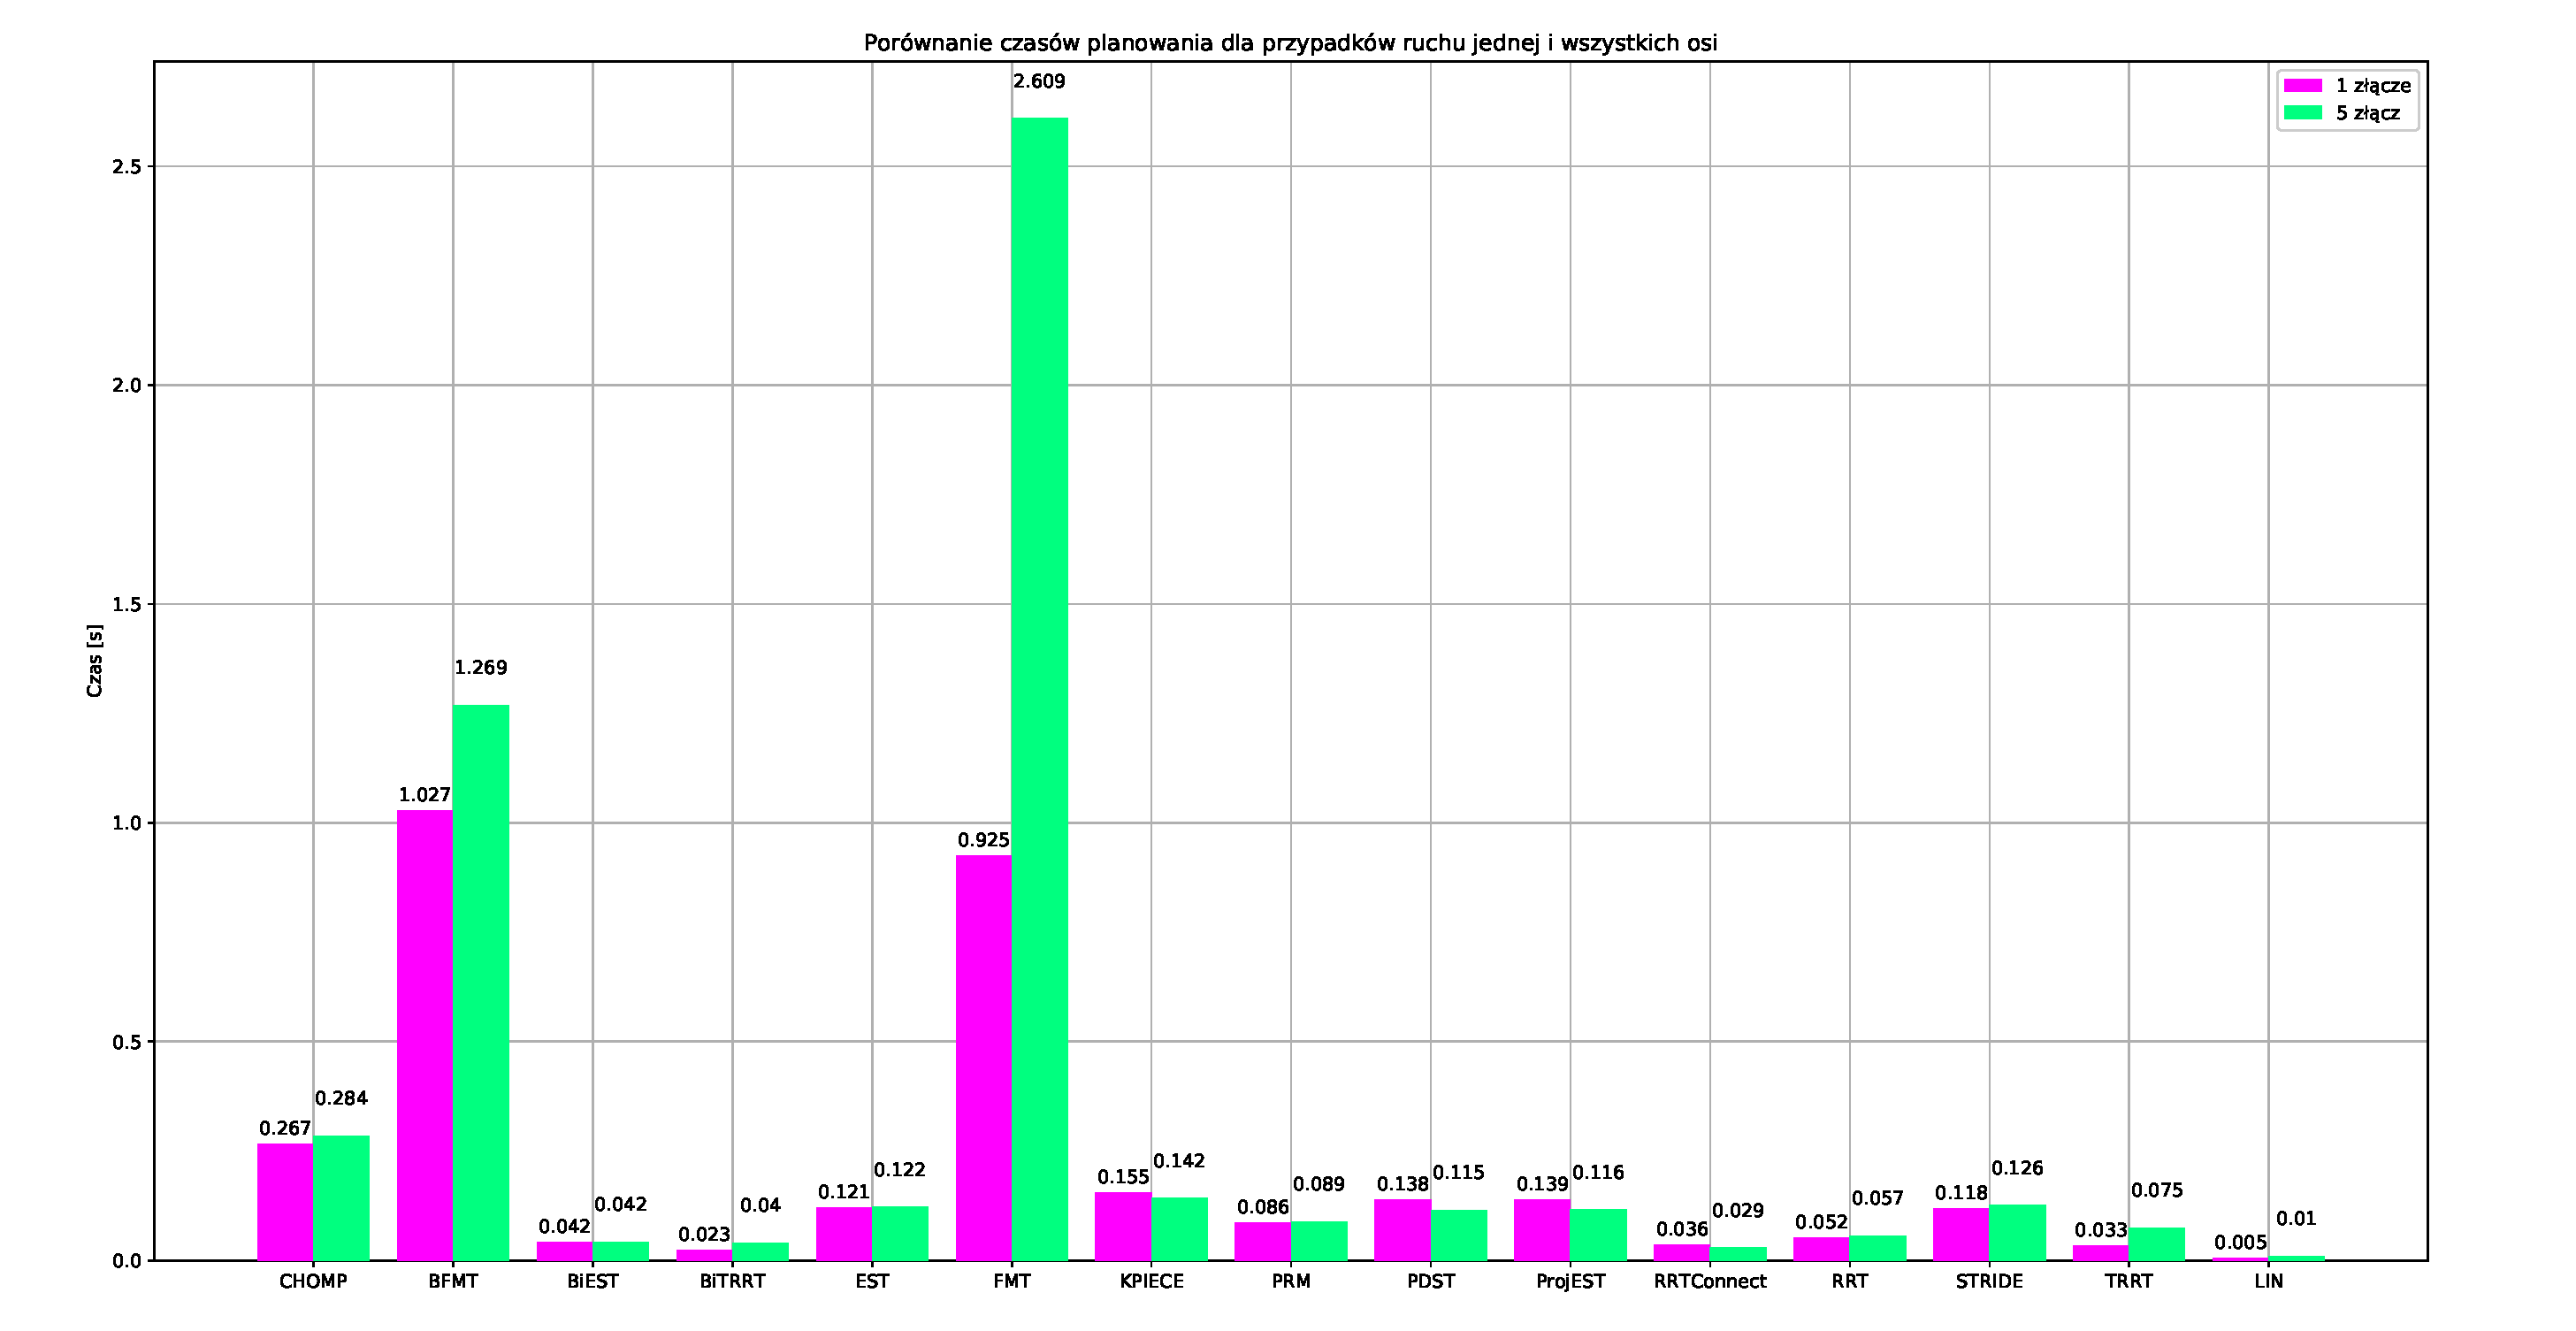
\includegraphics[width=0.9\linewidth]{{img/Figure_com.eps}}
	\caption{Porównanie czasów planowania dla przypadku ruchu jednej i wszystkich osi.}
	\label{fig:30}
\end{figure}

Powyższy wykres uwidacznia fakt, iż zasadniczo dla dwóch plannerów - BFMT oraz FMT ma znaczenie ile członów robota muszą przemieścić. Szczególnie w przypadku algorytmu FMT różnica jest ogromna. Względnie dużą zmianę odnotowano także w przypadku algorytmów BiEST, BiTRRT, TRRT oraz LIN. Mimo nawet dwukrotnemu wydłużeniu procesu planowania, czasy przez nie uzyskiwane nadal pozostają na bardzo dobrym poziomie. Natomiast jeżeli chodzi o pozostałe plannery, to różnice są raczej niewielkie. Czasami wręcz na korzyść wszystkich złącz, niemniej na tyle subtelne, iż raczej nie stwierdzano by na ich podstawie jednoznacznej tendencji. Warto również zaznaczyć, iż w porównaniu nie uwzględniono algorytmu Pilz PTP, gdyż w jego sytuacji nie odnotowano żadnej różnicy w czasie wyznaczania trasy.

Jak wcześniej informowano - wszystkie dotychczas przeprowadzane eksperymenty dotyczyły sytuacji dla 10 dozwolonych prób planowania trasy przez algorytm. Postanowiono zatem sprawdzić jak dopuszczalna ilość tych prób przekłada się na czas wygenerowania trasy. 

Wyniki zestawiono na poniższym wykresie słupkowym. Jak wcześniej pominięto niektóre z najsłabszych algorytmów oraz te wykorzystujące cały dopuszczalny czas planowania. Sprawdzano czasy planowania dla ograniczenia 1 podejścia, 10 oraz 20. Jak i poprzednio każda z zaprezentowanych na zestawieniu wartości stanowi średnią z 10 różnych pomiarów. Przemieszczenie złącz było identyczne jak w poprzednim teście - wymagany ruch wszystkich osi robota.

 \begin{figure}[H]
	\centering
	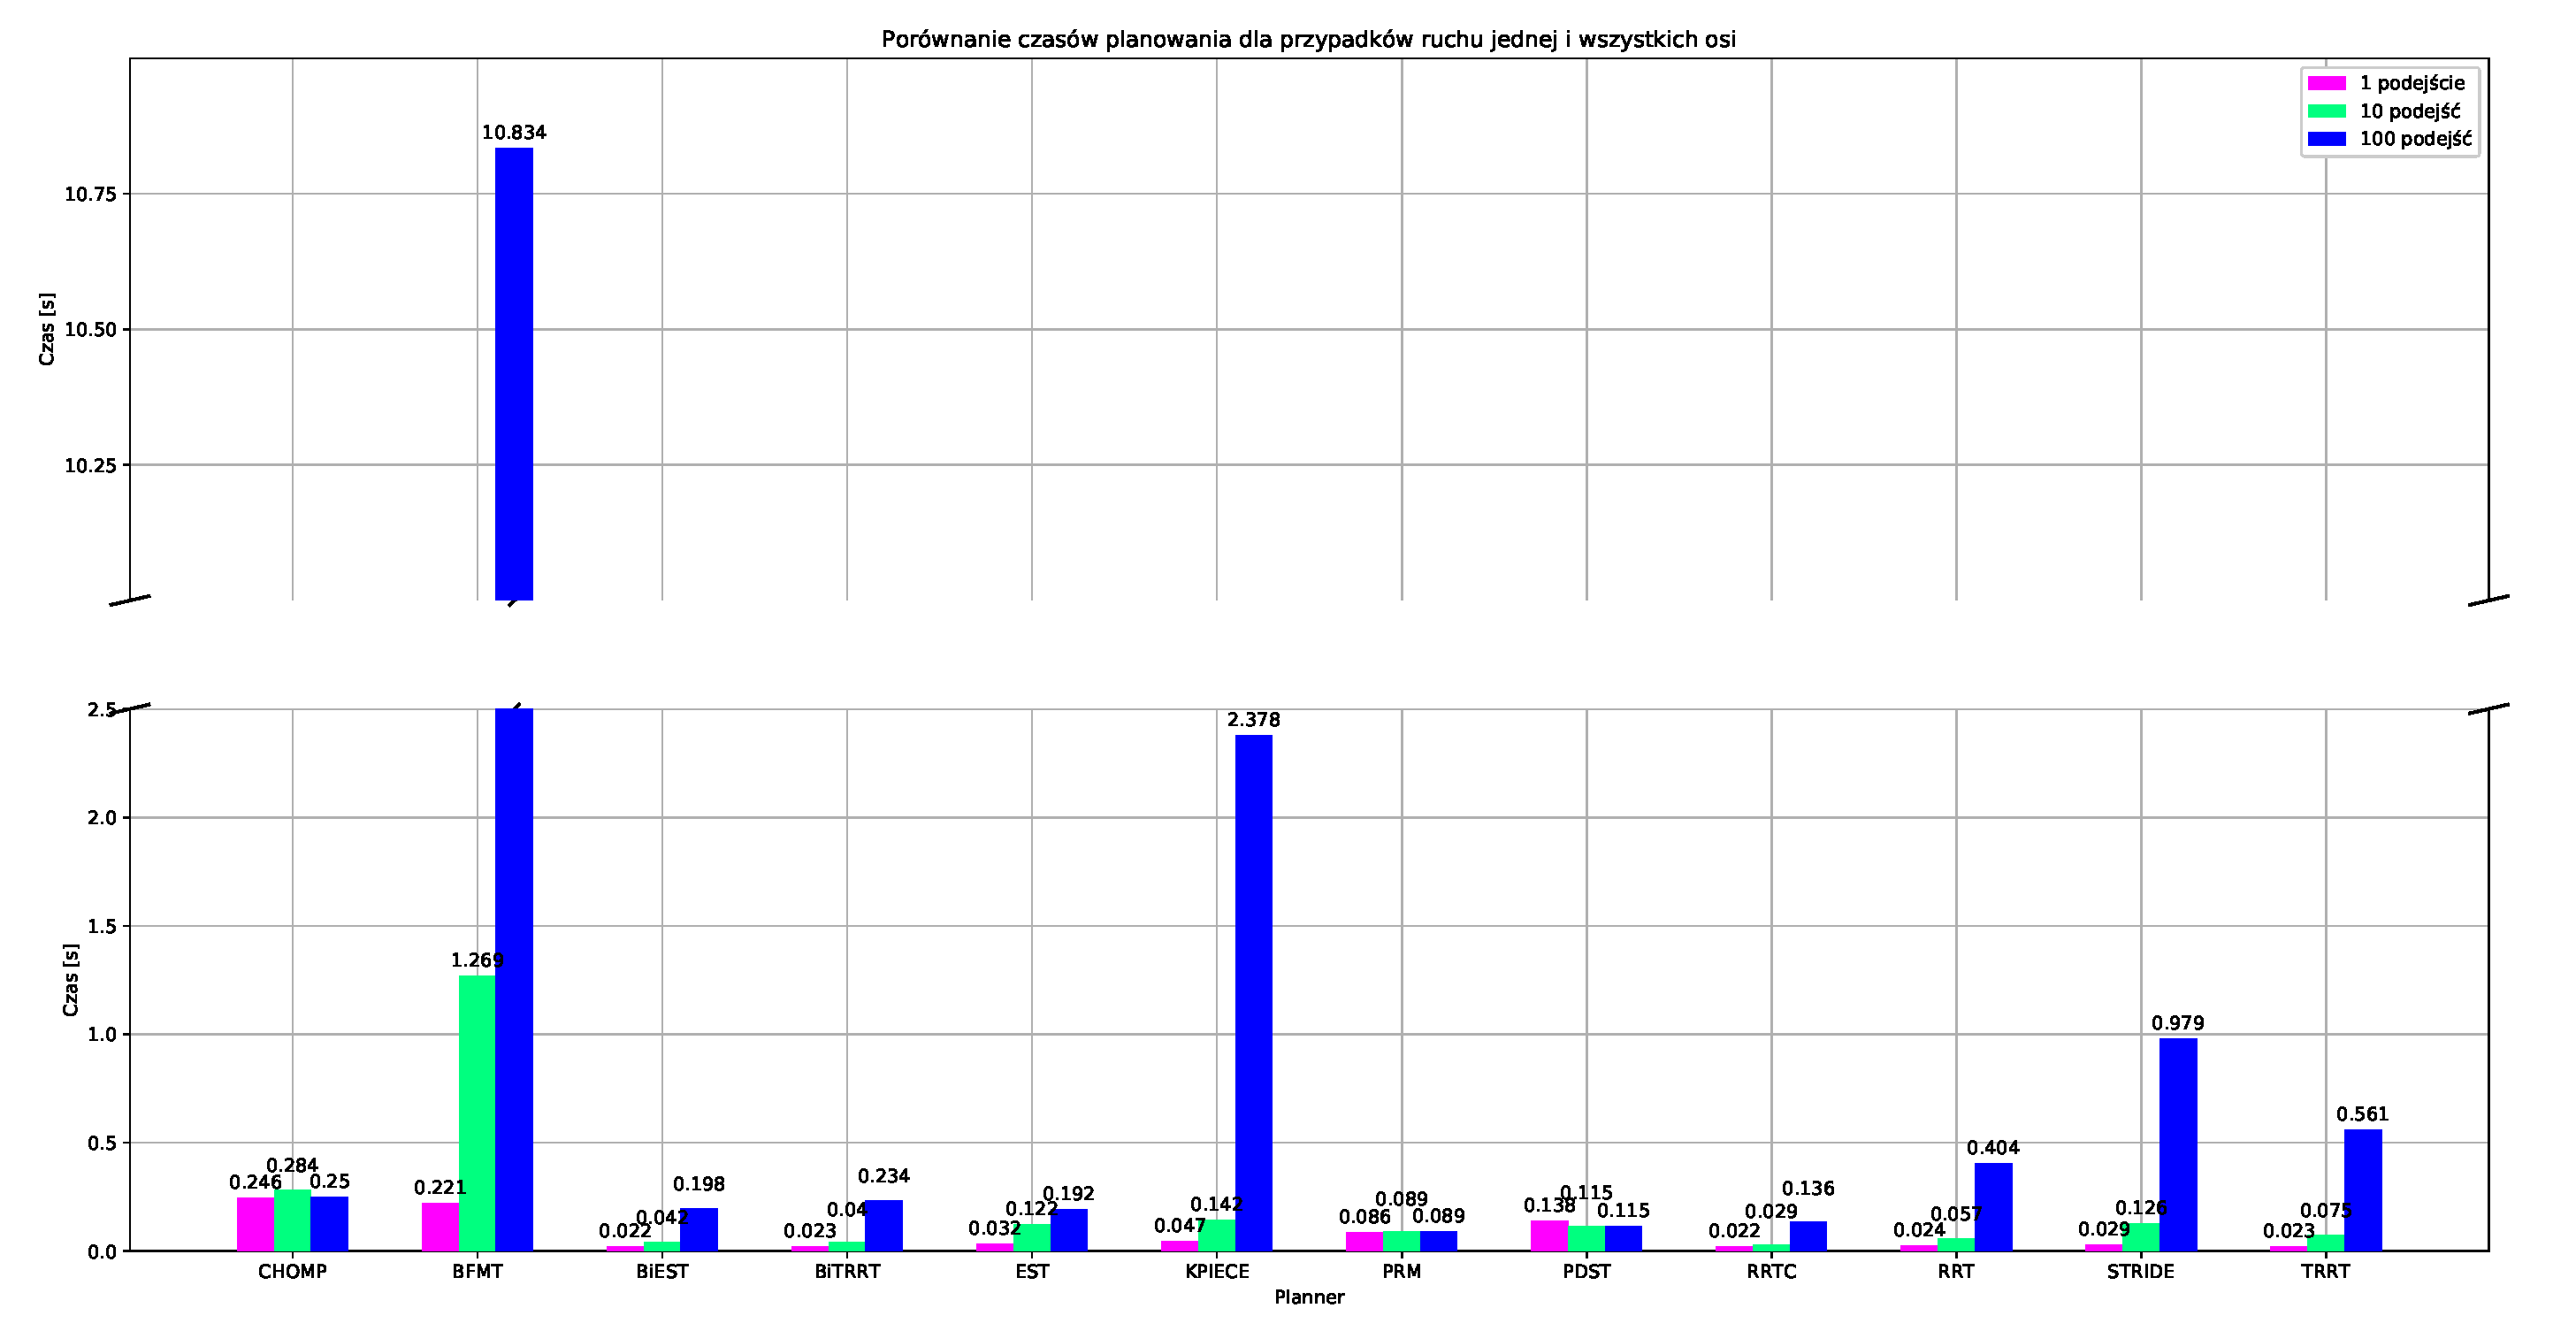
\includegraphics[width=0.9\linewidth]{{img/Figure_att_2.eps}}
	\caption{Porównanie czasów planowania dla różnej dozwolonej maksymalnej ilości prób.}
	\label{fig:31}
\end{figure}

Analizując powyższy wykres można wyróżnić na nim pewne grupy plannerów. W pierwszej z grup powinny się znaleźć takie algorytmy jak CHOMP, PRM oraz PDST. Są to plannery, dla których czasy planowania nie zależą od ilości dopuszczalnych podejść do wyznaczenia trasy. Za każdym razem otrzymywane wyniki były bardzo zbliżone. Nie dało się stwierdzić jednoznacznej tendencji. Kolejną grupę stanowi pozostała większość algorytmów, które mogąc podejść kilkukrotnie do wyznaczenia trasy, czynią to. Wydaje się, iż najgorzej w zestawieniu tym wypadają BFMT oraz KPIECE gdzie czas drastycznie się wydłuża. Przy czym jest to pewnie spowodowane faktem, iż po prostu wykorzystują dostępną możliwość wielu prób i poszukują najbardziej optymalnego rozwiązania. Takie zachowanie może być pożądane w trudniejszych zastosowaniach, wymagających np. ominięcia przeszkody. W rozpatrywanym przypadku nie daje zbyt wielu korzyści.


Wyżej wspominano, iż wszystkie prowadzone do tej pory eksperymenty zostały przeprowadzone dla domyślnie wygenerowanych nastaw plannerów. Jednak chcąc przedstawić całościowy obraz sytuacji, postanowiono sprawdzić jak modyfikacja niektórych  współczynników wpływa na otrzymywane rezultaty.
Wśród wielu parametrów możliwych do modyfikowania dla poszczególnych plannerów, jednym z podstawowych jest współczynnik odpowiadający za dokładność.

 \begin{figure}[H]
	\centering
	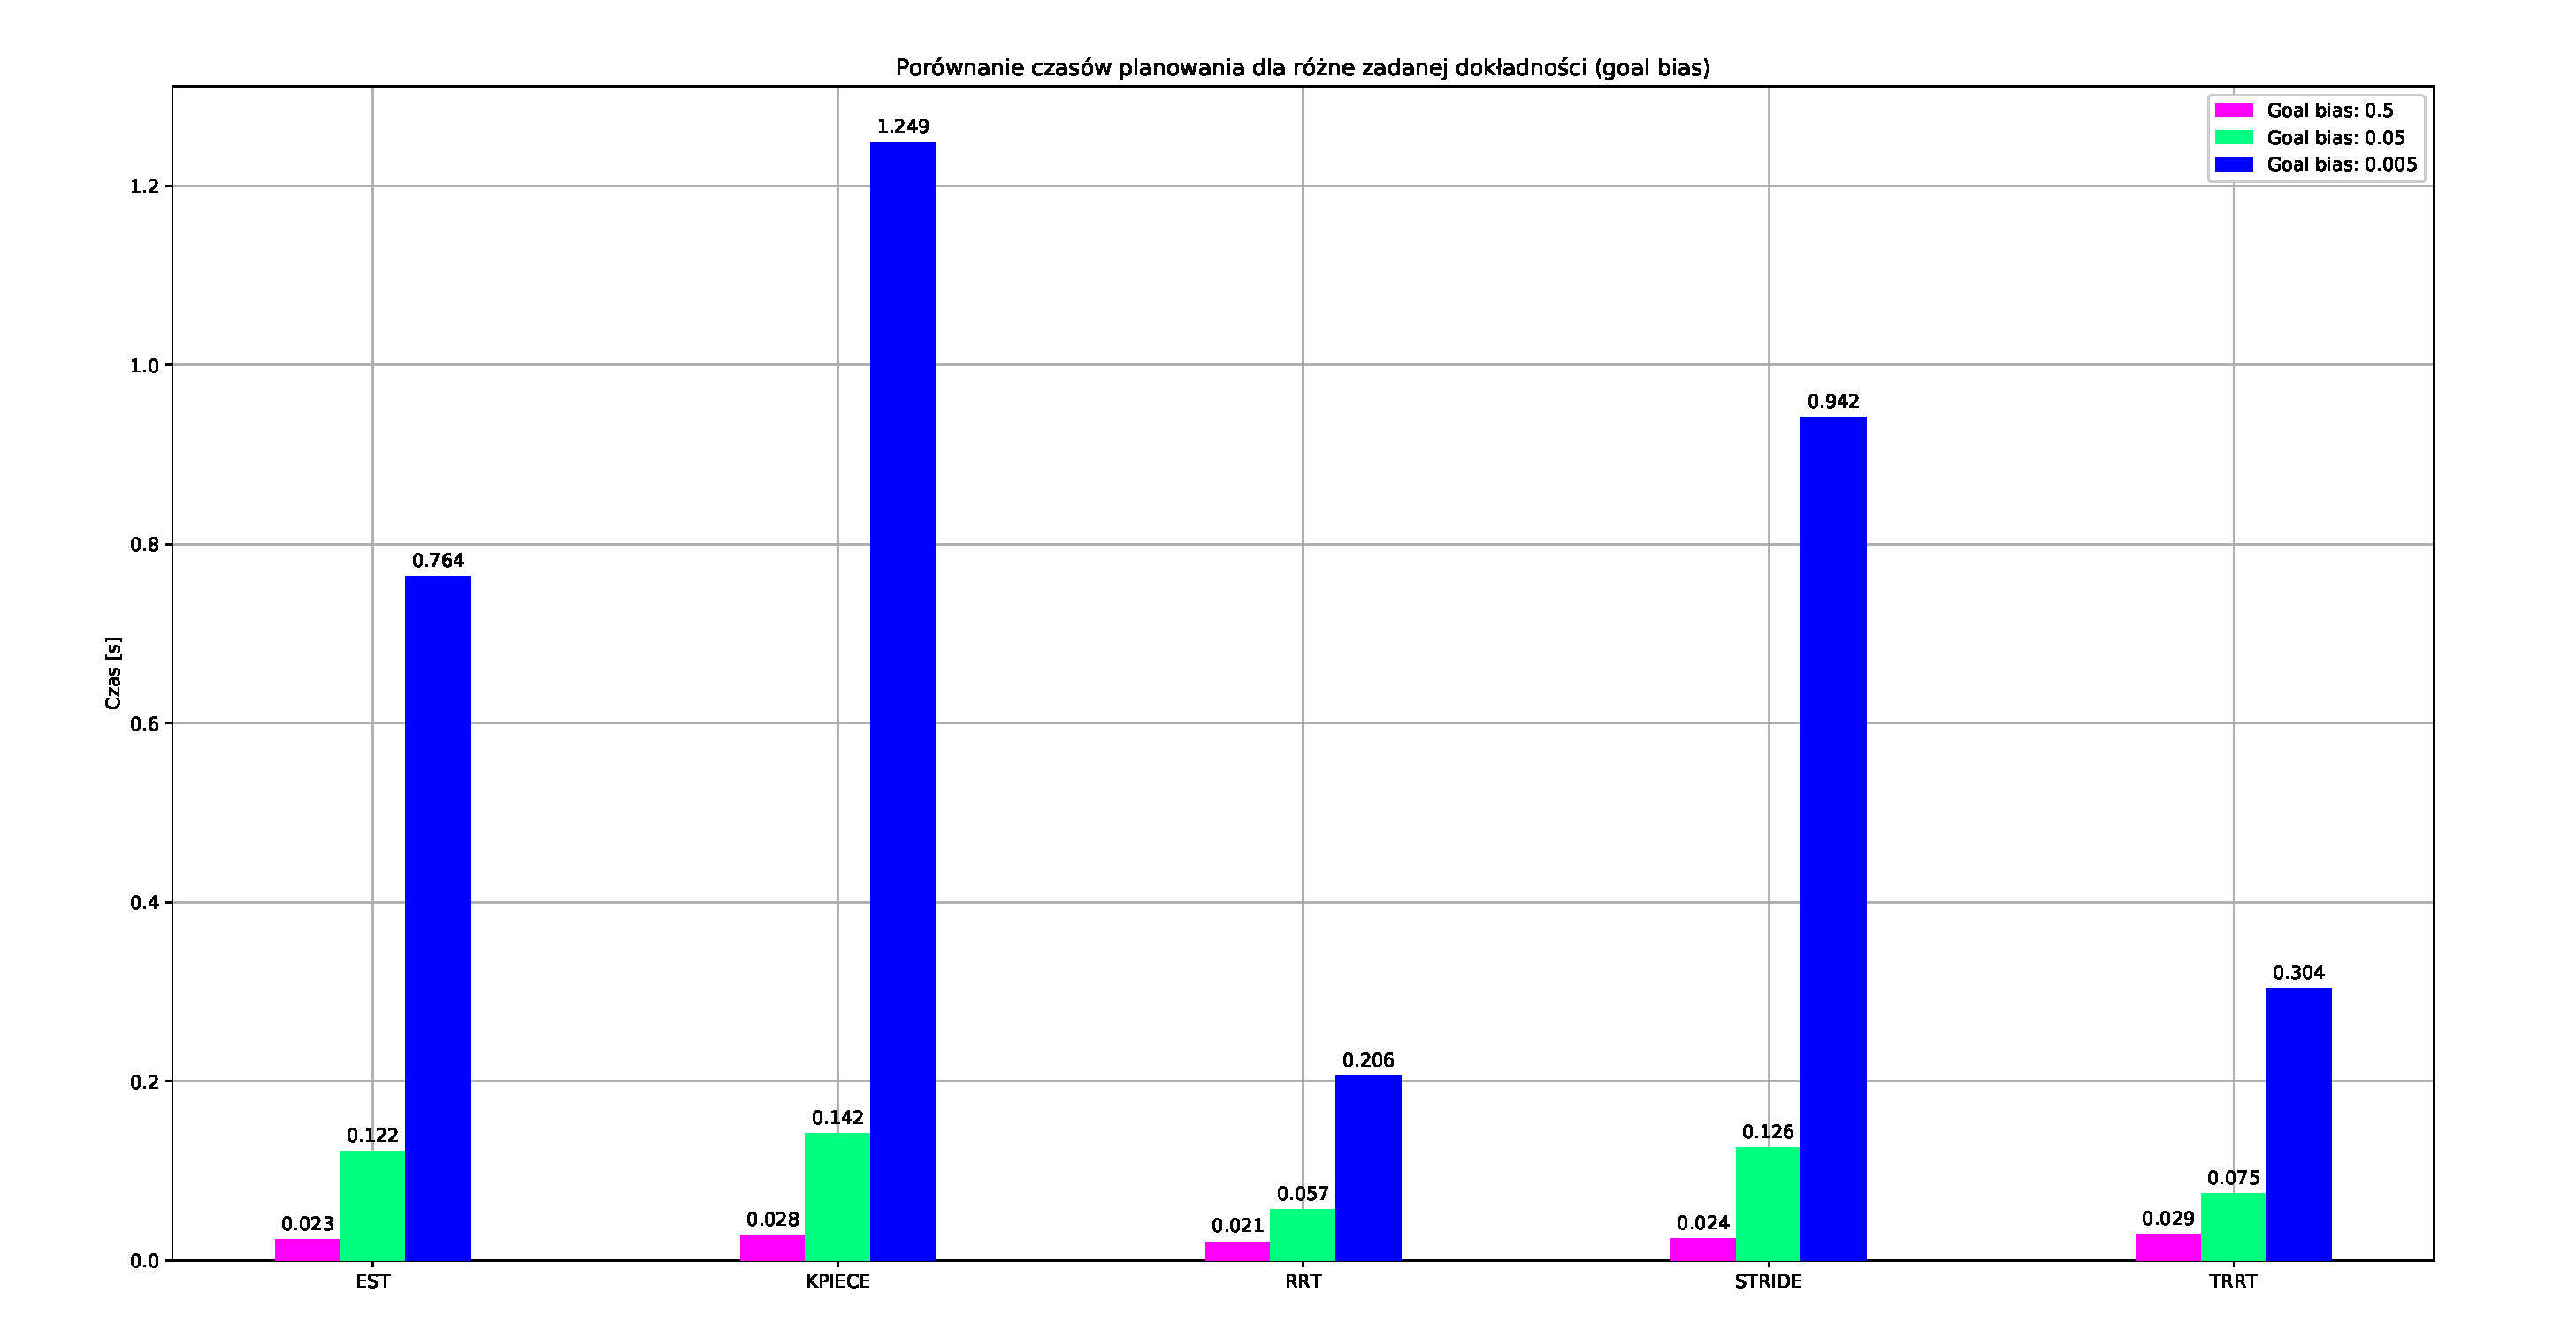
\includegraphics[width=0.9\linewidth]{{img/Figure_bias.eps}}
	\caption{Porównanie czasów planowania dla różnej zadanej dokładności (goal bias)}
	\label{fig:73}
\end{figure}

Jak można było się spodziewać - większa dokładność, wydłuża czas niezbędny na znalezienie trasy. Przy czym zależność ta jest różna dla poszczególnych plannerów. Mimo wszystko najkorzystniej wypadły dwa algorytmy - RRT oraz TRRT. Można zauważyć, iż w ich przypadkach stukrotny wzrost pożądanej dokładności, przełożył się na dziesięciokrotne wydłużenie czasu planowania (stosunek 1:10). Co jest całkiem dobrym wynikiem, zważywszy na fakt, iż dla algorytmu KPIECE zależność ta była prawie jak 1:2. 


O ile w przypadku używanego w projekcie robota precyzja zaplanowanej trasy, ze względu na mechaniczne luzy złącz, jest kwestią drugorzędną, o tyle w przypadku profesjonalnych zastosowań może stanowić kluczowy czynnik. 

Podsumowując zaprezentowane w tej sekcji wyniki eksperymentów można powiedzieć, iż każdy z algorytmów charakteryzował się specyficznymi cechami. Wydaje się, iż w przypadku prostego  zadania jakim było zwyczajne przemieszczenie wszystkich złącz optymalne pod względem czasu planowania wydają się algorytmy Pilz Industrial, gdzie wynik był praktycznie natychmiastowy. Niemniej opisane w dalszej części rozdziału, pewne ich cechy mogą powodować ich dyskwalifikacje. Ciężko też jednoznacznie krytykowanie którykolwiek z zestawionych algorytmów, gdyż czas planowania jest tylko jednym z nielicznych parametrów plannera.



\newpage
\subsection{Sposób poruszania}
W kolejnym teście postanowiono zbadać w jaki sposób poszczególne plannery realizują trasę. Dlatego też na kolejnym wykresie porównano prędkości złącza w kolejnych chwilach trasy, tak by sprawdzić jak realizowane jest przemieszczenie. Przetestowano ruch ramienia drugiego, przemieszczenie od 0$^\circ$ do -30$^\circ$. Nastawy plannerów były domyślne.

 \begin{figure}[H]
	\centering
	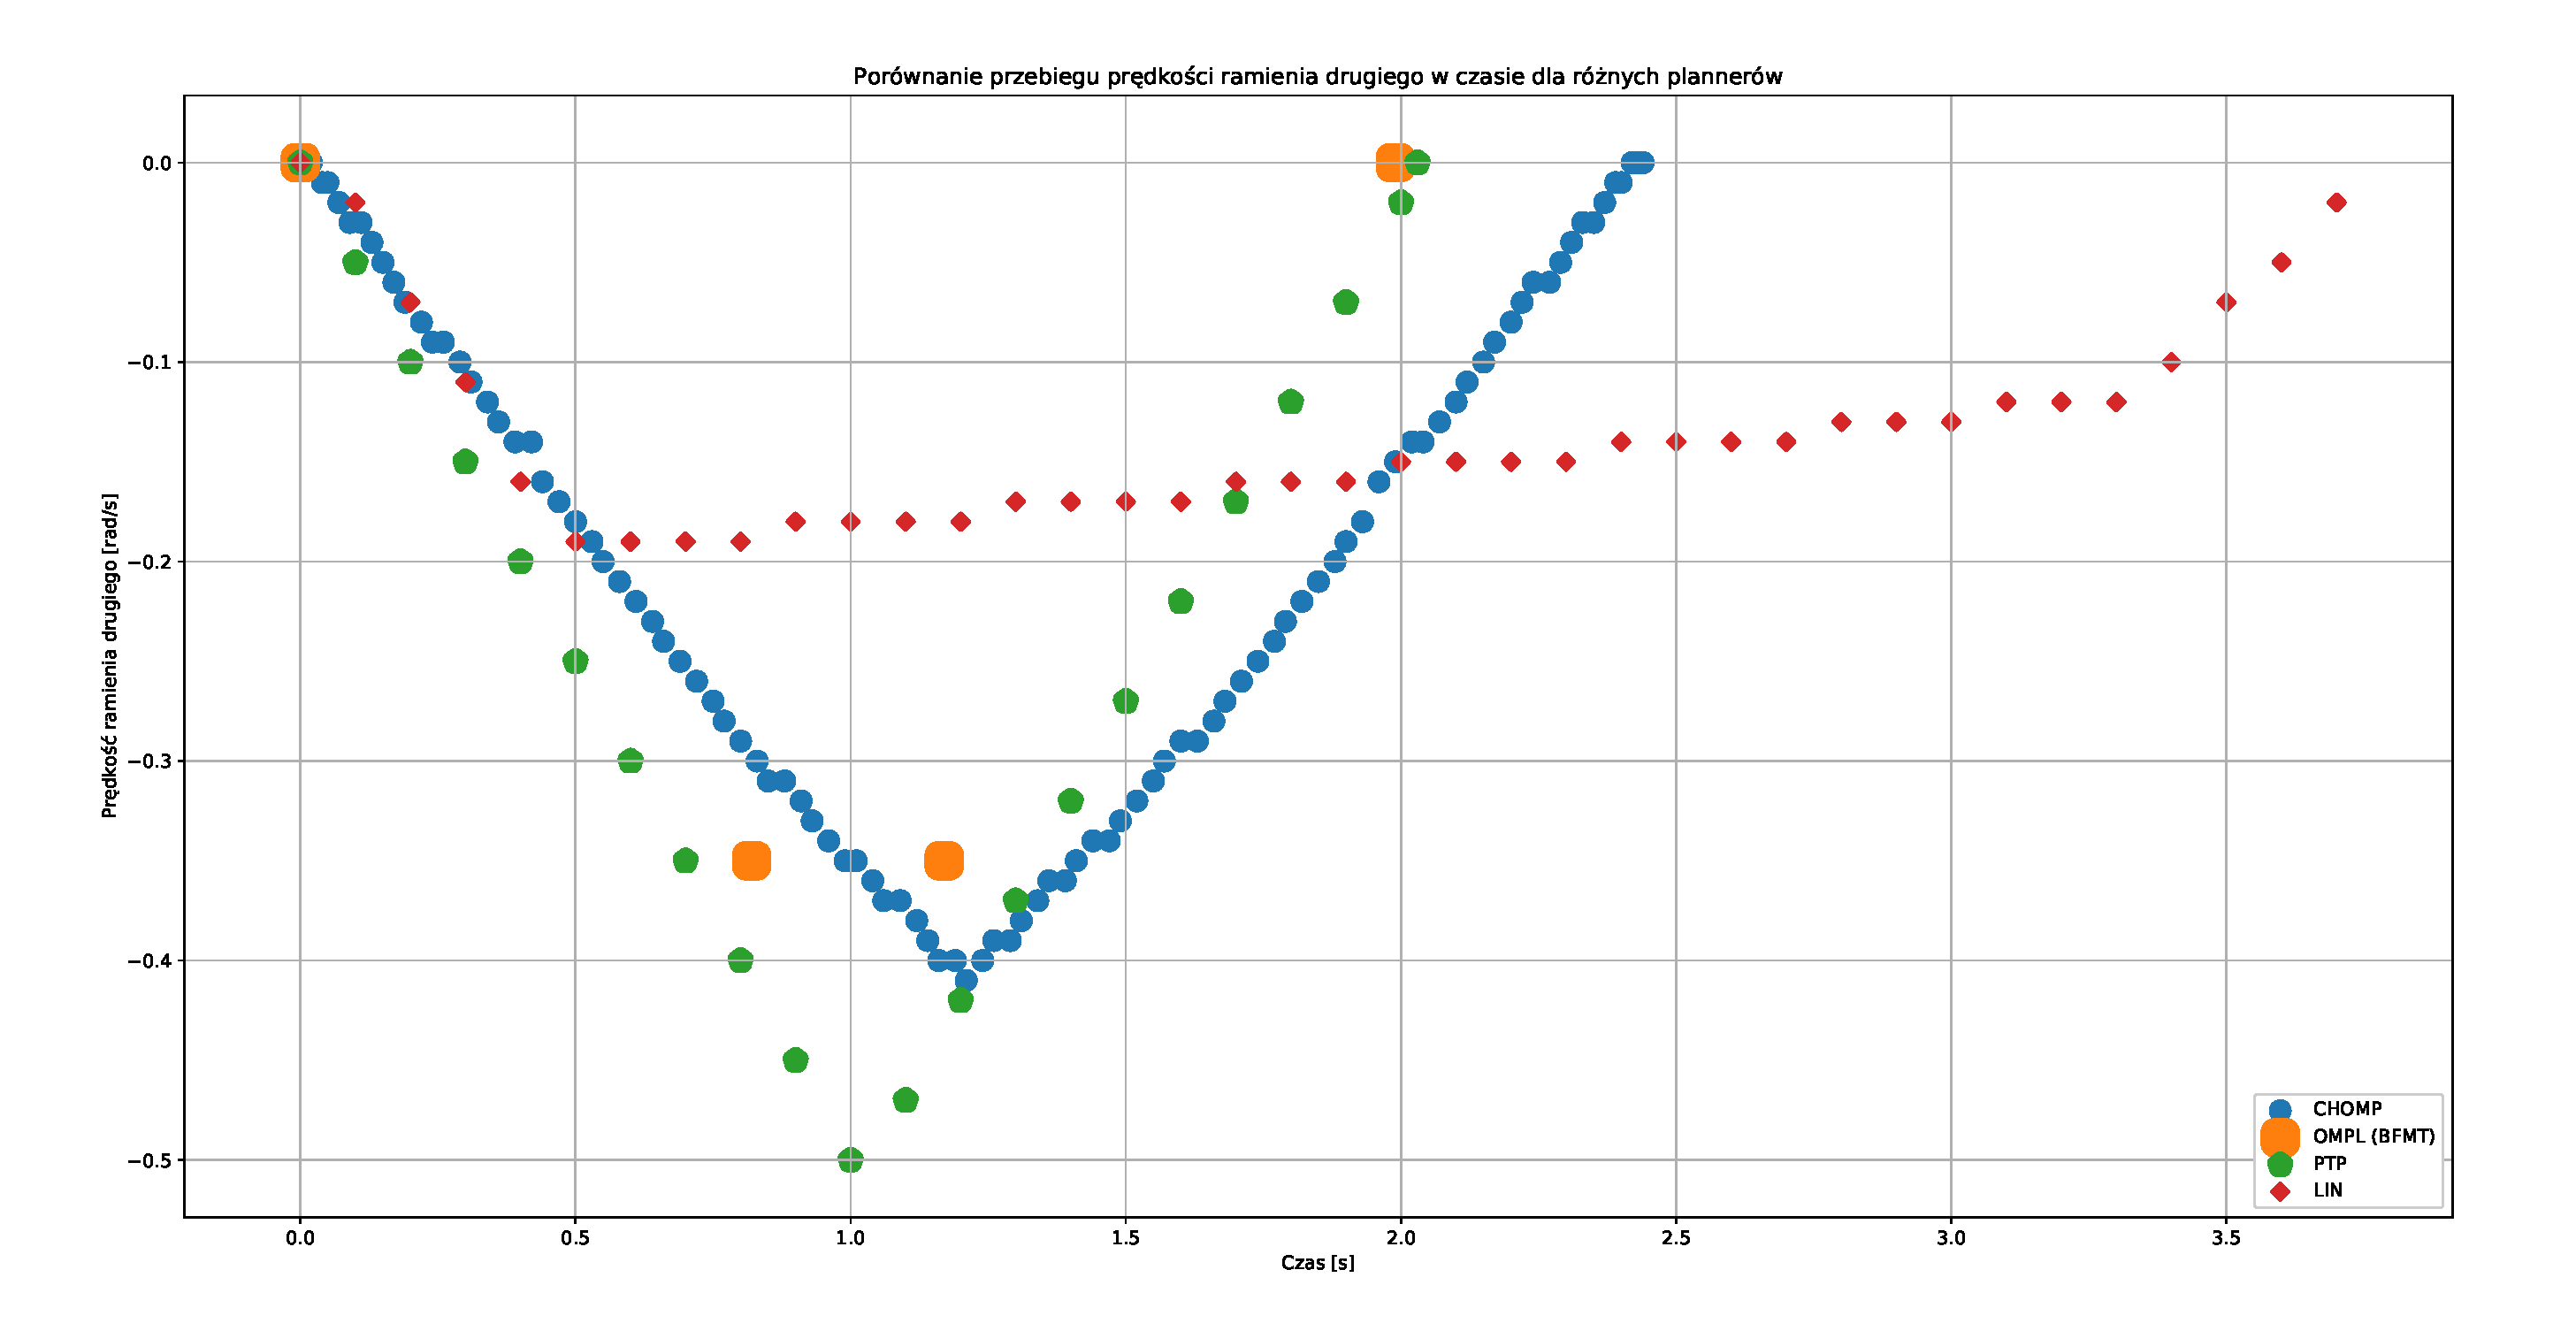
\includegraphics[width=1\linewidth]{{img/Figure_vel.eps}}
	\caption{Porównanie prędkości złącza ramienia drugiego w zależności od użytego plannera. \cite{plot_file}}
	\label{fig:10}
\end{figure}

Na powyższym wykresie można dostrzec prędkości odpowiadające punktom zaplanowanym przez poszczególne algorytmy. Wszystkie plannery wchodzące w skład grupy OMPL zachowywały się identycznie toteż nie prezentowano ich z osobna. Można zauważyć, iż CHOMP charakteryzuje się bardzo gęstym planowaniem kolejnych punktów. Przez to może zapewniać najdokładniejsze prowadzenie. Najszybsze przemieszczenie wydają się realizaować plannery OMPL oraz PTP. Ciekawy jest również kształt wszystkich przebiegów. Zarówno PTP jak i CHOMP dzielą trasę na dwie części.  W pierwszym fragmencie złącza przyśpieszają, w kolejnym hamują. Nieco inaczej trasę realizują algorytmy grupy OMPL, gdzie przebieg prędkości przypomina kształtem trapez. Trajektoria wygenerowana przez planner LIN mimo, iż najdłuższa to wydaje się być dokładna, ze względu na ilość punktów. Posiada też charakterystyczny kształt.  

W kolejnym kroku postanowiono powtórzyć eksperyment, zwiększają jednak długość przemieszczenia. Chciano w ten sposób sprawdzić czy ilość generowanych punktów jest stała, czy jednak nie, a także jak plannery odnoszą się do kwestii prędkości złącz. Testy wykonano na identycznych nastawach jak poprzednio, z tą różnicą, iż przemieszczenie wynosiło 90$^\circ$ (od +5$^\circ$0 do -40$^\circ$).

 \begin{figure}[H]
	\centering
	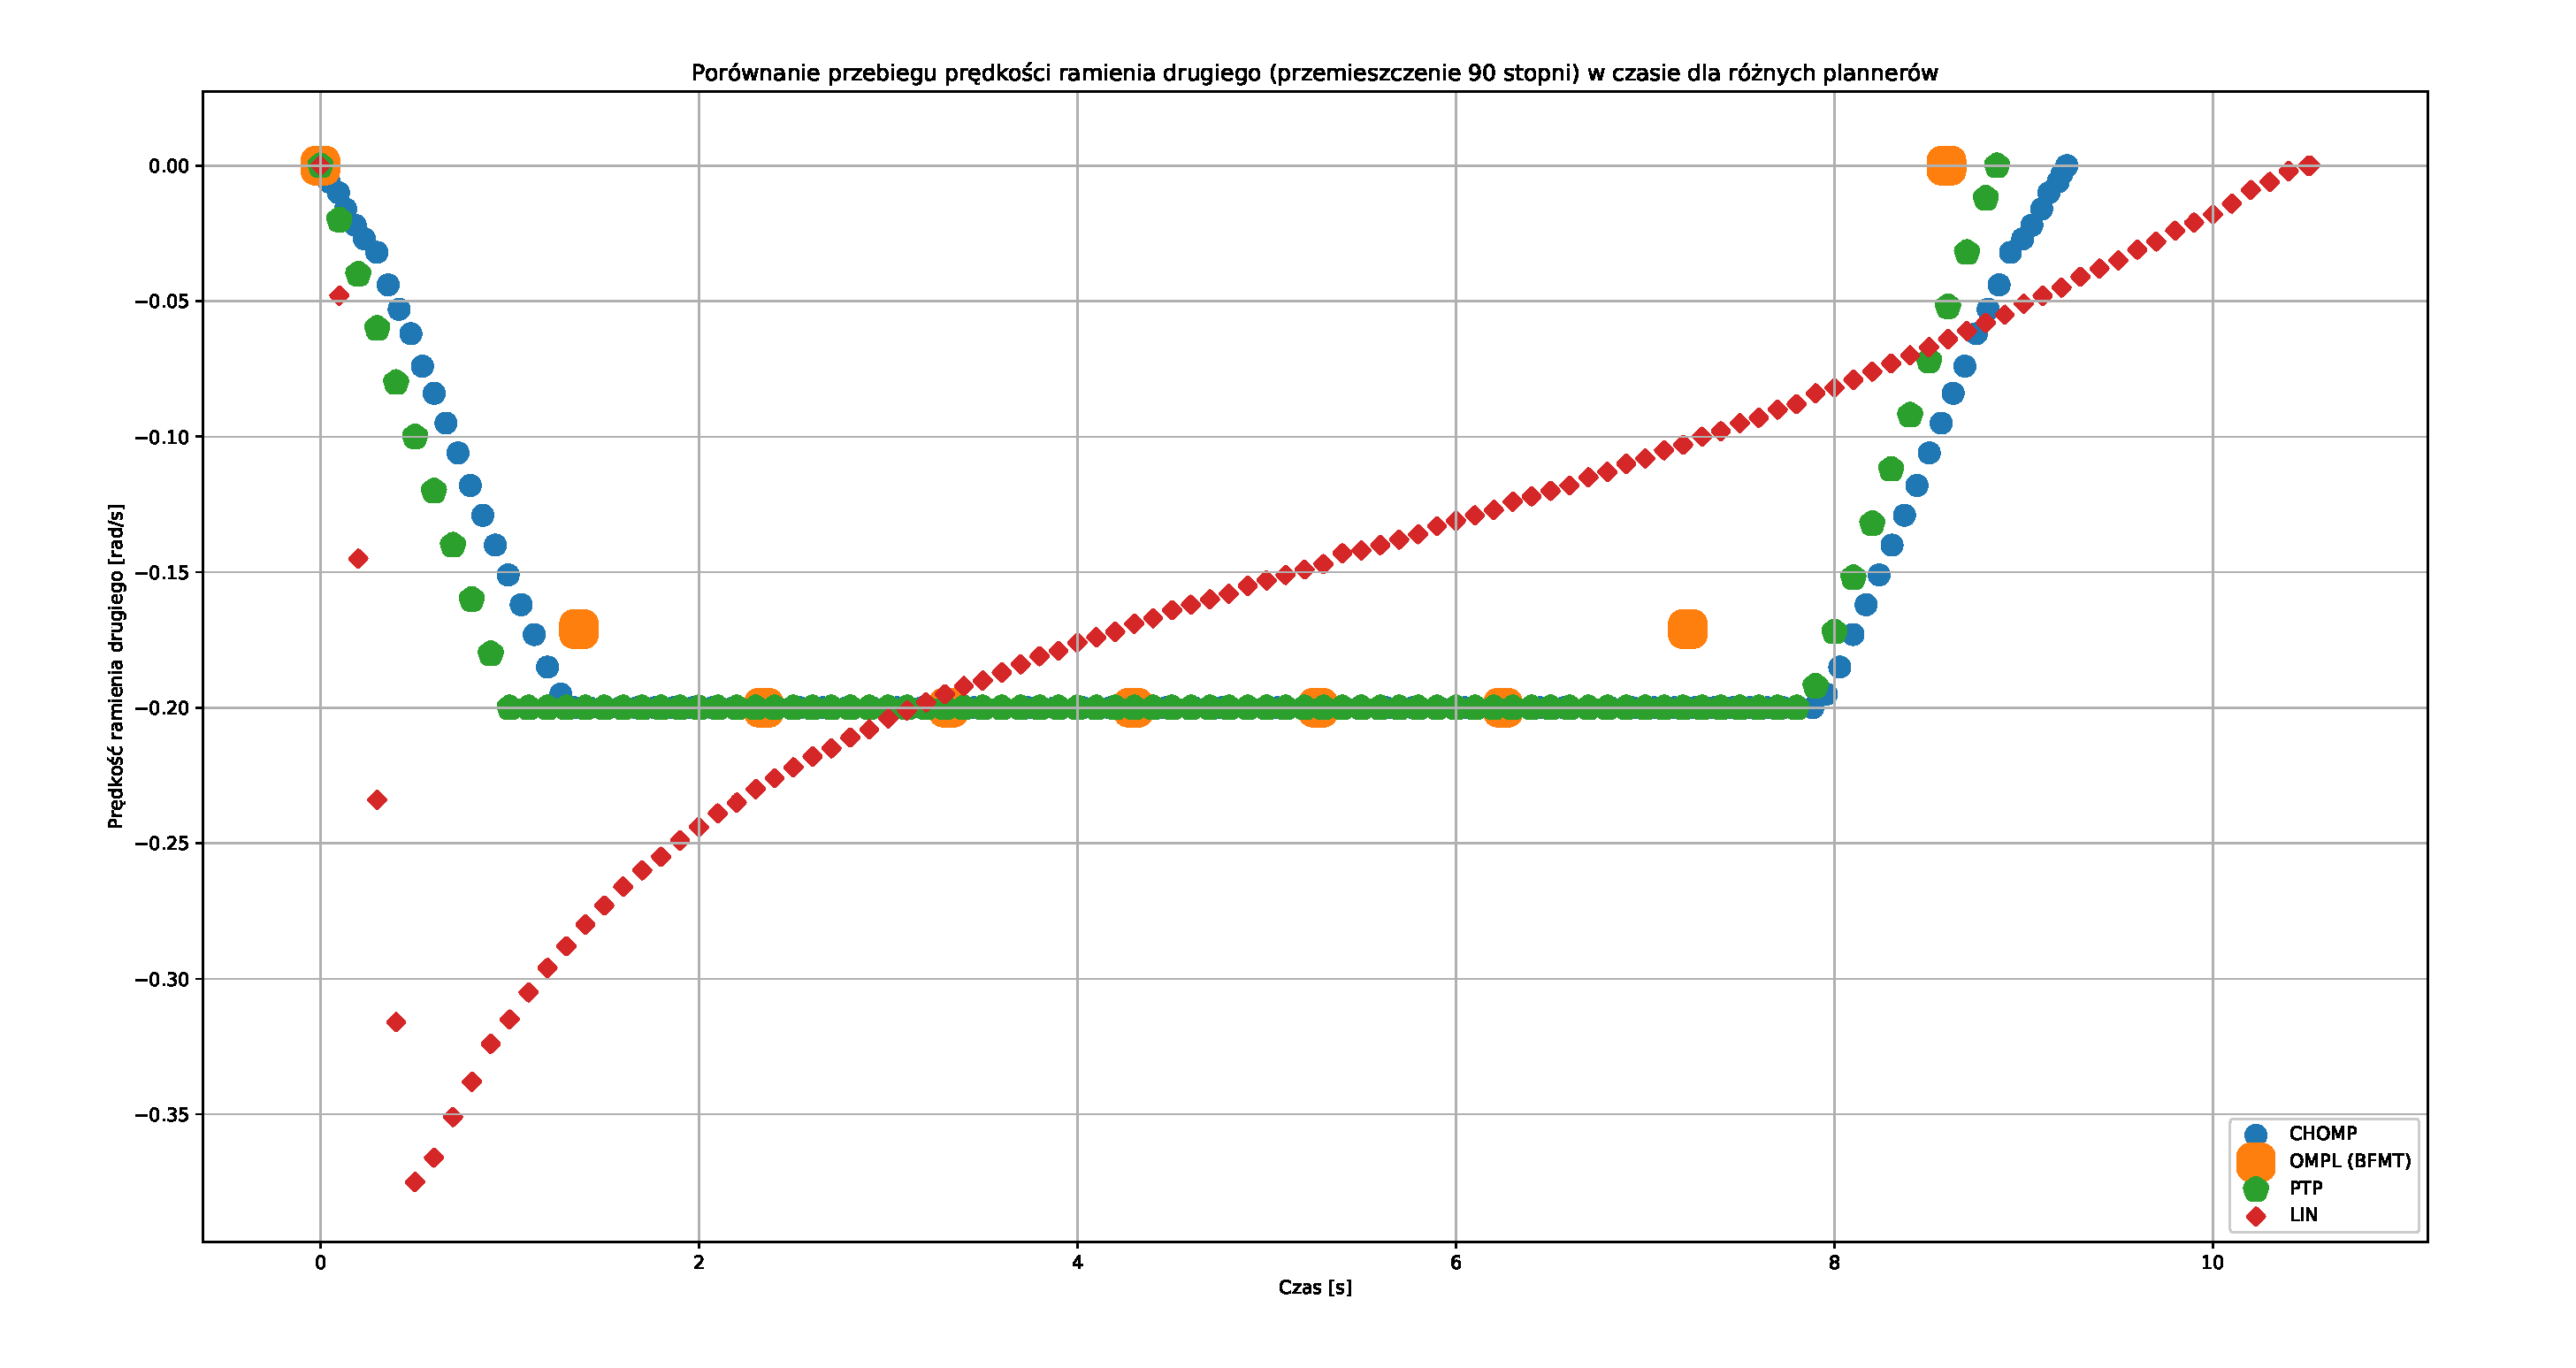
\includegraphics[width=1\linewidth]{{img/Figure_vel_90.eps}}
	\caption{Porównanie prędkości złącza ramienia drugiego w zależności od użytego plannera. \cite{plot_file}}
	\label{fig:32}
\end{figure}

Powyższy wykres \ref{fig:32} jednoznacznie odpowiada na poruszone w poprzednim akapicie kwestie. Mianowicie ilość generowanych przez plannery punktów nie jest stała - zależy od trasy. Wykres \ref{fig:32} uwypukla także charakterystyczny kształt realizacji trasy przez algorytm LIN.

Postanowiono także sprawdzić czy punkty generowane są w równych odstępach czasu, czy jednak nie. W tym celu wyznaczono minimalne i maksymalne różnice czasów między kolejnymi próbkami poprzedniego wykresu.

% Please add the following required packages to your document preamble:
% \usepackage{multirow}
% \usepackage[table,xcdraw]{xcolor}
% If you use beamer only pass "xcolor=table" option, i.e. \documentclass[xcolor=table]{beamer}
\begin{table}[H]
\centering
\caption{Porównanie różnic czasu między kolejnymi próbkami plannerów}
\label{tab:18}
\begin{tabular}{|c|c|c|c|
>{\columncolor[HTML]{C0C0C0}}c |ll}
\cline{1-5}
\cellcolor[HTML]{C0C0C0}L.p. & \cellcolor[HTML]{C0C0C0}{\color[HTML]{000000} \begin{tabular}[c]{@{}c@{}}Grupa \\ plannerów\end{tabular}} & \cellcolor[HTML]{C0C0C0}Planner & \cellcolor[HTML]{C0C0C0}\begin{tabular}[c]{@{}c@{}}Min. różnica czasu\\ między próbkami {[}s{]}\end{tabular} & \begin{tabular}[c]{@{}c@{}}Max. różnica czasu\\ między próbkami {[}s{]}\end{tabular} &  &  \\ \cline{1-5}
\cellcolor[HTML]{EFEFEF}1.   & CHOMP                                                                                                     & \cellcolor[HTML]{EFEFEF}CHOMP   & \cellcolor[HTML]{EFEFEF}0.01(9)                                                                              & \cellcolor[HTML]{EFEFEF}0.147                                                        &  &  \\ \cline{1-5}
\cellcolor[HTML]{C0C0C0}2.   & OMPL                                                                                                      & \cellcolor[HTML]{C0C0C0}BFMT    & \cellcolor[HTML]{C0C0C0}0.976                                                                                & 1.366                                                                                &  &  \\ \cline{1-5}
\cellcolor[HTML]{EFEFEF}3.   &                                                                                                           & \cellcolor[HTML]{EFEFEF}PTP     & \cellcolor[HTML]{EFEFEF}0.0(9)                                                                               & \cellcolor[HTML]{EFEFEF}0.1                                                          &  &  \\ \cline{1-1} \cline{3-5}
\cellcolor[HTML]{C0C0C0}4.   & \multirow{-2}{*}{\begin{tabular}[c]{@{}c@{}}Pilz Industrial \\ Motion Planner\end{tabular}}               & \cellcolor[HTML]{C0C0C0}LIN     & \cellcolor[HTML]{C0C0C0}0.0(9)                                                                               & 0.1                                                                                  &  &  \\ \cline{1-5}
\end{tabular}
\end{table}

Tabela obrazuje, iż największą zmienność w generowaniu próbek posiada algorytm CHOMP. Daje to istotną informację, że wraz ze zbliżaniem się do kluczowych elementów trasy, próbki zagęszczają się. Zmienność występuje także w przypadku grupy OMPL. Plannery Pilz Industrial raczej zdają się utrzymywać stały krok wyznaczania kolejnych punktów.

Dodatkowo według przeprowadzonych testów, ilość punktów jakie generują plannery (na podstawie OMPL FMT) nie zależy od ustawionej dokładności - goal bias. Za każdym razem zarówno prędkości jak i czasy przemieszczeń były identyczne. 

%Starając się wyczerpać tematykę zaplanowanych punktów i prędkości złącz postanowiono jeszcze zestawić przebiegi wszystkich złącz, niemniej w sytuacji omijania przeszkody. Tematyka ta zostanie dokładnie omówiona w kolejnych sekcjach, niemniej celem niniejszego eksperymentu było sprawdzenie, jak zachowuje się algorytm w przypadku ruchu złożonego. Poniżej zaprezentowano wykres przedstawiający prędkości wszystkich osi - wykres \ref{fig:33}.

\begin{figure}[H]
	\centering
	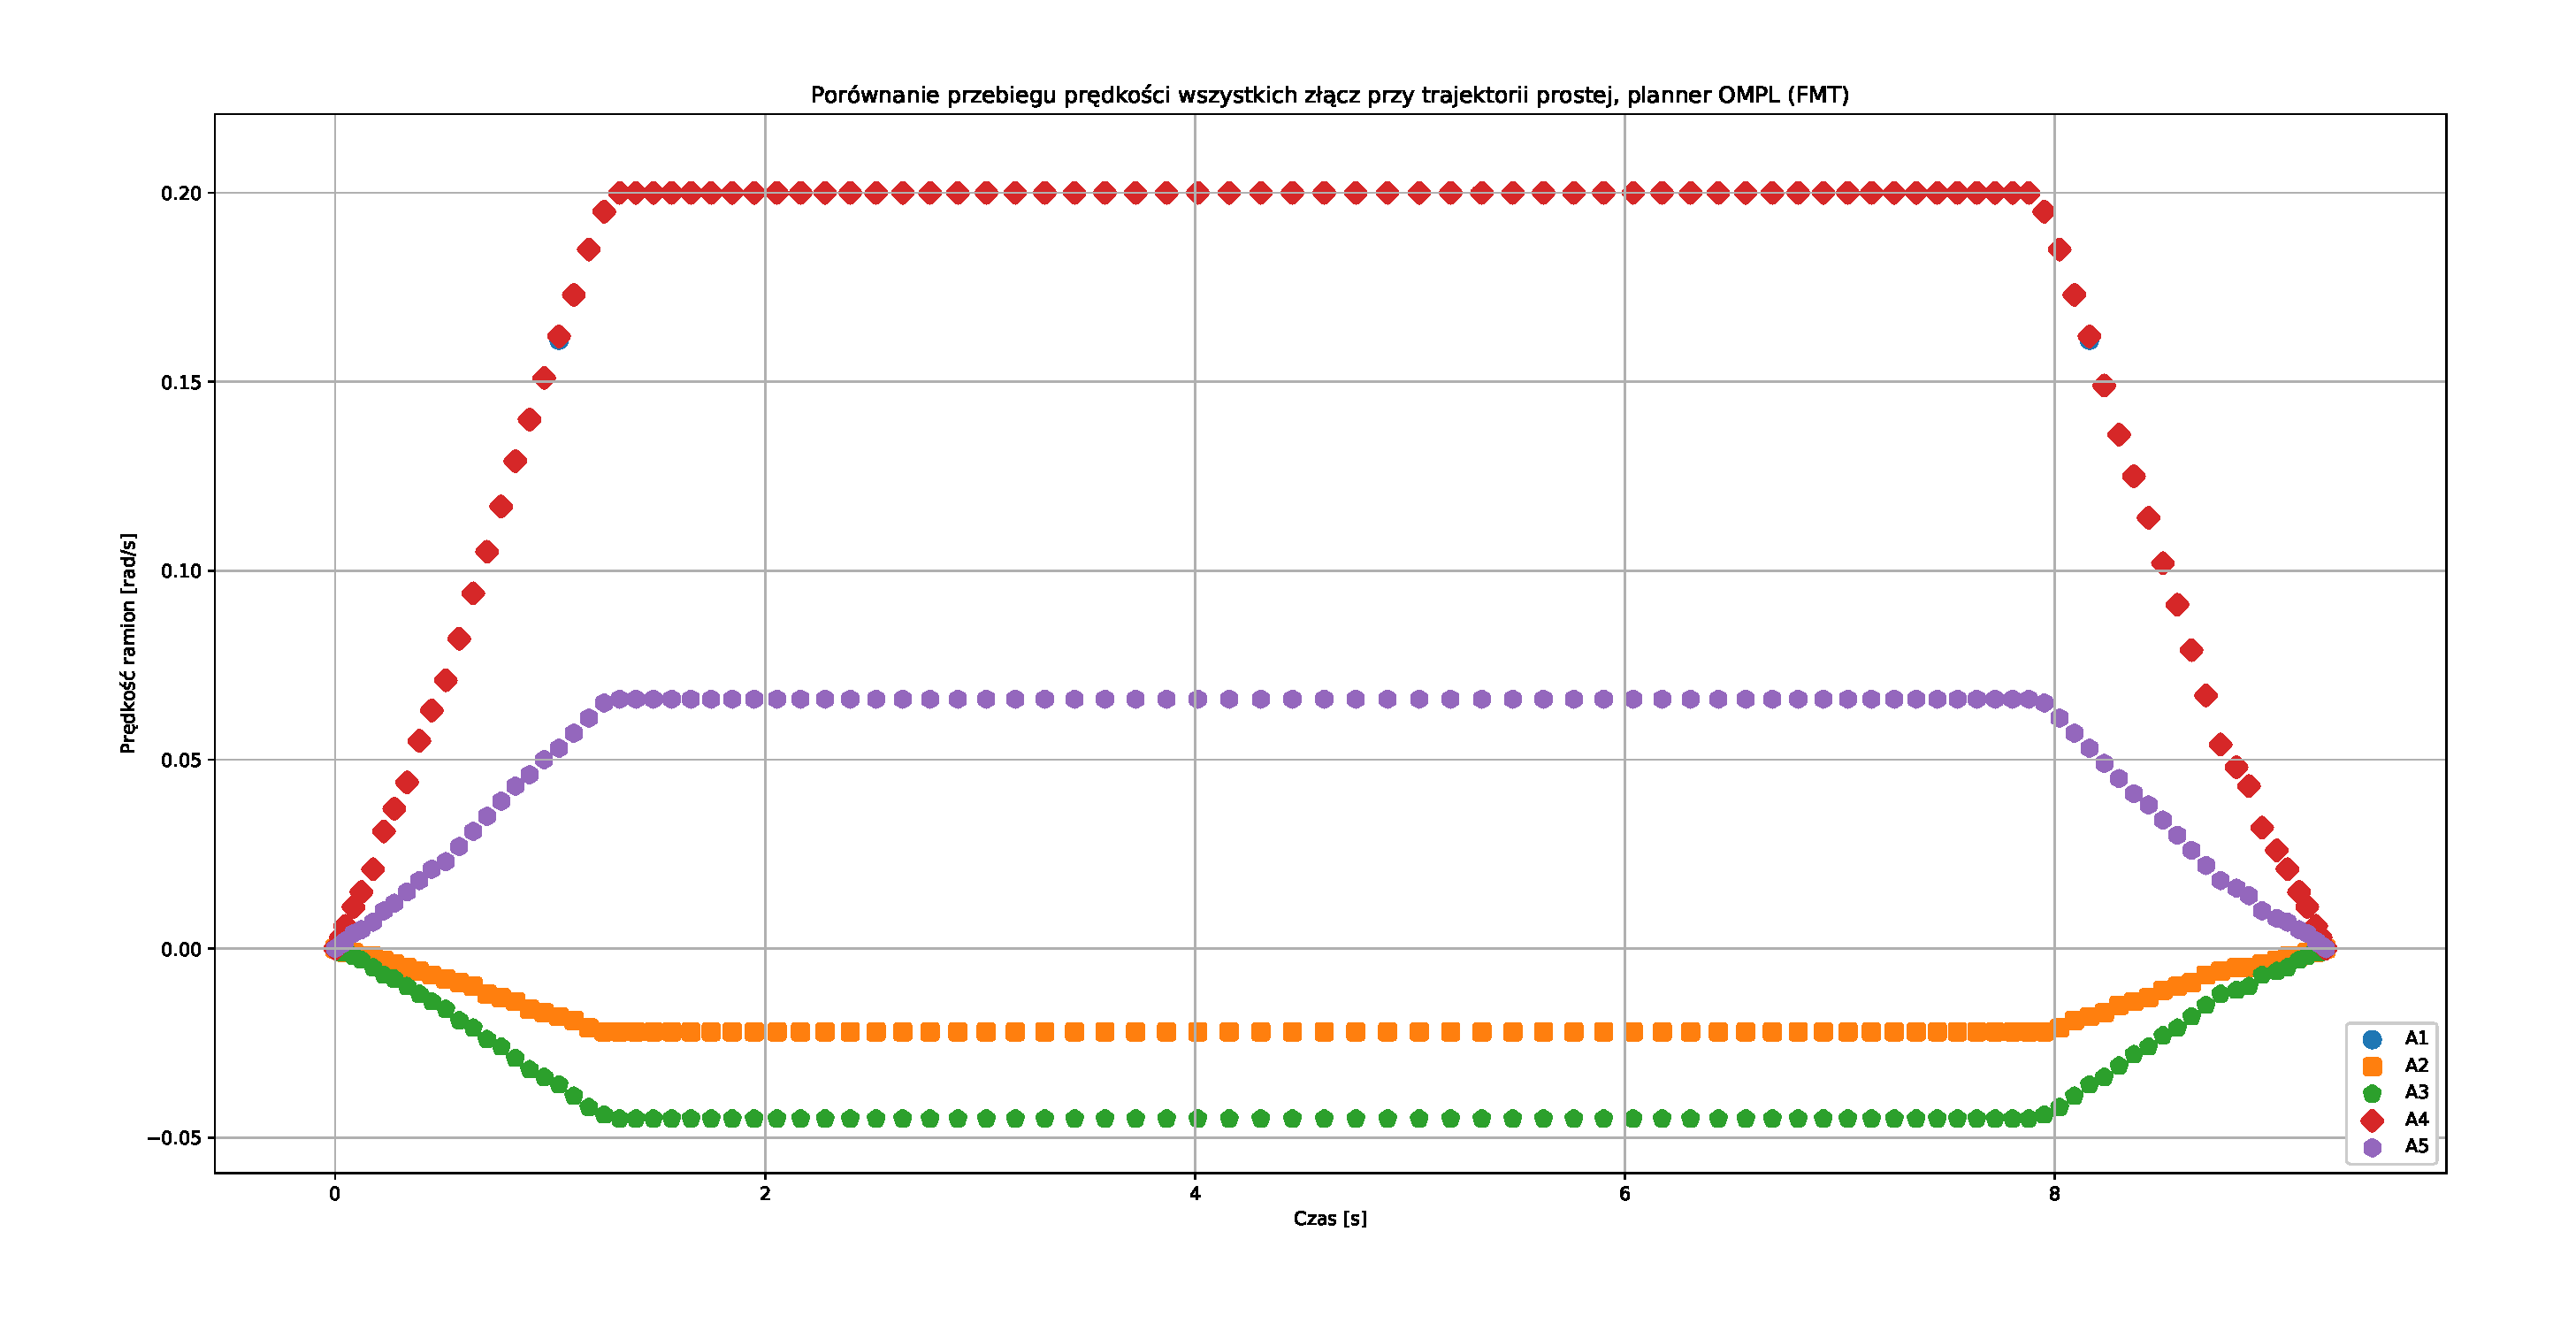
\includegraphics[width=1\linewidth]{{img/Figure_synchro.eps}}
	\caption{Porównanie prędkości wszystkich złącz przy omijaniu przeszkody dla plannera OMPL FMT. \cite{plot_file}}
	\label{fig:33}
\end{figure}


Powyższy wykres ilustruje dwie kwestie. Pierwszą rzeczą jest skalowanie prędkości złącz. Osie są względem siebie synchronizowane, tak by wszystkie zakończyły swój ruch dokładnie w tym samym czasie. Co ciekawe skalowanie prędkości poszczególnych złącz następuje w przypadku wszystkich plannerów. Nie ma tutaj także znaczenia czy następuje omijanie przeszkody, czy normalne przemieszczenie.

Druga kwestia jaką prezentuje wykres \ref{fig:33} to zagęszczanie próbek, o którym poprzednio wspominano. Na wykresie widać to doskonale.


 \newpage
 
\subsection{Omijanie przeszkód}

Niniejszy podrozdział poświęcono kwestii omijania przeszkód. Przetestowano zatem czy dany algorytm jest w stanie realizować takie zadanie, a także w jaki sposób to czyni. 

Rviz umożliwia użytkownikowi dodanie do scenografii otaczającej robota dodatkowych obiektów, które manipulator może traktować jako przedmioty kolizyjne. W tym celu zaproponowano zatem prostą sytuację, w której to robota ma przemieścić swoje ramię w płaszczyźnie pionowej, z tym zastrzeżeniem iż na trasie tej umieszczono obiekt. Całość prezentowała się tak jak poniżej - rysunek \ref{fig:34}. 

Przygotowana sytuacja była dosyć prosta, niemniej wymagała od plannera ominięcia dołączonego prostopadłościanu.  Poniższa tabela prezentuje zestawienie algorytmów ze względu na te które potrafiły i nie potrafiły znaleźć trasy.

\begin{figure}[H]
	\centering
	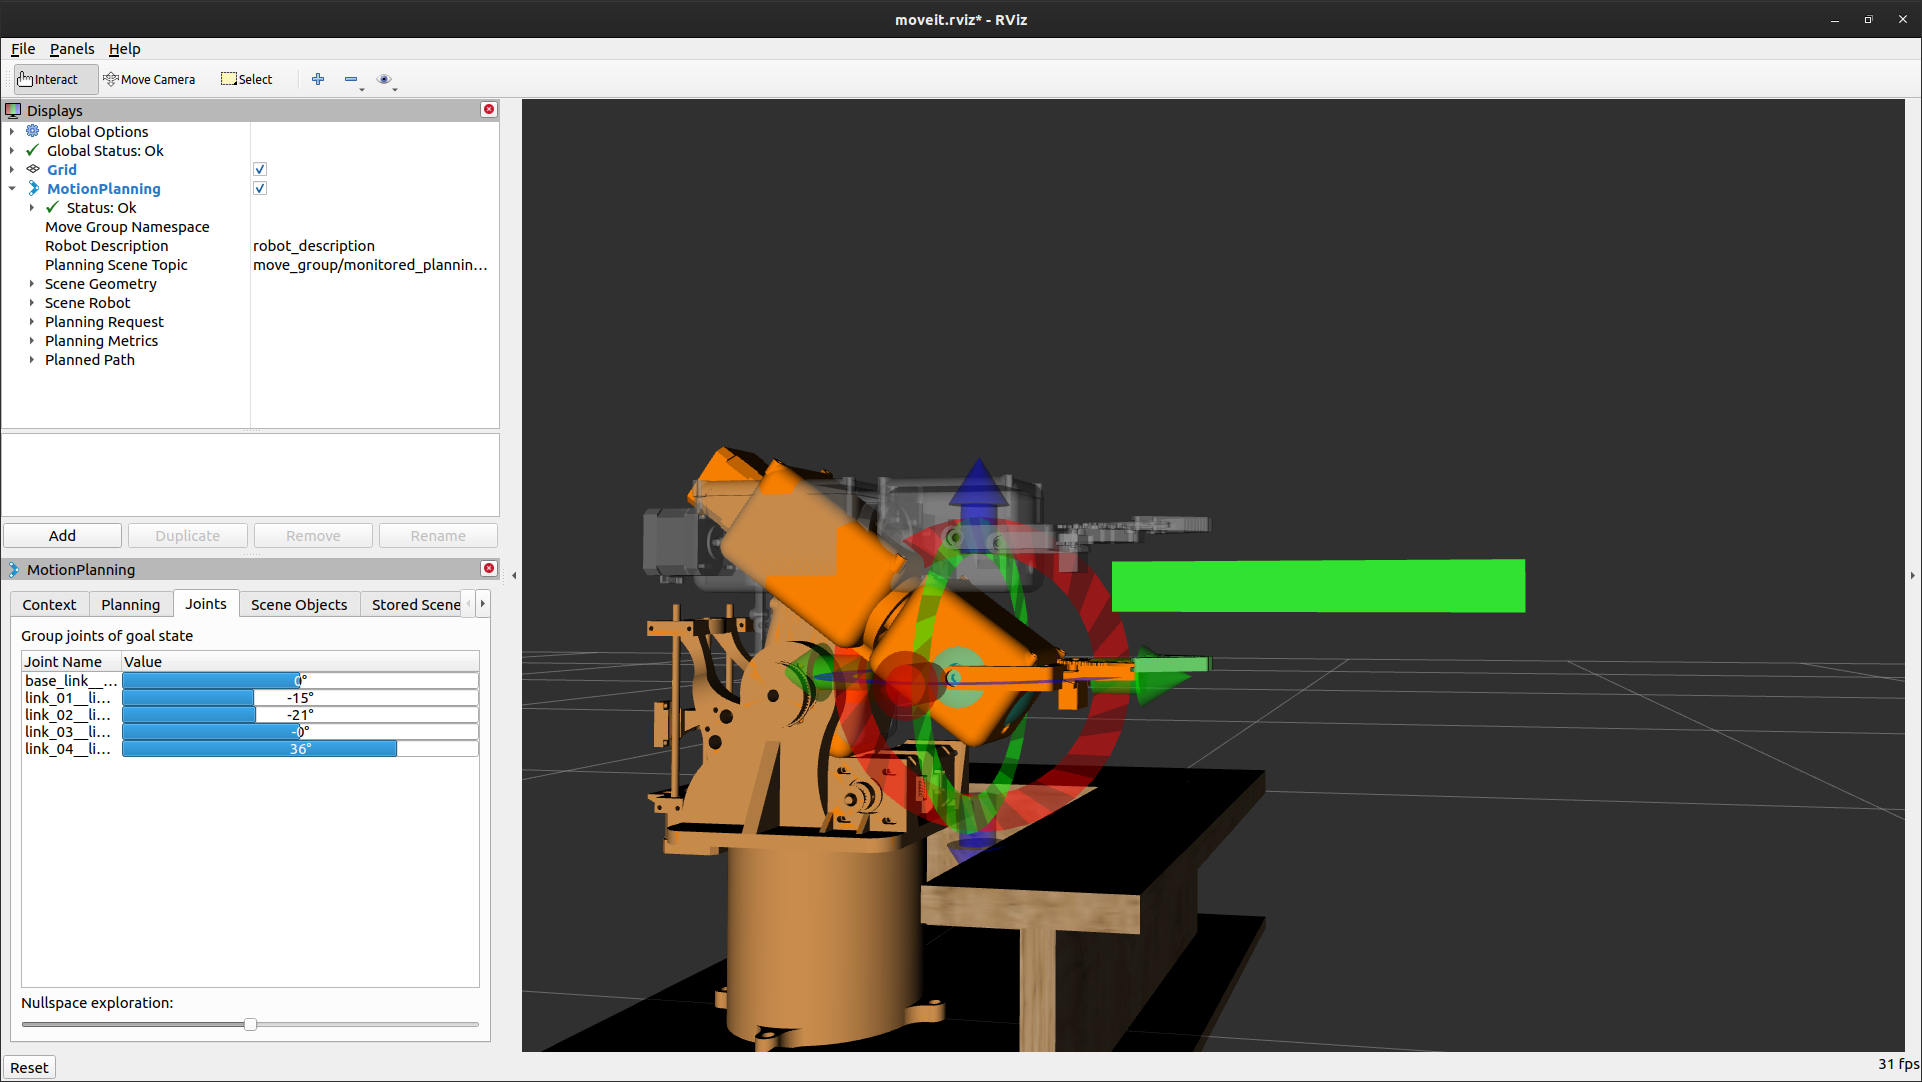
\includegraphics[width=1\linewidth]{{img/Bild_rviz_scene.png}}
	\caption{\centering Przygotowany scenariusz omijania przeszkody w programie Rviz. \cite{own}, \cite{oak}}
	\label{fig:34}
\end{figure}


W czasie eksperymentów wyszło, iż zarówno plannery grupy CHOMP oraz Pilz Industrial nie są w stanie omijać przeszkód. Jest to bardzo istotne przy ewentualnej chęci ich stosowania. Zatem eksperymenty przeprowadzano jedynie na grupie algorytmów OMPL. W poniższej tabeli zestawiono otrzymane rezultaty. Przy czym te plannery, które nie zostały w niej zawarte nie były  w stanie zaplanować trasy przy narzuconych warunkach. 

Ustawienia były w każdym przypadku domyślne. Maksymalna ilość prób jaką miały do wykorzystania algorytmy ustawiono na 10, natomiast czas planowania - 10 sekund. Za każdym razem dokonywano 10 prób. Długości tras jakie zestawiono w poniższej tabeli \ref{tab:7} odnoszą się do sumarycznego przemieszczenia wszystkich złącz na całej trasie. Natomiast czasy oznaczają ustalony teoretyczny czas potrzebny na realizację trajektorii.

% Please add the following required packages to your document preamble:
% \usepackage[table,xcdraw]{xcolor}
% If you use beamer only pass "xcolor=table" option, i.e. \documentclass[xcolor=table]{beamer}
\begin{table}[H]
\centering
\caption{Zestawienie długości i czasów zaplanowanych tras przy omijaniu przeszkody}
\label{tab:7}
\begin{tabular}{|c|c|c|c|c|c|c|c|}
\hline
\rowcolor[HTML]{C0C0C0} 
Lp  & Planner  & \begin{tabular}[c]{@{}c@{}}Min. wy. \\ trasa \\ {[}rad{]}\end{tabular} & \cellcolor[HTML]{C0C0C0}\begin{tabular}[c]{@{}c@{}}Max. wy.\\  trasa \\ {[}rad{]}\end{tabular} & \begin{tabular}[c]{@{}c@{}}Śr. wy.\\ trasa 10 \\ pr. {[}rad{]}\end{tabular} & \cellcolor[HTML]{C0C0C0}\begin{tabular}[c]{@{}c@{}}Min. wy.\\ czas {[}s{]}\end{tabular} & \cellcolor[HTML]{C0C0C0}\begin{tabular}[c]{@{}c@{}}Max. wy.\\  czas {[}s{]}\end{tabular} & \cellcolor[HTML]{C0C0C0}\begin{tabular}[c]{@{}c@{}}Śr. czas \\ 10 pr. \\ {[}s{]}\end{tabular} \\ \hline
\rowcolor[HTML]{9AFF99} 
1.  & BFMT     & 7.791                                                                  & 10.262                                                                                         & 9.228                                                                       & 5.248                                                                                   & 5.965                                                                                    & 5.494                                                                                         \\ \hline
\rowcolor[HTML]{FFCCC9} 
2.  & BKPIECE  & 15.008                                                                 & 262.628                                                                                        & 158.649                                                                     & 6.767                                                                                   & 31.546                                                                                   & 24.905                                                                                        \\ \hline
\rowcolor[HTML]{EFEFEF} 
3.  & BiEST    & 9.698                                                                  & 38.919                                                                                         & 21.638                                                                      & 5.775                                                                                   & 17.095                                                                                   & 9.148                                                                                         \\ \hline
\rowcolor[HTML]{C0C0C0} 
4.  & BiTRRT   & 7.396                                                                  & 149.674                                                                                        & 23.704                                                                      & 4.607                                                                                   & 24.939                                                                                   & 7.577                                                                                         \\ \hline
\rowcolor[HTML]{FFCCC9} 
5.  & EST      & 10.210                                                                 & 66.61                                                                                          & 33.300                                                                      & 6.380                                                                                   & 20.419                                                                                   & 11.958                                                                                        \\ \hline
\rowcolor[HTML]{C0C0C0} 
6.  & FMT      & 7.800                                                                  & 93.849                                                                                         & 18.560                                                                      & 4.704                                                                                   & 16.837                                                                                   & 6.697                                                                                         \\ \hline
\rowcolor[HTML]{EFEFEF} 
7.  & KPIECE   & 10.066                                                                 & 54.170                                                                                         & 25.301                                                                      & 5.708                                                                                   & 19.966                                                                                   & 10.594                                                                                        \\ \hline
\rowcolor[HTML]{C0C0C0} 
8.  & PDST     & 8.374                                                                  & 107.111                                                                                        & 28.119                                                                      & 5.305                                                                                   & 20.763                                                                                   & 8.865                                                                                         \\ \hline
\rowcolor[HTML]{EFEFEF} 
9.  & PRM      & 10.701                                                                 & 34.114                                                                                         & 19.477                                                                      & 6.402                                                                                   & 13.292                                                                                   & 9.314                                                                                         \\ \hline
\rowcolor[HTML]{C0C0C0} 
10. & PRMstar  & 8.981                                                                  & 13.459                                                                                         & 11.366                                                                      & 5.271                                                                                   & 7.479                                                                                    & 6.357                                                                                         \\ \hline
\rowcolor[HTML]{EFEFEF} 
11. & ProjEST  & 11.252                                                                 & 50.101                                                                                         & 25.690                                                                      & 5.845                                                                                   & 18.427                                                                                   & 10.314                                                                                        \\ \hline
\rowcolor[HTML]{C0C0C0} 
12. & RRTCon.  & 12.593                                                                 & 29.065                                                                                         & 20.996                                                                      & 6.664                                                                                   & 12.848                                                                                   & 9.635                                                                                         \\ \hline
\rowcolor[HTML]{EFEFEF} 
13. & RRT      & 8.644                                                                  & 21.57                                                                                          & 12.807                                                                      & 4.842                                                                                   & 8.85                                                                                     & 6.182                                                                                         \\ \hline
\rowcolor[HTML]{9AFF99} 
14. & RRTstar  & 7.823                                                                  & 19.641                                                                                         & 10.944                                                                      & 4.555                                                                                   & 8.355                                                                                    & 5.914                                                                                         \\ \hline
\rowcolor[HTML]{EFEFEF} 
15. & SBL      & 9.764                                                                  & 51.741                                                                                         & 23.404                                                                      & 6.326                                                                                   & 16.221                                                                                   & 9.087                                                                                         \\ \hline
\rowcolor[HTML]{C0C0C0} 
16. & SPARS    & 8.754                                                                  & 22.987                                                                                         & 14.749                                                                      & 5.560                                                                                   & 11.671                                                                                   & 7.808                                                                                         \\ \hline
\rowcolor[HTML]{EFEFEF} 
17. & SPARStwo & 10.490                                                                 & 24.671                                                                                         & 17.792                                                                      & 6.722                                                                                   & 11.141                                                                                   & 8.392                                                                                         \\ \hline
\rowcolor[HTML]{C0C0C0} 
18. & STRIDE   & 8.957                                                                  & 54.592                                                                                         & 23.254                                                                      & 5.794                                                                                   & 13.063                                                                                   & 8.596                                                                                         \\ \hline
\rowcolor[HTML]{9AFF99} 
19. & TRRT     & 8.032                                                                  & 10.96                                                                                          & 9.181                                                                       & 5.024                                                                                   & 6.133                                                                                    & 5.433                                                                                         \\ \hline
\end{tabular}
\end{table}

Jak można zauważyć na załączonej tabeli, najgorszy okazał się planner BKPIECE. Trasy które za każdym razem wyznaczał były czasem absurdalnie długie. Niemniej podobnie jak w poprzednich testach, tak i obecnie bardzo pozytywnie wyszedł algorytm TRRT. 

Ciekawy jest również sam fakt występujących różnic za każdą próbą planowania. Wyznaczona trasa za każdym razem jest inna. Nie jest to proces jednoznacznie deterministyczny. 

Poniżej zaprezentowano wykres przestrzenny, na którym zaprezentowano kilka zaproponowanych przez plannerów tras, tak by zobrazować problem różności trajektorii. Na wykresie zaprezentowano także szkielet obiektu stanowiącego przeszkodę - rysunek \ref{fig:35}. 

 \begin{figure}[H]
	\centering
	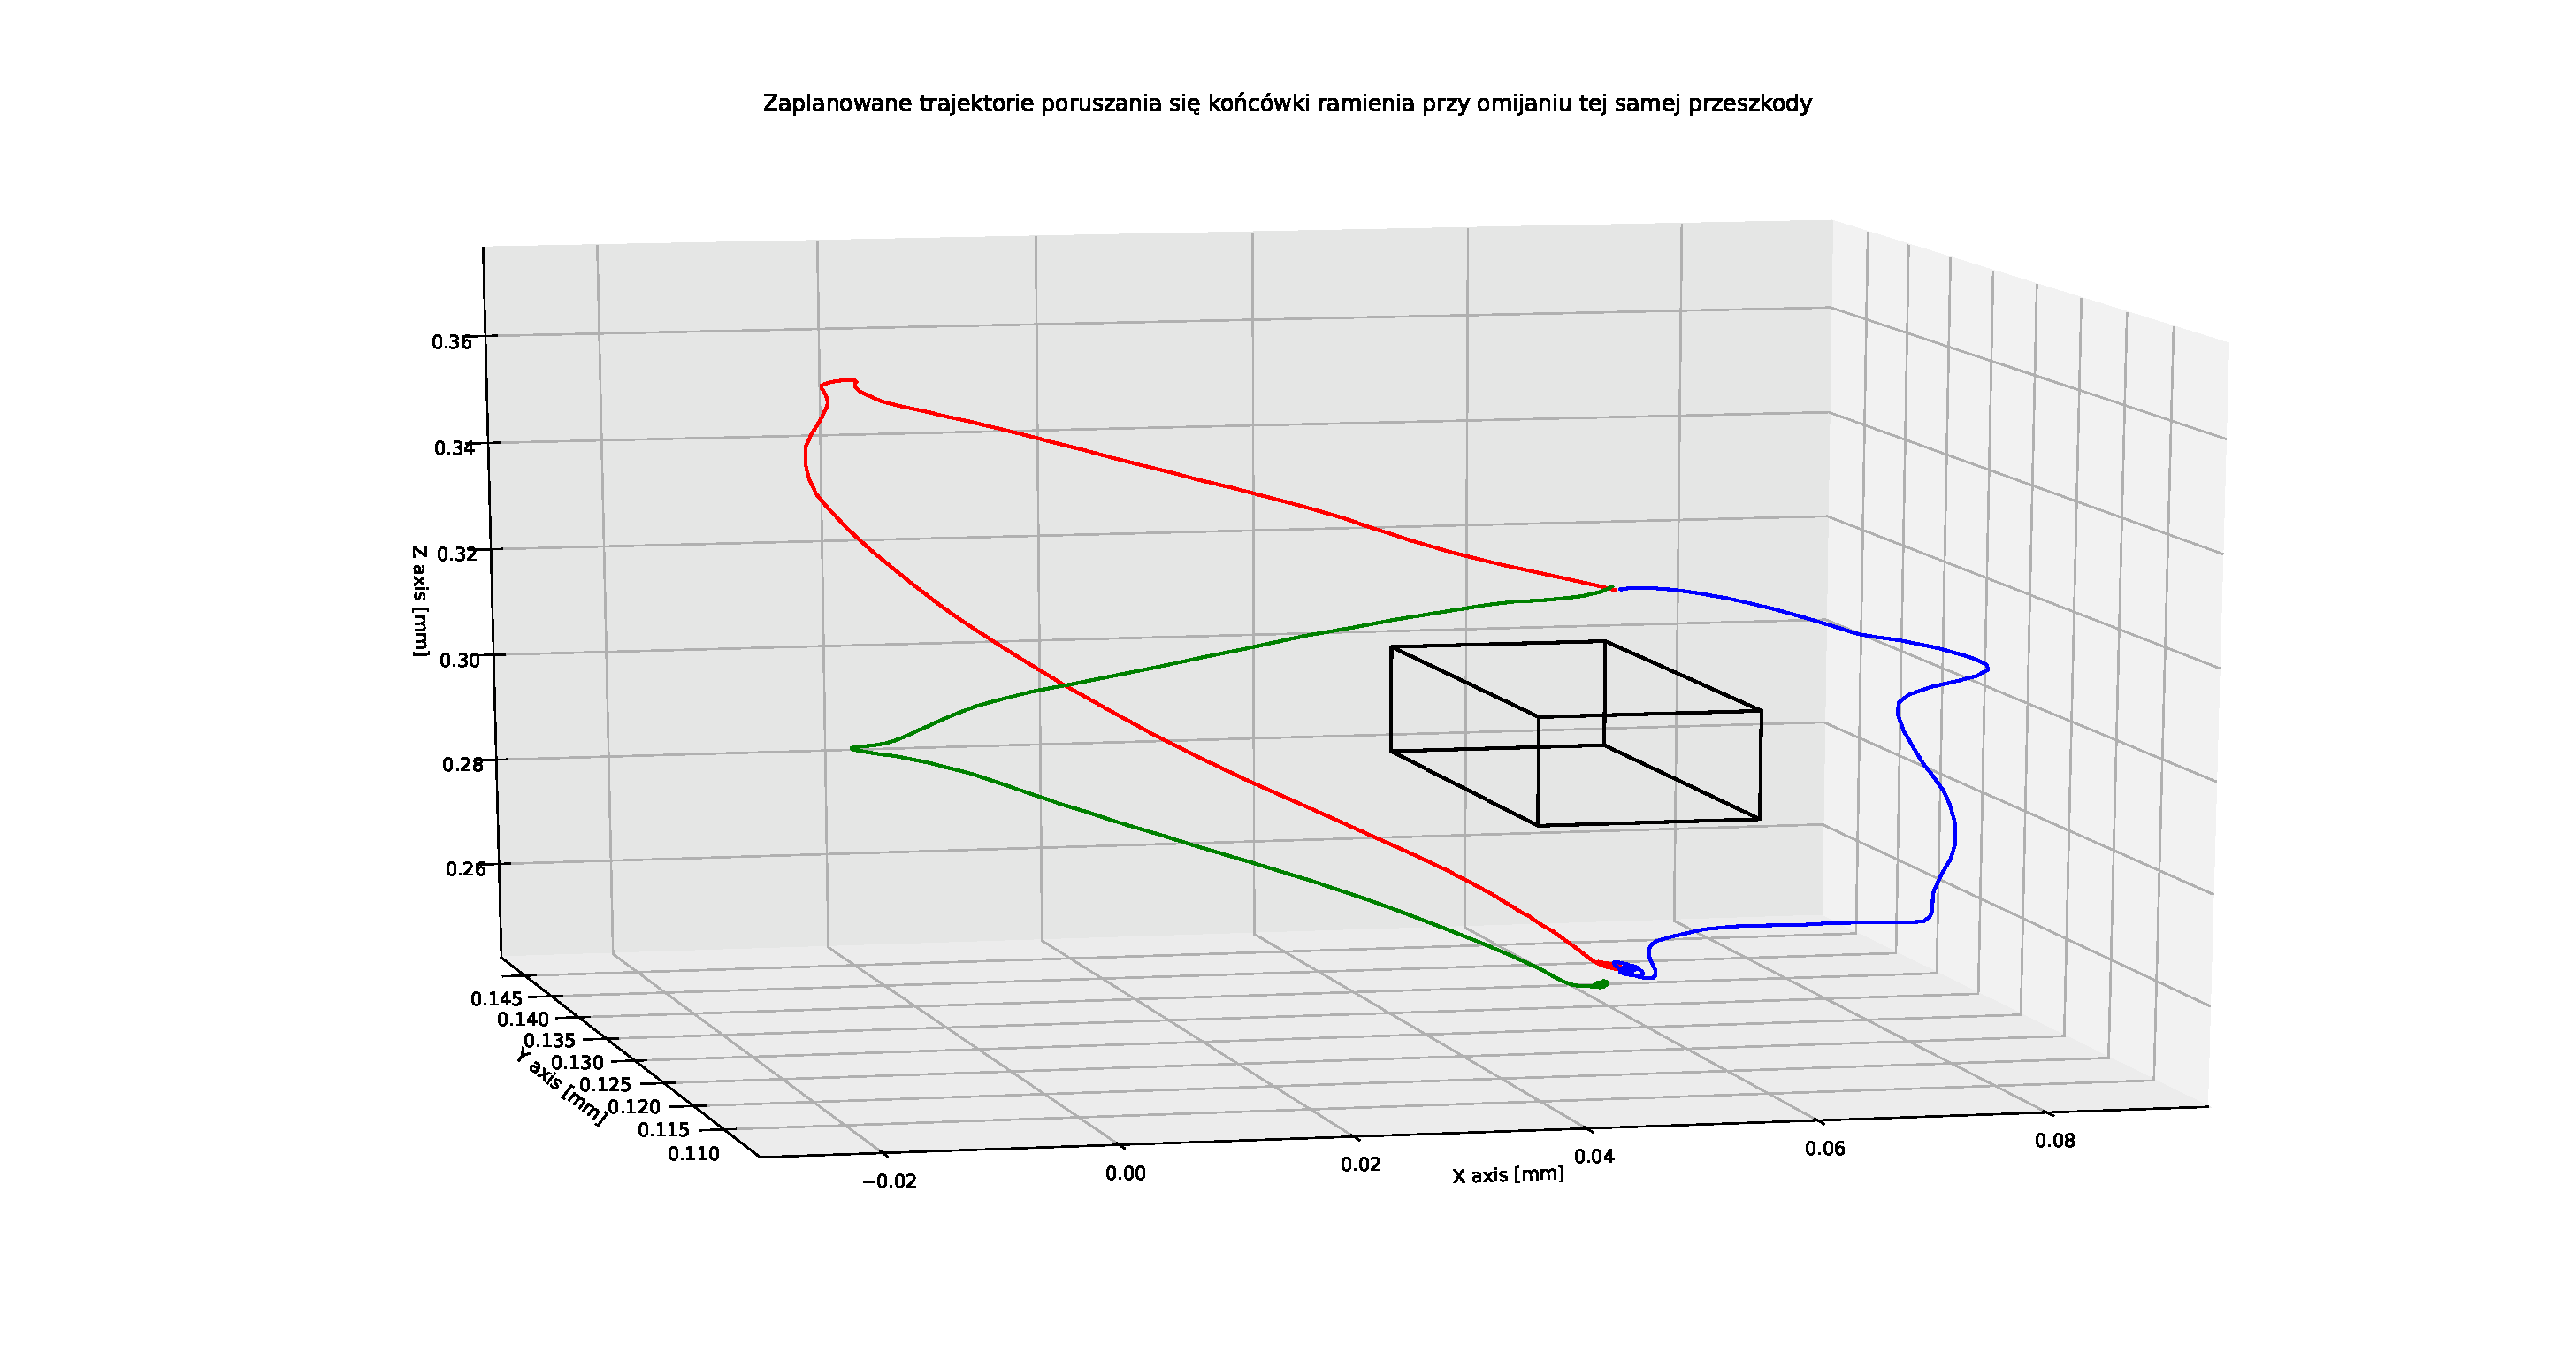
\includegraphics[width=1\linewidth]{{img/Figure_omitt.eps}}
	\caption{Zaplanowane trajektorie poruszania się końcówki ramienia przy omijaniu tej samej przeszkody. \cite{plot_file}}
	\label{fig:35}
\end{figure}

Podsumowując nieco zaprezentowane w tym podrozdziale eksperymenty, można powiedzieć, iż proces omijania przez manipulator nawet prostej przeszkody, nie jest zagadnieniem oczywistym. Plannery, które do tej pory uznawano za bardzo skuteczne (PTP, LIN, CHOMP) okazały się w ogóle nie realizować tego problemu. Niemniej pozytywną kwestią jest, iż istnieją algorytmy wchodzące w skład grupy OMPL, które bardzo dobrze radzą sobie z tym zagadnieniem, w konsekwencji czego, nadal MoveIt może służyć jako kontroler, także przy tego typu zastosowaniach.


\subsection{Trajektorie złożone}

Do tej pory testowano i porównywano ze sobą plannery jakie udostępniał MoveIt. Niezależnie od tego jakie trasy algorytmy te zaproponowały, były to trajektorie teoretyczne, po jakich miało się poruszać ramię robota. Niemniej w rzeczywistości robot nie podąża jednoznacznie za nimi, ze względu na ograniczenia konstrukcyjne i ogólnie fizykę. Toteż kolejna sekcja eksperymentów poświęcona została porównywaniu zachowań robota w środowisku symulacyjnym Gazebo oraz fizycznego urządzenia. 

Roboty przemysłowe są przystosowane do wykonywania często dwóch typów zadań. Pierwszym z nich jest klasyczne zadanie przenoszenia obiektów, tzw. zadanie $pick$ $and$ $place$.
Natomiast drugi typ zadań, jest związany ze sterowaniem robota w układzie kartezjańskim, tj. w sytuacji kiedy to końcówka robocza urządzenia utrzymuje np. stałą wysokość i orientację. Zadania takie są bardzo istotne np. w momencie spawania bądź nanoszenia kleju gdzie należy przesuwać ramię w jednej ustalonej płaszczyźnie, jednocześnie stale utrzymując zadaną odległość od obiektu.

Zaczynając od pierwszego ze wspomnianych zadań, postanowiono przygotować odpowiedni eksperyment. Jako, iż w oprogramowaniu Rviz nie jest możliwe wyznaczanie trajektorii złożonych, toteż napisano w tym celu węzeł ROS (język Python), który sekwencyjnie realizuje konieczną trasę. Robot nie został wyposażony w tor wizyjny, przez co trasę dobrano eksperymentalnie, docelowo powinien to realizować algorytm korzystający z zainstalowanych na urządzeniu kamer. \cite{PaP_file}

Jak wspominano w rozdziale poświęconym modelowi robota w Gazebo - \ref{sub:ModelGazebo}, do symulacji dodano niewielki obiekt, tak by urządzenie mogło go chwycić. Istotne było nadanie obiektowi należytych parametrów - takich jak masa, inercja oraz sprężystość. Bez nich robot nie był w stanie go przemieścić, gdyż albo był dla niego za ciężki, albo też nie dawał się złapać, ze względu na zbyt twardą powierzchnię. Parametry te jednocześnie nie powinny być także zbyt małe, gdyż wówczas manipulator nie był w stanie upuścić przedmiotu po przemieszczeniu. 

 \begin{figure}[H]
	\centering
	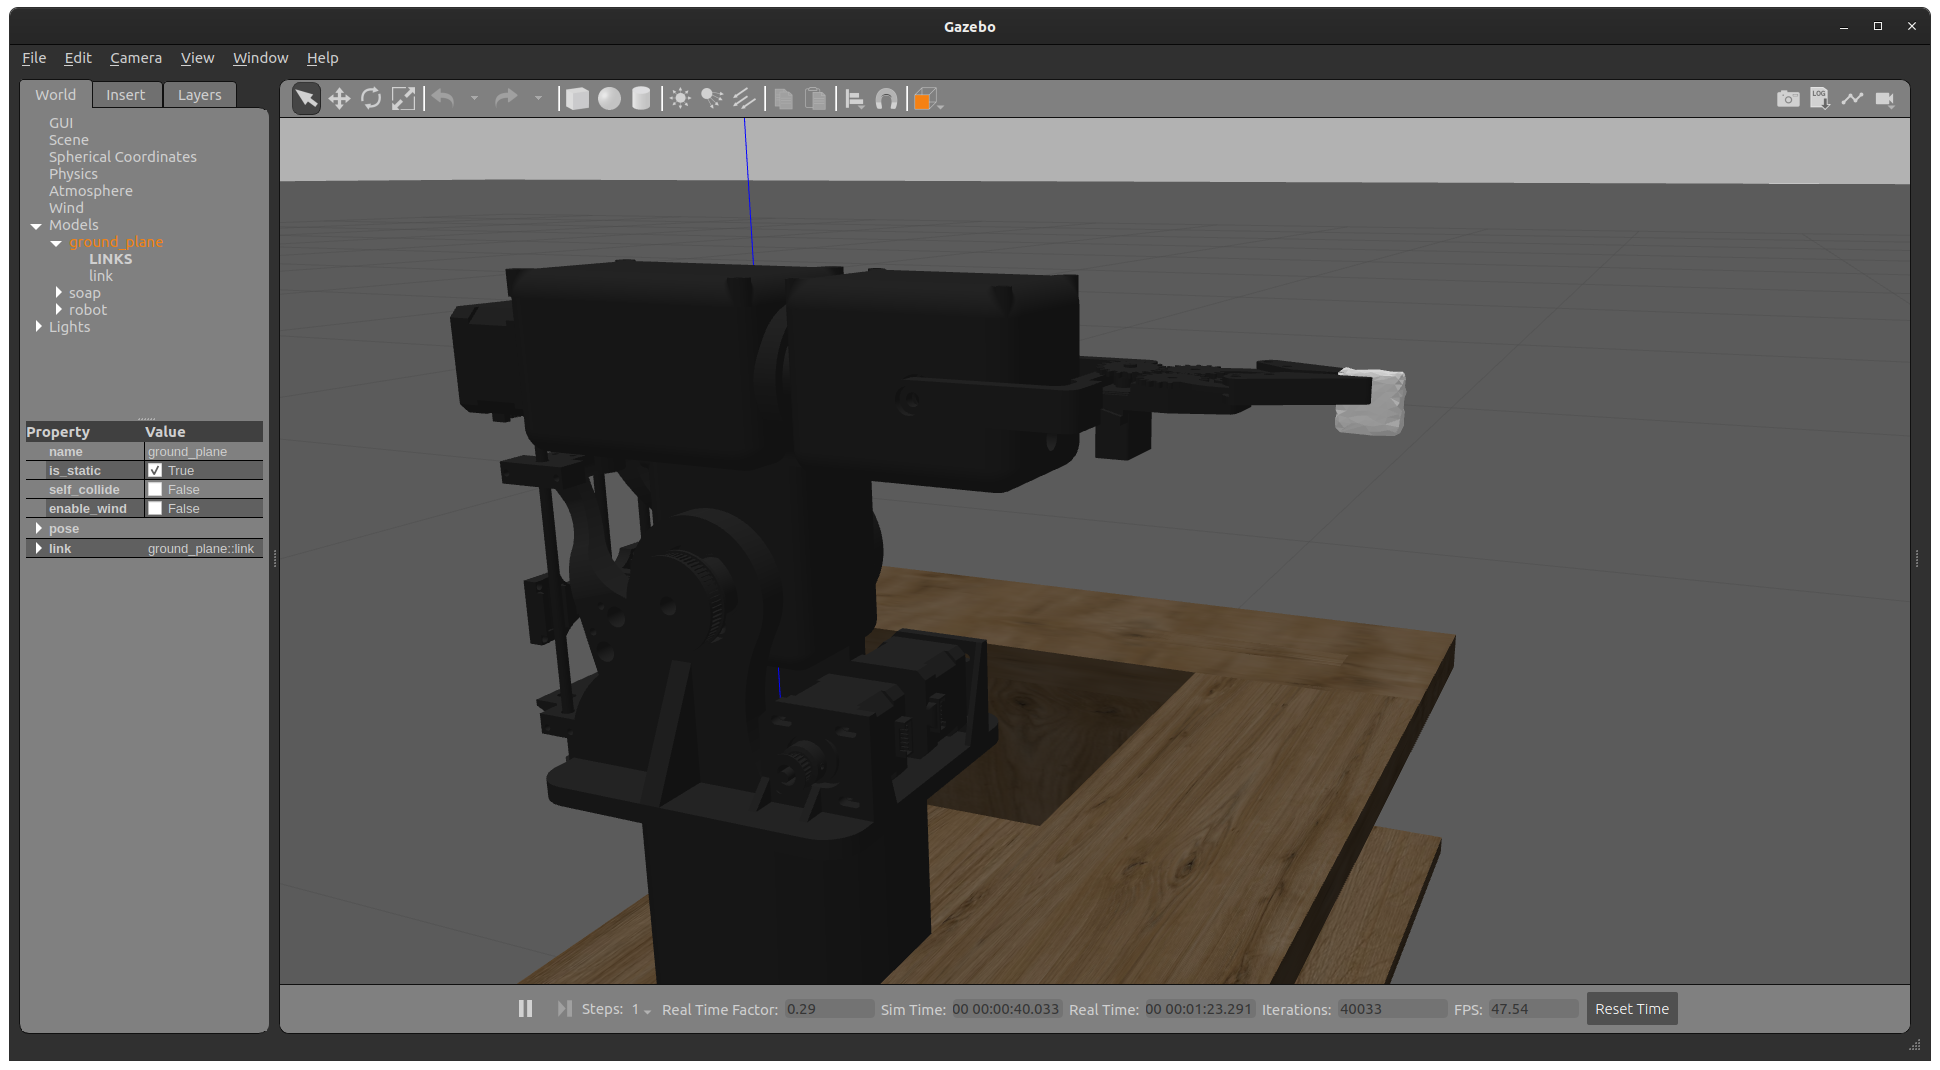
\includegraphics[width=1\linewidth]{{img/Bild_seife.png}}
	\caption{\centering Symulowany w Gazebo robot trzymający transportowany obiekt. \cite{own}, \cite{oak}}
	\label{fig:38}
\end{figure}

Uruchamiając sekwencję zbierano kolejne punkty w jakich znajdowało się urządzenie, tak by móc je później porównać ze sobą. Eksperyment przeprowadzono jednocześnie na symulacji oraz na faktycznym urządzeniu. W eksperymentach na fizycznym robocie wykorzystano pudełko zapałek, jako obiekt do transportu. W załącznikach do niniejszej pracy zamieszczono wideo, przedstawiające rzeczywistego robota realizującego opisywane zadanie. \cite{movie_file}

Uzyskanie punktów w przestrzeni kartezjańskiej dla rozwiązywanego zadania wymagało liczenia kinematyki prostej. Z wykorzystaniem ROS problem ten nie jest trudny do zrealizowania, gdyż udostępnia on funkcje, które na podstawie modelu robota (plik .urdf), przeliczają pozycje złączowe na punkty w przestrzeni.

Przeprowadzając eksperymenty zebrano pomiary, na podstawie których opracowano poniższy wykres - \ref{fig:36}

 \begin{figure}[H]
	\centering
	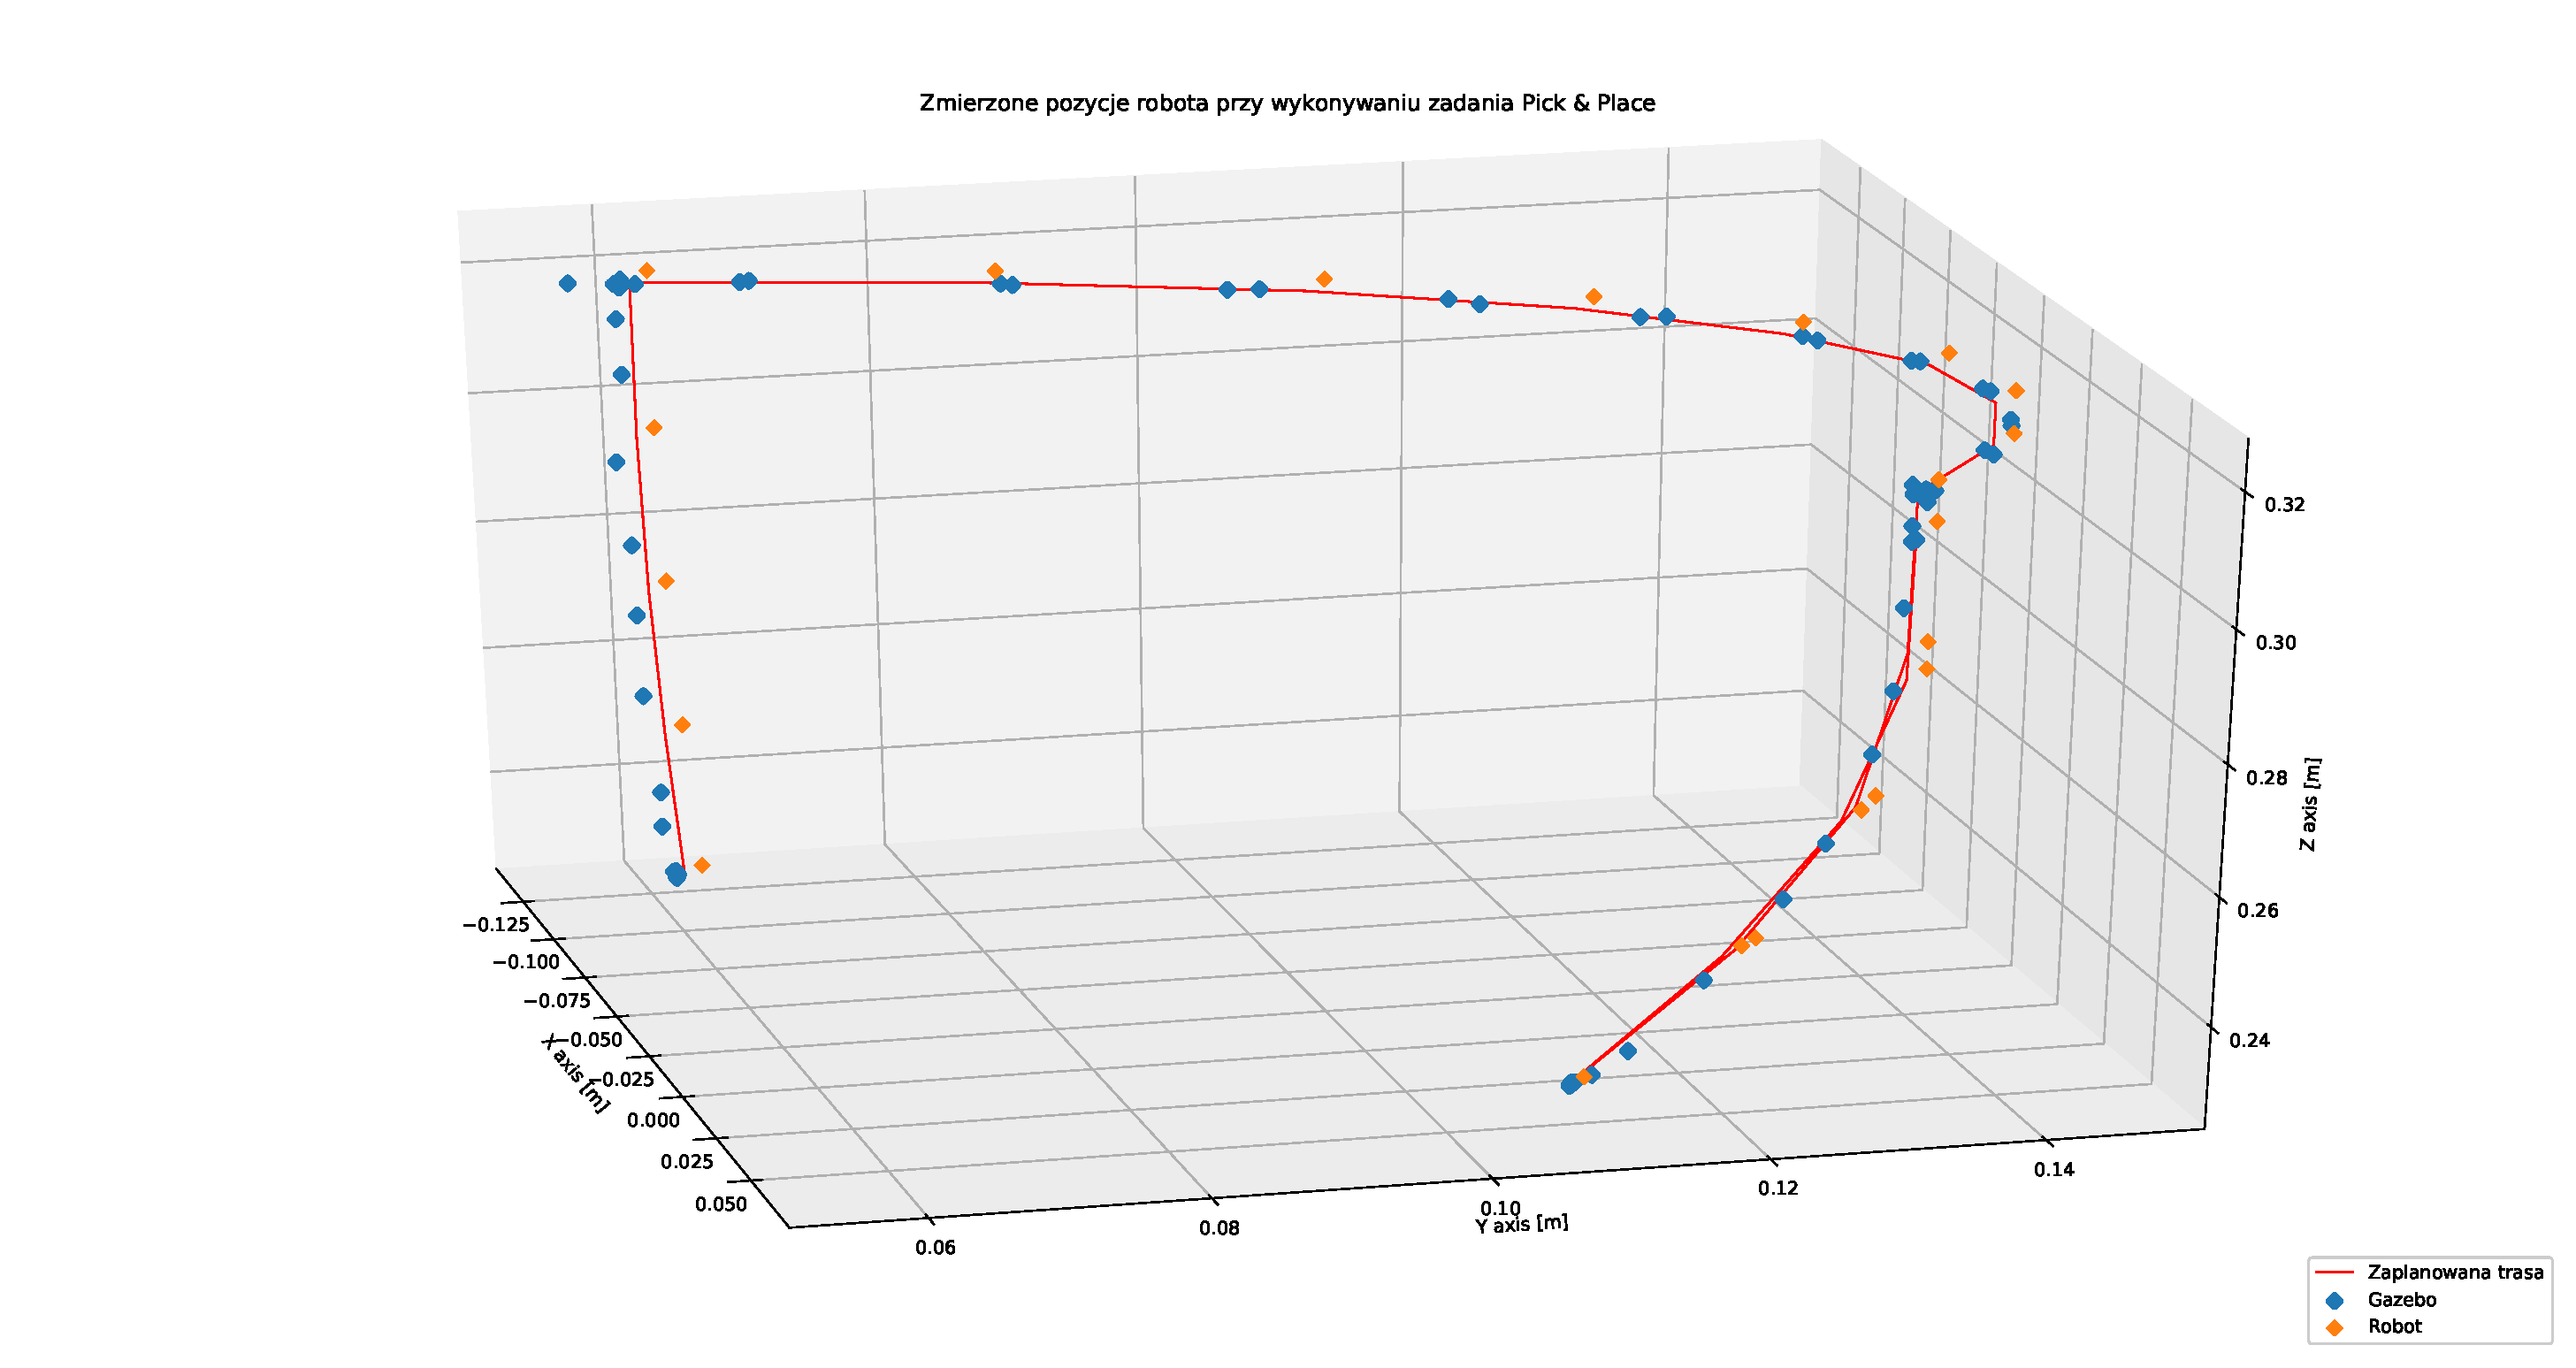
\includegraphics[width=1\linewidth]{{img/Figure_pap_com.eps}}
	\caption{Zmierzone pozycje robota przy wykonywaniu zadania Pick and Place. \cite{own}}
	\label{fig:36}
\end{figure}

Na podstawie zebranych punktów postanowiono policzyć różnicę między zaplanowaną trasą a faktycznymi punktami. Zatem kolejny raz posłużono się językiem Python. Napisano skrypt interpolujący punkty zaplanowanej trasy. W kolejnym kroku dla każdego pomiaru pochodzącego od Gazebo oraz z fizycznego robota policzono najkrótszy dystans do zinterplowanej krzywej. W ten sposób policzono minimalne odchylenie, maksymalne, a także wartość średnią.

% Please add the following required packages to your document preamble:
% \usepackage[table,xcdraw]{xcolor}
% If you use beamer only pass "xcolor=table" option, i.e. \documentclass[xcolor=table]{beamer}
\begin{table}[H]
\centering
\caption{Porównanie odchyleń zmierzonych punktów robota w czasie wykonywania zadania Pick \& Place}
\label{tab:8}
\begin{tabular}{|c|c|c|c|c|}
\hline
\rowcolor[HTML]{C0C0C0} 
Lp & Model  & \begin{tabular}[c]{@{}c@{}}Min.\\ odchyłka\\ {[}m{]}\end{tabular} & \cellcolor[HTML]{C0C0C0}\begin{tabular}[c]{@{}c@{}}Max.\\ odchyłka\\ {[}m{]}\end{tabular} & \begin{tabular}[c]{@{}c@{}}Śr.\\ odchyłka\\ {[}m{]}\end{tabular} \\ \hline
\rowcolor[HTML]{9AFF99} 
1. & Gazebo & 0.00010                                                           & 0.00396                                                                                   & 0.00066                                                          \\ \hline
\rowcolor[HTML]{FFCCC9} 
2. & Robot  & 0.00059                                                           & 0.00469                                                                                   & 0.00243                                                          \\ \hline
\end{tabular}
\end{table}


Teoretycznie model w Gazebo wypada w tym zestawieniu lepiej. Niemniej należy pamiętać, iż Gazebo realizuje ruch osi w oparciu o regulator PID i to w dużej mierze od jego nastaw zależy jak dobrze symulacją będzie podążała za zaplanowaną trasą. Natomiast faktyczny robot jest wyposażony w silniki krokowe. Zatem sterowanie nimi polega na podaniu ilości kroków jakie mają wykonać. Na tej podstawie wszystkie występujące zaokrąglenia do całkowitej liczby impulsów wprowadzają przekłamania. Kolejnym powodem dla którego faktyczny robot odznaczył się gorszą dokładnością jest występująca na złączą ramienia głównego nieliniowość. Wspominano już o tym w pracy inżynierskiej, iż sposób ukształtowania napędu ramienia głównego wprowadza pewne nieliniowości.


Drugi eksperyment dotyczył ruchu we współrzędnych kartezjańskich. Okazuje się, iż MoveIt również udostępnia tąże funkcjonalność. Podobnie jak to było wcześniej - nie można tego dokonać bezpośrednio z poziomu Rviza, toteż należało w tym celu napisać odpowiedni węzeł ROS. 

 \begin{figure}[H]
	\centering
	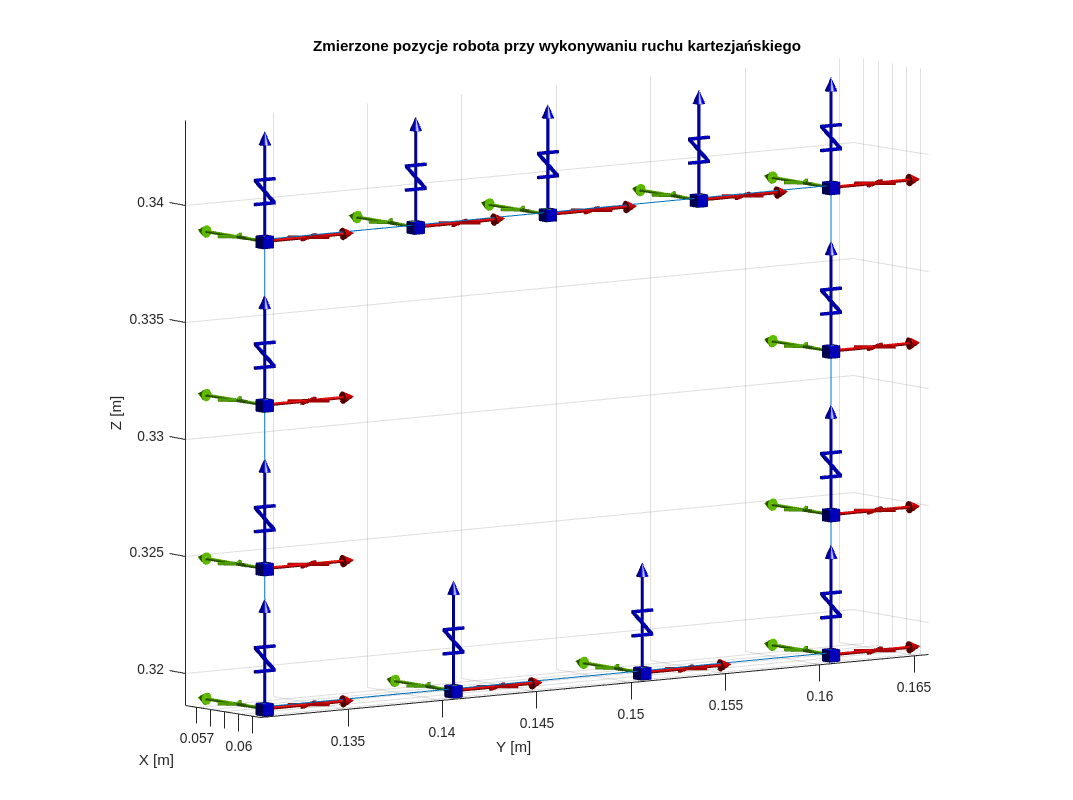
\includegraphics[width=1\linewidth]{{img/Figure_square.png}}
	\caption{Zaplanowana trajektoria przez planner dla realizacji przemieszczenia w układzie kartezjańskim. \cite{own}}
	\label{fig:37}
\end{figure}

Zaplanowano, iż ramię robota zakreśli czworokąt w płaszczyźnie pionowej. Napisano zatem węzeł - posłużywszy się językiem Python. Skrypt ten ładuje model robota z pliku URDF, następnie pobiera aktualny stan manipulatora, po czym nadsyła plannerowi kolejne punkty, które przyjęto na sztywno (wymiary czworokąta). \cite{Cart_file} 

Podobnie jak to miało miejsce wcześniej - tak i tym razem eksperymenty przeprowadzono zarówno dla symulacji w Gazebo jak i fizycznego robota. Powyżej zaprezentowano zaplanowaną przez planner trajektorię - rysunek \ref{fig:37}. Rysunek ten obrazuje również ideę przemieszczenia w układzie kartezjańskim. Jak widać pozycja złącza piątego (obrót chwytaka) zmienia się w taki sposób, iż stale utrzymywana jest konkretna płaszczyzna ruchu. Każdy punkt zaplanowany przez planner zaznaczono również niewielkim modelem układu współrzędnych, obrazującym orientację końcówki robota w przestrzeni. Można zauważyć iż jest ona stała. Takie zachowanie może być bardzo pożądane w niektórych zastosowaniach, takich jak wiercenie otworów, nakładanie warstwy kleju na szybę samochodu itp.  

Niemniej zaplanowana trasa jest trajektorią teoretyczną. Z tego też powodu rzeczywisty przebieg trajektorii robota zależy od jakości i precyzji jego wykonania. Dlatego poniżej zestawiono przestrzennie punkty pobrane w czasie symulowania ruchu manipulatora w programie Gazebo oraz z rzeczywistego urządzenia - \ref{fig:12}.  


\begin{figure}[H]
	\centering
	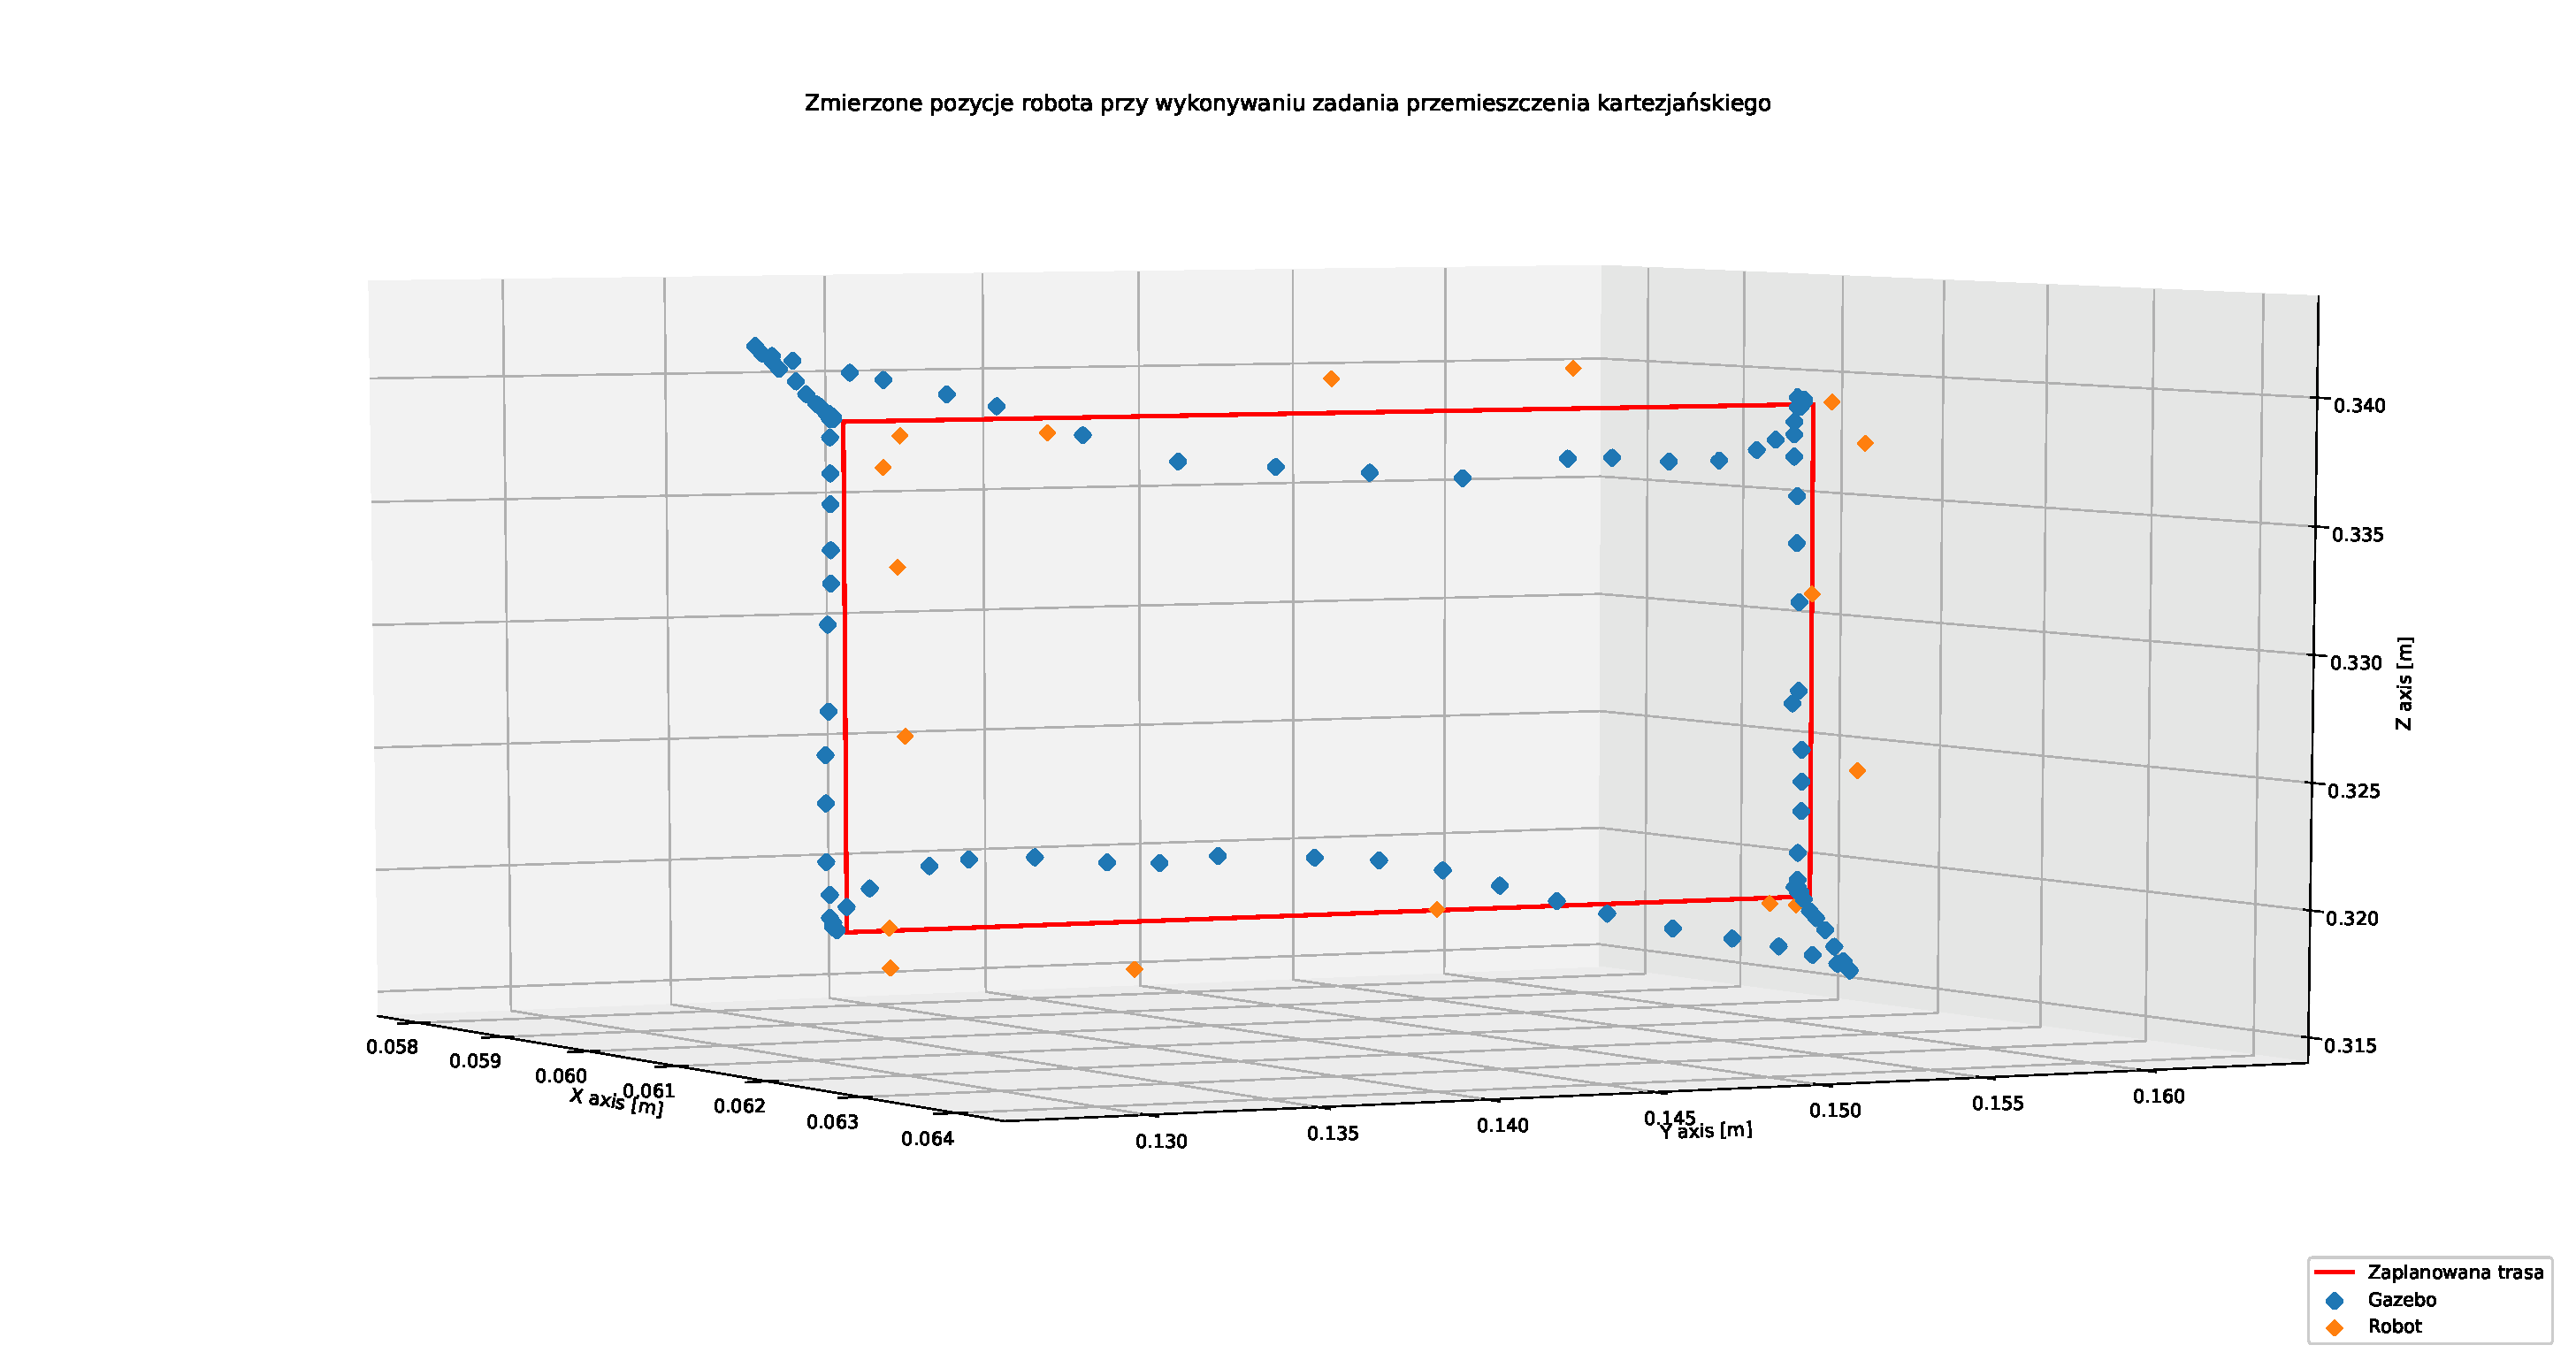
\includegraphics[width=1\linewidth]{{img/Figure_cartesian.eps}}
	\caption{Zmierzone pozycje robota przy wykonywaniu ruchu kartezjańskiego. \cite{own}}
	\label{fig:12}
\end{figure}

Jak widać w obu przypadkach trasa nie była idealna. Powodem, dla którego przebieg Gazebo znacznie odbiegał od pożądanego, były nastawy regulatora PID. W tym miejscu należy nadmienić, iż nastawy te należy dobrać zgodnie z masą oraz inercją złącz uwzględnioną w pliku URDF. Wartości te czerpano z fizycznych parametrów robota, niemniej po złym dobraniu nastawa regulatora (zbyt dużych bądź zbyt małych) w stosunku do opisanej fizyki robota, skutkuje przeróżnymi 'artefaktami' po uruchomieniu symulacji.

Jeżeli chodzi o wyniki rzeczywistego robota, to powody nieidealności jego przebiegu opisywano już wcześniej.

Dla końcowe podsumowania niniejszego eksperymentu, w poniższej tabeli zestawiono minimalne, maksymalne i średnie odchylenia od zaplanowanej trasy.


\begin{table}[H]
\centering
\caption{Porównanie odchyleń zmierzonych punktów robota w czasie wykonywania zadania przemieszczenia kartezjańskiego}
\label{tab:19}
\begin{tabular}{|c|c|c|c|c|}
\hline
\rowcolor[HTML]{C0C0C0} 
Lp & Model  & \begin{tabular}[c]{@{}c@{}}Min.\\ odchyłka\\ {[}m{]}\end{tabular} & \cellcolor[HTML]{C0C0C0}\begin{tabular}[c]{@{}c@{}}Max.\\ odchyłka\\ {[}m{]}\end{tabular} & \begin{tabular}[c]{@{}c@{}}Śr.\\ odchyłka\\ {[}m{]}\end{tabular} \\ \hline
\rowcolor[HTML]{FFCCC9} 
1. & Gazebo & 0.00051                                                           & 0.00866                                                                                   & 0.01181                                                          \\ \hline
\rowcolor[HTML]{9AFF99} 
2. & Robot  & 0.00054                                                           & 0.00139                                                                                   & 0.00210                                                          \\ \hline
\end{tabular}
\end{table}

W tym przypadku dokładniejszy okazał się fizyczny robot, niemniej jak wcześniej wspominano, jest to powiązane z nastawami regulatora.

Podsumowując przedstawione w niniejszym podrozdziale eksperymenty, można stwierdzić iż MoveIt nadaje się do generowania złożonych trajektorii i wykonywania przez manipulator konkretnych zadań. Wyznaczane trasy zależą jedynie od wyobraźni użytkownika oraz możliwości samego urządzenia. Jeżeli natomiast chodzi o otrzymane rezultaty związane z dokładnością odzwierciedlenia trasy, to nie były one idealne, jednak uwypukliły wrażliwe kwestie. Wiedza ta może zostać wykorzystana przy budowie kolejnych urządzeń bądź obsługi innych robotów.

\subsection{Sterowanie kartezjańskie i złączowe}

Zagadnieniem, które zdecydowano się również opisać jest różnica w ustalaniu nowej pozycji robota w programie Rviz, po modyfikacji parametru $position_only_ik$ pliku konfiguracyjnego $kinematics.yaml$. Parametr ten można ustawić na $True$ bądź $False$. Warunkuje on wyznaczanie nowych pozycji. W momencie gdy jest zanegowany wówczas użytkownik może modyfikować jedynie pozycje złącz. W momencie gdy został włączony wtedy wyznacza się pozycję robota w przestrzeni, do której ma zostać przesunięty, a nie samych osi. Wówczas też możliwe jest po prostu chwycenie myszką za interaktywny marker obecny na końcówce manipulatora i ustalenie nowej pozycji. W przypadku gdy włączone jest pozycjonowanie złącz opcja ta jest niemożliwa do wykonania. 



\begin{comment}


Jako że MoveIt wraz z ROSem udostępnia różne formy sterowania złączami w czasie realizacji trasy, toteż w tym podpunkcie postanowiono przetestować różnice w ich działaniu. \cite{Controllers}

Ze względu na uniwersalność oprogramowania ROS, pozwala on na sterowanie urządzeniami wykorzystującymi różne sposoby kontroli złącz. Oczywiście użytkownik może napisać swój dowolny sterownik, niemniej ROS domyślnie udostępnia trzy podstawowe.

Pierwszym z nich jest $Effort$ $Joint$ $Interface$ - dedykowany jest on robotom, których złącza sterowane są poprzez wartość siły, bądź momentu obrotowego.

Drugi - $Velocity$ $Joint$ $Interface$ - jak nazwa wskazuje jest przeznaczony do osi kontrolowanych przez określanie posiomu ich prędkości.

Ostatnim typem jest $Position$ $Joint$ $Interface$. W tym przypadku mowa o robotach, w których istotna jest jedynie pozycja danego członu.

Zatem postanowiono sprawdzić, jak różnią się sterowania oraz wiadomości wysyłane przez kontroler.


 \begin{figure}[H]
	\centering
	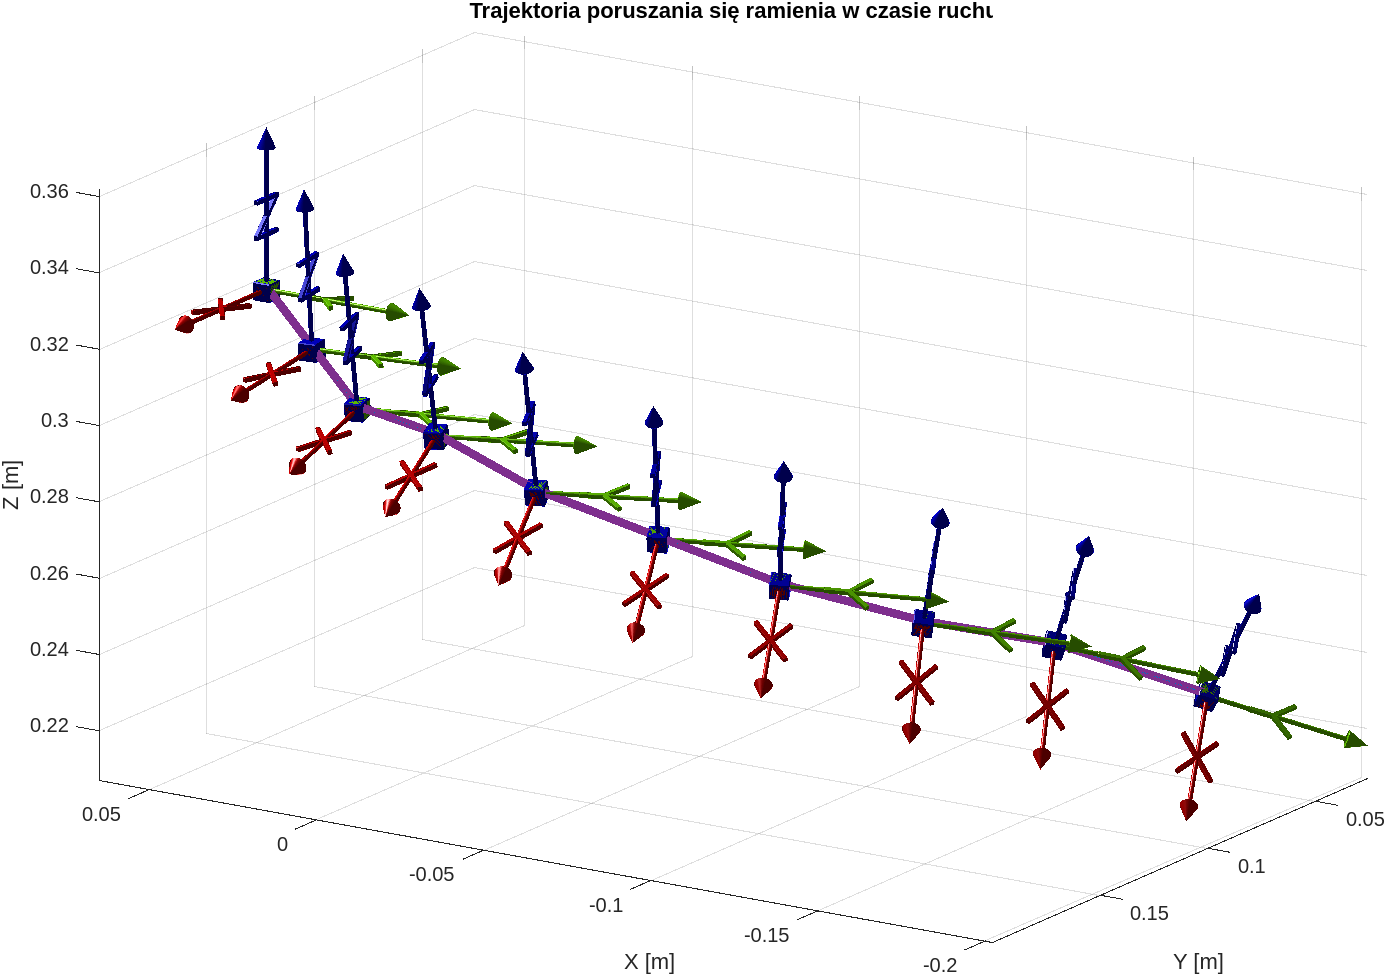
\includegraphics[width=0.9\linewidth]{{img/Figure_trajector.png}}
	\caption{Trajektoria poruszania się końcówki robota w czasie ruchu (DO WYMIANY, TYLKO TYP WYKRESU TEN SAM)}
	\label{fig:10}
\end{figure}


\subsection{Porównanie pluginów}

W czasie konfigurowania modelu robota w Setup Asisstant możliwy jest wybór pluginu, który będzie wykorzystywany na etapie rozwiązywania zadania kinematyki odwrotnej. Pierwszy z pluginów - $KDL Kinematics Plugin$ jest domyślny. Drugi - $LMA Kinematics Plugin$. Obie wtyczki posiadają podobne właściwości, gdyż w obu przypadkach opakowują one (ang. $wraps$) solvery kinematyki odwrotnej dostarczane przez paczkę $Orocos$ $KDL$. Oba pluginy zwracają uwagę na ograniczenia nałożone na poszczególne złącza, określone w plikach URDF. 

Postanowiono w związku z tym czy istnieje różnica w sposobie realizacji ruchu bądź planowania samej trasy między tymi dwoma pluginami. 

\cite{Plan_KDL_LMA}




\subsection{Ustawienia dodatkowe MoveIt}

Jako iż w programie Rviz, wtyczka MoveIt pozwala na określenie pewnych dodatkowych ustawień związanych z planowaniem oraz realizacją trasy, toteż postaniowo przetestować w jakim stopniu wpływają ustawienia te na proces wyznaczania trajektorii oraz jej bezpośrednią realizację.
Zatem użytkownik do dyspozycji posiada następujące ustawienia:
- $Use$ $Cartesian$ $Path$ - opcji tej należy użyć do wygenerowania liniwej trasy w przestrzeni kartezjańskiej. Opcja ta uniemożliwia planowania wokół przeszkód. Po jej zaznaczeniu uzyskano następujące rezultaty.


- $Colision$ $Avare$ $IK$ - 

- $Approx$ $IKSolutions$ - opcja ta dopuszcza przybliżone rozwiązania kinematyki odwrotnej, co jest przydatne w przypadku gdy punkt docelowy jest nieosiągalny. Po włączeniu tej opcji uzyskano:

- $External$ $ comm.$ - opcja ta udostępnia możliwość ustawiania punktów początkowych oraz końcowych jak również planowanie i wykonywanie trasy z poziomu zewnętrznych modułów. W tym celu konieczne jest po prostu wykorzystanie tematu /rviz/moveit.

Dwie kolejne opcje należą do grupy eksperymentalnych.
- $Replaning$ - opcja ta mogła zadziałać jedynie w przypadku uruchomienia komendy $Plan&Execute$, tj. gdy po planowaniu natychmiast następuje wykonanie trasy. W momencie gdy w czasie trwania ruchu zostanie wykryta kolizja, wtedy też trasa jest przeliczana na nowo.

- $Sensor$ $Positioning$ - była to ostatnia z opcji możliwa do użycia. Pozwala ona robotowi na zmianę pozycji swoich czujników, tak by możliwe było uniknięcie kolizji. (chyba to wywalę)


\subsection{Sposób ruchu złącz}

Głównym założeniem przyświecającym realizacji niniejszych eksperymentów było sprawdzenie, jak w czasie zmieniają się prędkości złącz przy realizacji ruchu. 
W tym celu zapisano ciągi sterowań wysyłane przez kontroler po czym najciekawsze przebiegi zestawiono zamieszczonych na wykresach. 



 \begin{figure}[H]
	\centering
	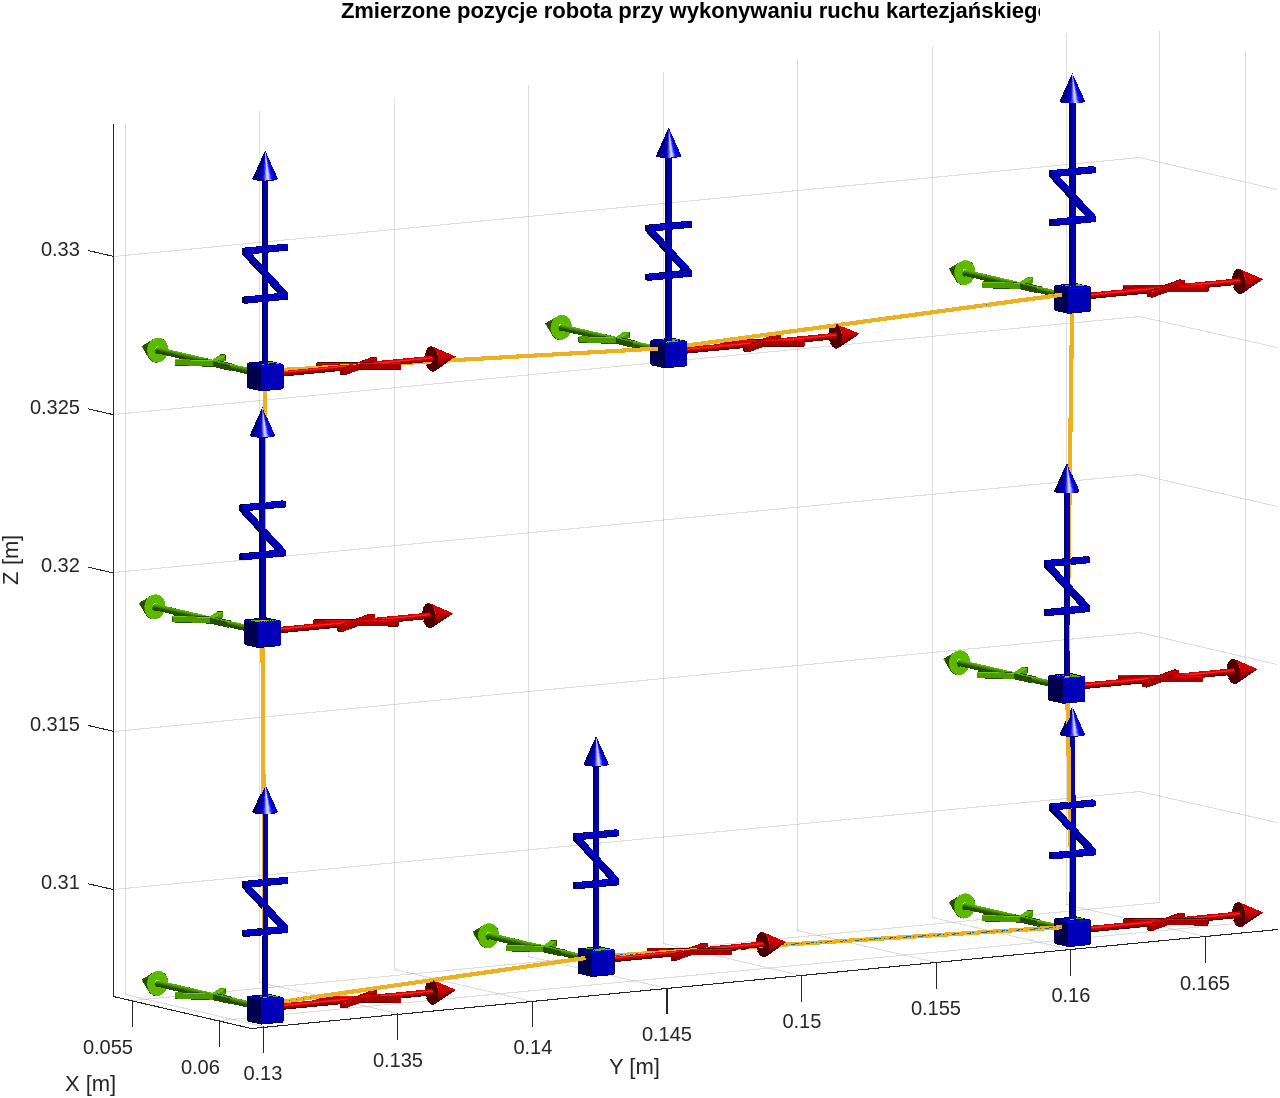
\includegraphics[width=0.8\linewidth]{{img/Figure_cartesian_2.png}}
	\caption{Zmierzone pozycje robota przy wykonywaniu ruchu kartezjańskiego (MOŻE DO WYMIANY)}
	\label{fig:13}
\end{figure}

 \begin{figure}[H]
	\centering
	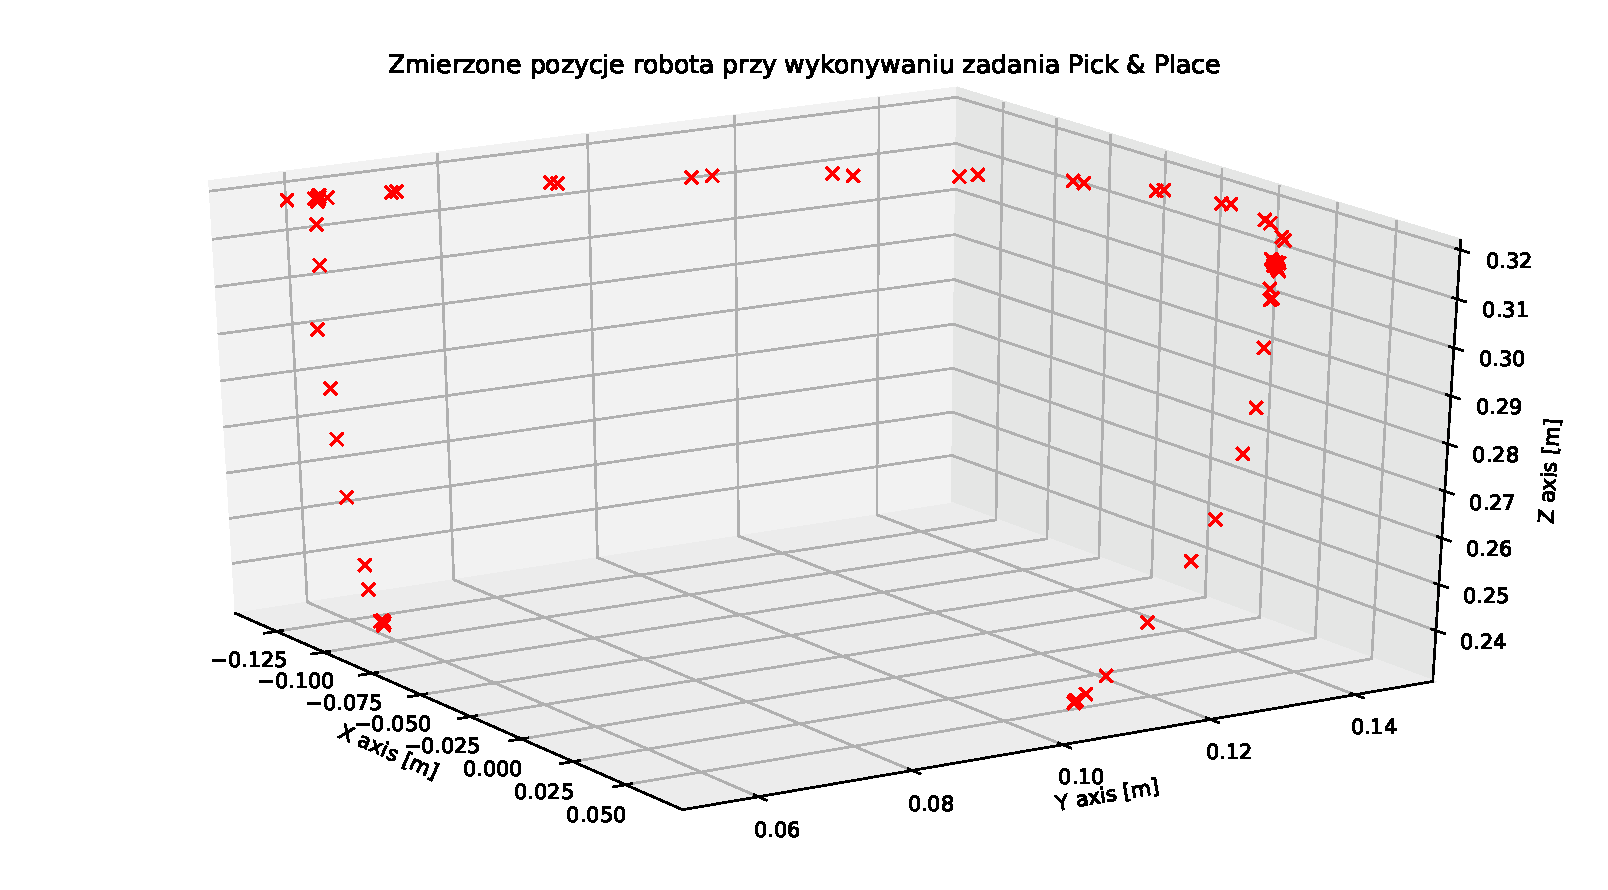
\includegraphics[width=0.8\linewidth]{{img/Figure_PaP.eps}}
	\caption{Zmierzone pozycje robota przy wykonywaniu ruchu kartezjańskiego (MOŻE DO WYMIANY)}
	\label{fig:14}
\end{figure}

\clearpage

\section{Testy dokładności (accuracy)}



\section{Testy powtarzalności (repeability)}

\section{Omijanie przeszkód}

Kolejnym z zaproponowanych testów było sprawdzenie czy dany planner jest w stanie omijać przeszkody a także w jaki sposób to czyni. W czasie różnych eksperymentów dało się zauważyć, że niektóre 
 z zaplanowanych tras są w znacznym stopniu nieoptymalne. Toteż postanowiono się przyjrzeń również tym aspektom. 

 W tym celu postanowiono napisać dodatkowy skrypt w języku python, którego glównym zadaniem było liczenie długości drogi kątowej jaką musiało pokonać poszczególne złącze, a także jak to się prezentowało sumarycznie. 


 % Please add the following required packages to your document preamble:
% \usepackage{multirow}
% \usepackage[table,xcdraw]{xcolor}
% If you use beamer only pass "xcolor=table" option, i.e. \documentclass[xcolor=table]{beamer}
\begin{table}[H]
\caption{Porównanie czasów planowania poszczególnych algorytmów}
\label{tab:4}
\begin{tabular}{|c|c|c|c|c|c|c|ll}
\cline{1-7}
\cellcolor[HTML]{C0C0C0}L.p. & \cellcolor[HTML]{C0C0C0}{\color[HTML]{000000} \begin{tabular}[c]{@{}c@{}}Grupa \\ plannerów\end{tabular}} & \cellcolor[HTML]{C0C0C0}Planner     & \cellcolor[HTML]{C0C0C0}\begin{tabular}[c]{@{}c@{}}Min. zapla. \\ trasa {[}rad{]}\end{tabular} & \cellcolor[HTML]{C0C0C0}\begin{tabular}[c]{@{}c@{}}Max. zapla.\\  trasa {[}rad{]}\end{tabular} & \cellcolor[HTML]{C0C0C0}\begin{tabular}[c]{@{}c@{}}Średnia\\  trasy {[}rad{]}\end{tabular} & \cellcolor[HTML]{C0C0C0}Uwagi &  &  \\ \cline{1-7}
\cellcolor[HTML]{EFEFEF}1.   & CHOMP                                                                                                     & \cellcolor[HTML]{EFEFEF}CHOMP       & \cellcolor[HTML]{EFEFEF}                                                                       & \cellcolor[HTML]{EFEFEF}                                                                       & \cellcolor[HTML]{EFEFEF}                                                                   & \cellcolor[HTML]{EFEFEF}      &  &  \\ \cline{1-7}
\cellcolor[HTML]{C0C0C0}2.   &                                                                                                           & \cellcolor[HTML]{C0C0C0}BFMT        & \cellcolor[HTML]{C0C0C0}                                                                       & \cellcolor[HTML]{C0C0C0}                                                                       & \cellcolor[HTML]{C0C0C0}                                                                   & \cellcolor[HTML]{C0C0C0}      &  &  \\ \cline{1-1} \cline{3-7}
\cellcolor[HTML]{EFEFEF}3.   &                                                                                                           & \cellcolor[HTML]{EFEFEF}BKPIECE     & \cellcolor[HTML]{EFEFEF}                                                                       & \cellcolor[HTML]{EFEFEF}                                                                       & \cellcolor[HTML]{EFEFEF}                                                                   & \cellcolor[HTML]{EFEFEF}      &  &  \\ \cline{1-1} \cline{3-7}
\cellcolor[HTML]{C0C0C0}4.   &                                                                                                           & \cellcolor[HTML]{C0C0C0}BiEST       & \cellcolor[HTML]{C0C0C0}                                                                       & \cellcolor[HTML]{C0C0C0}                                                                       & \cellcolor[HTML]{C0C0C0}                                                                   & \cellcolor[HTML]{C0C0C0}      &  &  \\ \cline{1-1} \cline{3-7}
\cellcolor[HTML]{EFEFEF}5.   &                                                                                                           & \cellcolor[HTML]{EFEFEF}BiTRRT      & \cellcolor[HTML]{EFEFEF}                                                                       & \cellcolor[HTML]{EFEFEF}                                                                       & \cellcolor[HTML]{EFEFEF}                                                                   & \cellcolor[HTML]{EFEFEF}      &  &  \\ \cline{1-1} \cline{3-7}
\cellcolor[HTML]{C0C0C0}6.   &                                                                                                           & \cellcolor[HTML]{C0C0C0}EST         & \cellcolor[HTML]{C0C0C0}                                                                       & \cellcolor[HTML]{C0C0C0}                                                                       & \cellcolor[HTML]{C0C0C0}                                                                   & \cellcolor[HTML]{C0C0C0}      &  &  \\ \cline{1-1} \cline{3-7}
\cellcolor[HTML]{EFEFEF}7.   &                                                                                                           & \cellcolor[HTML]{EFEFEF}FMT         & \cellcolor[HTML]{EFEFEF}                                                                       & \cellcolor[HTML]{EFEFEF}                                                                       & \cellcolor[HTML]{EFEFEF}                                                                   & \cellcolor[HTML]{EFEFEF}      &  &  \\ \cline{1-1} \cline{3-7}
\cellcolor[HTML]{C0C0C0}8.   &                                                                                                           & \cellcolor[HTML]{C0C0C0}KPIECE      & \cellcolor[HTML]{C0C0C0}                                                                       & \cellcolor[HTML]{C0C0C0}                                                                       & \cellcolor[HTML]{C0C0C0}                                                                   & \cellcolor[HTML]{C0C0C0}      &  &  \\ \cline{1-1} \cline{3-7}
\cellcolor[HTML]{EFEFEF}9.   &                                                                                                           & \cellcolor[HTML]{EFEFEF}LBKPIECE    & \cellcolor[HTML]{EFEFEF}                                                                       & \cellcolor[HTML]{EFEFEF}                                                                       & \cellcolor[HTML]{EFEFEF}                                                                   & \cellcolor[HTML]{EFEFEF}      &  &  \\ \cline{1-1} \cline{3-7}
\cellcolor[HTML]{C0C0C0}10.  &                                                                                                           & \cellcolor[HTML]{C0C0C0}LBTRRT      & \cellcolor[HTML]{C0C0C0}                                                                       & \cellcolor[HTML]{C0C0C0}                                                                       & \cellcolor[HTML]{C0C0C0}                                                                   & \cellcolor[HTML]{C0C0C0}      &  &  \\ \cline{1-1} \cline{3-7}
\cellcolor[HTML]{EFEFEF}11.  &                                                                                                           & \cellcolor[HTML]{EFEFEF}LazyPRM     & \cellcolor[HTML]{EFEFEF}                                                                       & \cellcolor[HTML]{EFEFEF}                                                                       & \cellcolor[HTML]{EFEFEF}                                                                   & \cellcolor[HTML]{EFEFEF}      &  &  \\ \cline{1-1} \cline{3-7}
\cellcolor[HTML]{C0C0C0}12.  &                                                                                                           & \cellcolor[HTML]{C0C0C0}LazyPRMstar & \cellcolor[HTML]{C0C0C0}                                                                       & \cellcolor[HTML]{C0C0C0}                                                                       & \cellcolor[HTML]{C0C0C0}                                                                   & \cellcolor[HTML]{C0C0C0}      &  &  \\ \cline{1-1} \cline{3-7}
\cellcolor[HTML]{EFEFEF}13.  &                                                                                                           & \cellcolor[HTML]{EFEFEF}PDST        & \cellcolor[HTML]{EFEFEF}                                                                       & \cellcolor[HTML]{EFEFEF}                                                                       & \cellcolor[HTML]{EFEFEF}                                                                   & \cellcolor[HTML]{EFEFEF}      &  &  \\ \cline{1-1} \cline{3-7}
\cellcolor[HTML]{C0C0C0}14.  &                                                                                                           & \cellcolor[HTML]{C0C0C0}PRM         & \cellcolor[HTML]{C0C0C0}                                                                       & \cellcolor[HTML]{C0C0C0}                                                                       & \cellcolor[HTML]{C0C0C0}                                                                   & \cellcolor[HTML]{C0C0C0}      &  &  \\ \cline{1-1} \cline{3-7}
\cellcolor[HTML]{EFEFEF}15.  &                                                                                                           & \cellcolor[HTML]{EFEFEF}PRMstar     & \cellcolor[HTML]{EFEFEF}                                                                       & \cellcolor[HTML]{EFEFEF}                                                                       & \cellcolor[HTML]{EFEFEF}                                                                   & \cellcolor[HTML]{EFEFEF}      &  &  \\ \cline{1-1} \cline{3-7}
\cellcolor[HTML]{C0C0C0}16.  &                                                                                                           & \cellcolor[HTML]{C0C0C0}ProjEST     & \cellcolor[HTML]{C0C0C0}                                                                       & \cellcolor[HTML]{C0C0C0}                                                                       & \cellcolor[HTML]{C0C0C0}                                                                   & \cellcolor[HTML]{C0C0C0}      &  &  \\ \cline{1-1} \cline{3-7}
\cellcolor[HTML]{EFEFEF}11.  &                                                                                                           & \cellcolor[HTML]{EFEFEF}RRTConnect  & \cellcolor[HTML]{EFEFEF}                                                                       & \cellcolor[HTML]{EFEFEF}                                                                       & \cellcolor[HTML]{EFEFEF}                                                                   & \cellcolor[HTML]{EFEFEF}      &  &  \\ \cline{1-1} \cline{3-7}
\cellcolor[HTML]{C0C0C0}12.  &                                                                                                           & \cellcolor[HTML]{C0C0C0}RRT         & \cellcolor[HTML]{C0C0C0}                                                                       & \cellcolor[HTML]{C0C0C0}                                                                       & \cellcolor[HTML]{C0C0C0}                                                                   & \cellcolor[HTML]{C0C0C0}      &  &  \\ \cline{1-1} \cline{3-7}
\cellcolor[HTML]{EFEFEF}13.  &                                                                                                           & \cellcolor[HTML]{EFEFEF}RRTstar     & \cellcolor[HTML]{EFEFEF}                                                                       & \cellcolor[HTML]{EFEFEF}                                                                       & \cellcolor[HTML]{EFEFEF}                                                                   & \cellcolor[HTML]{EFEFEF}      &  &  \\ \cline{1-1} \cline{3-7}
\cellcolor[HTML]{C0C0C0}14.  &                                                                                                           & \cellcolor[HTML]{C0C0C0}SBL         & \cellcolor[HTML]{C0C0C0}                                                                       & \cellcolor[HTML]{C0C0C0}                                                                       & \cellcolor[HTML]{C0C0C0}                                                                   & \cellcolor[HTML]{C0C0C0}      &  &  \\ \cline{1-1} \cline{3-7}
\cellcolor[HTML]{EFEFEF}15.  &                                                                                                           & \cellcolor[HTML]{EFEFEF}SPARS       & \cellcolor[HTML]{EFEFEF}                                                                       & \cellcolor[HTML]{EFEFEF}                                                                       & \cellcolor[HTML]{EFEFEF}                                                                   & \cellcolor[HTML]{EFEFEF}      &  &  \\ \cline{1-1} \cline{3-7}
\cellcolor[HTML]{C0C0C0}16.  &                                                                                                           & \cellcolor[HTML]{C0C0C0}SPARStwo    & \cellcolor[HTML]{C0C0C0}                                                                       & \cellcolor[HTML]{C0C0C0}                                                                       & \cellcolor[HTML]{C0C0C0}                                                                   & \cellcolor[HTML]{C0C0C0}      &  &  \\ \cline{1-1} \cline{3-7}
\cellcolor[HTML]{EFEFEF}17.  &                                                                                                           & \cellcolor[HTML]{EFEFEF}STRIDE      & \cellcolor[HTML]{EFEFEF}                                                                       & \cellcolor[HTML]{EFEFEF}                                                                       & \cellcolor[HTML]{EFEFEF}                                                                   & \cellcolor[HTML]{EFEFEF}      &  &  \\ \cline{1-1} \cline{3-7}
\cellcolor[HTML]{C0C0C0}18.  & \multirow{-23}{*}{OMPL}                                                                                   & \cellcolor[HTML]{C0C0C0}TRRT        & \cellcolor[HTML]{C0C0C0}                                                                       & \cellcolor[HTML]{C0C0C0}                                                                       & \cellcolor[HTML]{C0C0C0}                                                                   & \cellcolor[HTML]{C0C0C0}      &  &  \\ \cline{1-7}
\cellcolor[HTML]{EFEFEF}19.  &                                                                                                           & \cellcolor[HTML]{EFEFEF}PTP         & \cellcolor[HTML]{EFEFEF}                                                                       & \cellcolor[HTML]{EFEFEF}                                                                       & \cellcolor[HTML]{EFEFEF}                                                                   & \cellcolor[HTML]{EFEFEF}      &  &  \\ \cline{1-1} \cline{3-7}
\cellcolor[HTML]{C0C0C0}20.  & \multirow{-2}{*}{\begin{tabular}[c]{@{}c@{}}Pilz Industrial \\ \\ Motion Planner\end{tabular}}            & \cellcolor[HTML]{C0C0C0}LIN         & \cellcolor[HTML]{C0C0C0}                                                                       & \cellcolor[HTML]{C0C0C0}                                                                       & \cellcolor[HTML]{C0C0C0}                                                                   & \cellcolor[HTML]{C0C0C0}      &  &  \\ \cline{1-7}
\end{tabular}
\end{table}

\end{comment}

\section{Podsumowanie rozdziału}

Podsumowując przeprowadzone w niniejszym rozdziale liczne testy, można stwierdzić iż MoveIt udostępnia użytkownikom spory zakres funkcjonalności. Liczba możliwych do użycia plannerów, opcji, sposobów poruszania, jest znaczna. Rozwiązanie problemu kinematyki odwrotnej nie jest zadaniem prostym, jednak MoveIt posiada solvery takie wbudowane w siebie. Pozwala to na znaczące skrócenie czasu rozwoju projektu nowego robota. Musząc samemu stworzyć planner trajektorii, prawdopodobnie zrealizowano by to mało optymalnie. MoveIt nie tylko udostępnia takie rozwiązania gotowe, co również pozwala na wybieranie między nimi. W ten sposób można skupić się jedynie na kwestii obierania sygnałów sterujących od MoveIta i ich odpowiednie przetwarzanie bezpośrednio na wymagane ruchy silników.

Na pewno korzystanie z ROSa wprowadza pewne ograniczenia, narzuca pewne standardy, niemniej możliwości konfiguracyjne oraz edytorskie są na tyle duże, iż praktycznie każdą funkcjonalność, która w pewnym stopniu użytkownikowi nie odpowiada można zmodfikować badź po prostu napisać własną.


	\chapter{Podsumowanie i wnioski końcowe}

Zrealizowany projekt pozwala wysnuć wnioski, iż oprogramowanie ROS wraz z dodatkiem MoveIt, mimo pewnych ograniczeń w dobrym stopniu nadaje się do sterowania robotem. W czasie przeprowadzanych eksperymentów możliwe było zaobserwowanie, iż w pewnym momencie dochodziło się do swoistych fizycznych ograniczeń związanych z konstrukcją samego robota (powstały jako wydruk 3D), przez co niemożliwe było uzyskiwanie chociażby dokładniejszych sposobów pozycjonowania. Niemniej projekt miał na celu bardziej przetestować funkcjonalność, możliwości kontroli urządzenia, co też udało się w pełni. 

Jeżeli chodzi o samo oprogramowanie ROS to istotnie znacząco ułatwia ono i przede wszystkim standaryzuje kwestie związane ze sterowaniem budowanymi robotami. Przy czym niezbędne jest poświęcenie sporej ilości czasu na jego zainstalowanie, uruchomienie i skonfigurowanie. Dla wielu potencjalnych użytkowników może to stanowić barierę zniechęcającą do zapoznawania się z tym środowiskiem, ze względu na ograniczoną społeczność innych programistów oraz nierzadko niepełną dokumentację, przez co wielokrotnie rozwiązania wielu napotkanych problemów należy poszukiwać samodzielnie, co nierzadko zajmuje całe tygodnie. Podobnie było przy realizacji tego projektu, gdzie trudności stanowiło już zainstalowanie samego ROSa, ze względu na potrzebę rozwiązania konfliktów przy buildowaniu plików. Tak zatem w początkowej fazie użytkowania oprogrmowania ROS większość czasu poświęca się na rozwiązywaniu występujących błędów, aniżeli samym pisaniu kodu.

W czasie realizacji projektu wyszły również na jaw kwestie związane z fizycznymi ograniczeniami posiadanego robota. Jako, iż został on w całości wydrukowany a części jakie użyto do jego budowy należą raczej do rozwiązań nieprzemysłowych, toteż cała konstrukcja wyróżniała się dosyć sporą zawodnością. Przede wszystkim przewody do prototypowania, którymi łączono sporo elementów elektroniczynych, pinów mikrokontrolera z czujnikami, sterownikami silników krokowych nierzadko nie spełniały swoich funkcji. Przez przypadek wypadały, nie łączyły jak powinny. W pewnym momencie prototyp robota był na tyle złożony, iż chcą ewentualnie w przyszłości dalej rozwijać konstrukcję, konieczne by było wymienić zawodne elementy - takie jak chociażby wspomniane przewody do prototypowania na solidniejsze połączenia.

Podobnie kwestia miała się z faktem luzów robota obecnych na poszczególnych złączach. Fakt, iż robot został wydrukowany, również niektóre jego przekładnie napędowe powstały w ten sposób, powoduje iż poszczególne osie charakteryzują się sporymi luzami na poziomie jednego bądz nawet dwóch stopni. Przez to trudno mówić o wyjątkowej dokładności urządzenia. O ile w przypadku rozpatrywanego robota nie stanowiło to większe problemu, gdyż powstała platforma miała formę eksperymentalną, edukacyjną, o tyle dla bardziej profesjonalnych zastosowań niezbędne byłyby znacznie precyzyjniejsze rozwiązania. Niestety też znacznie droższe. 

Należy również wspomnieć o wpływie grawitacji na ruch złącz na które siła ta działa. Dało się zauważyć, iż ramię drugie robota, w przypadku którego wpływ grawitacji był największy poruszało się z różną prędkością w zależności od kierunku ruchu. Tym samym, przy opuszczaniu ramię przekraczało zadaną pozycję. W przeciwnym kierunku, przy podnoszeniu ten problem nie występował.

Nie da się także nie zauważyć ograniczeń konstrukcyjnych jakie posiadała konstrukcja robota wykorzystanego w projekcie. Warto tutaj wymienić takie szczegóły jak niewielki zakres ruchu poszczególnych ramion, a także niewielką liczbę stopni swobody. Wydaje się iż szósta bądź nawet siódma oś pozwalałaby na zwielokrotnienie możliwości konstrukcji.

Na temat samego chwytaka również nasuwają się pewne wnioski. Z prowadzonych eksperymentów wynikało, iż człon chwytający powinien posiadać pewną formę sprzężenia zwrotnego związanego z siłą chwytu. Problematyczne też okazało się sterowanie chwytakiem poprzez współczynnik wypełnienia. Niestety ale przewody zasilające, biegnące bez ekranowania w pobliżu silników krokowych były narażone na zakłócenia. 

Dodatkowo posiadany robot posiadał zbyt mało stopni swobody by móc realizować zadanie nullspace exploration - czyli sytuacji kiedy to końcówka, kiść robota nie pozostaje w tym samej pozycji natomiast całe ramię wykonuje swoisty ruch okrężny. \cite{latex_code}
 
	% itd.
	% \appendix
	% \include{dodatekA}
	% \include{dodatekB}
	% itd.
	
	% \printbibliography
        \printbibheading[heading=bibintoc]
        \printbibliography[heading=subbibintoc, keyword=bibl,title=Źródła internetowe i książki]
         \printbibliography[heading=subbibintoc,keyword=image, title=Źródła zdjęć i rysunków ]
        \printbibliography[heading=subbibintoc,keyword=code, title=Wykorzystane kody źródłowe i modele]   
        \printbibliography[heading=subbibintoc,keyword=atta, title=Załączniki ]  

        
        % \printbibheading[heading=subbibintoc,title=Źródła zdjęć i rysunków]


\end{document}
